%!TEX root = main.tex
%%%%%%%%%%%%%%%%%%%%%%%%%%%%%%%%%%%%%%%%%%%%%%%%%%%%%%%%%%%%%%%%%%%%%%%%%%%%%%%%%%%%%%%%%%%%%%%%%%%%%%
%
%   Filename    : chapter_4.tex 
%
%   Description : This file will contain your System Framework. About the system, pipline, use cases, anything that has to do with constructions and parts of the actual software/system. An overall look on the background of the system. Not sure which approach kung top down or reverse ba or some other way. Sorry fam.
%                 
%%%%%%%%%%%%%%%%%%%%%%%%%%%%%%%%%%%%%%%%%%%%%%%%%%%%%%%%%%%%%%%%%%%%%%%%%%%%%%%%%%%%%%%%%%%%%%%%%%%%%%

\chapter{Research Framework}

This chapter discusses the features of the proposed solution, the system objectives, frameworks used and specifications. The research experiment design, user stories, and use cases are also described in this section. 

%insert diagram here of the research framework
\begin{figure}[H]
	\centering
	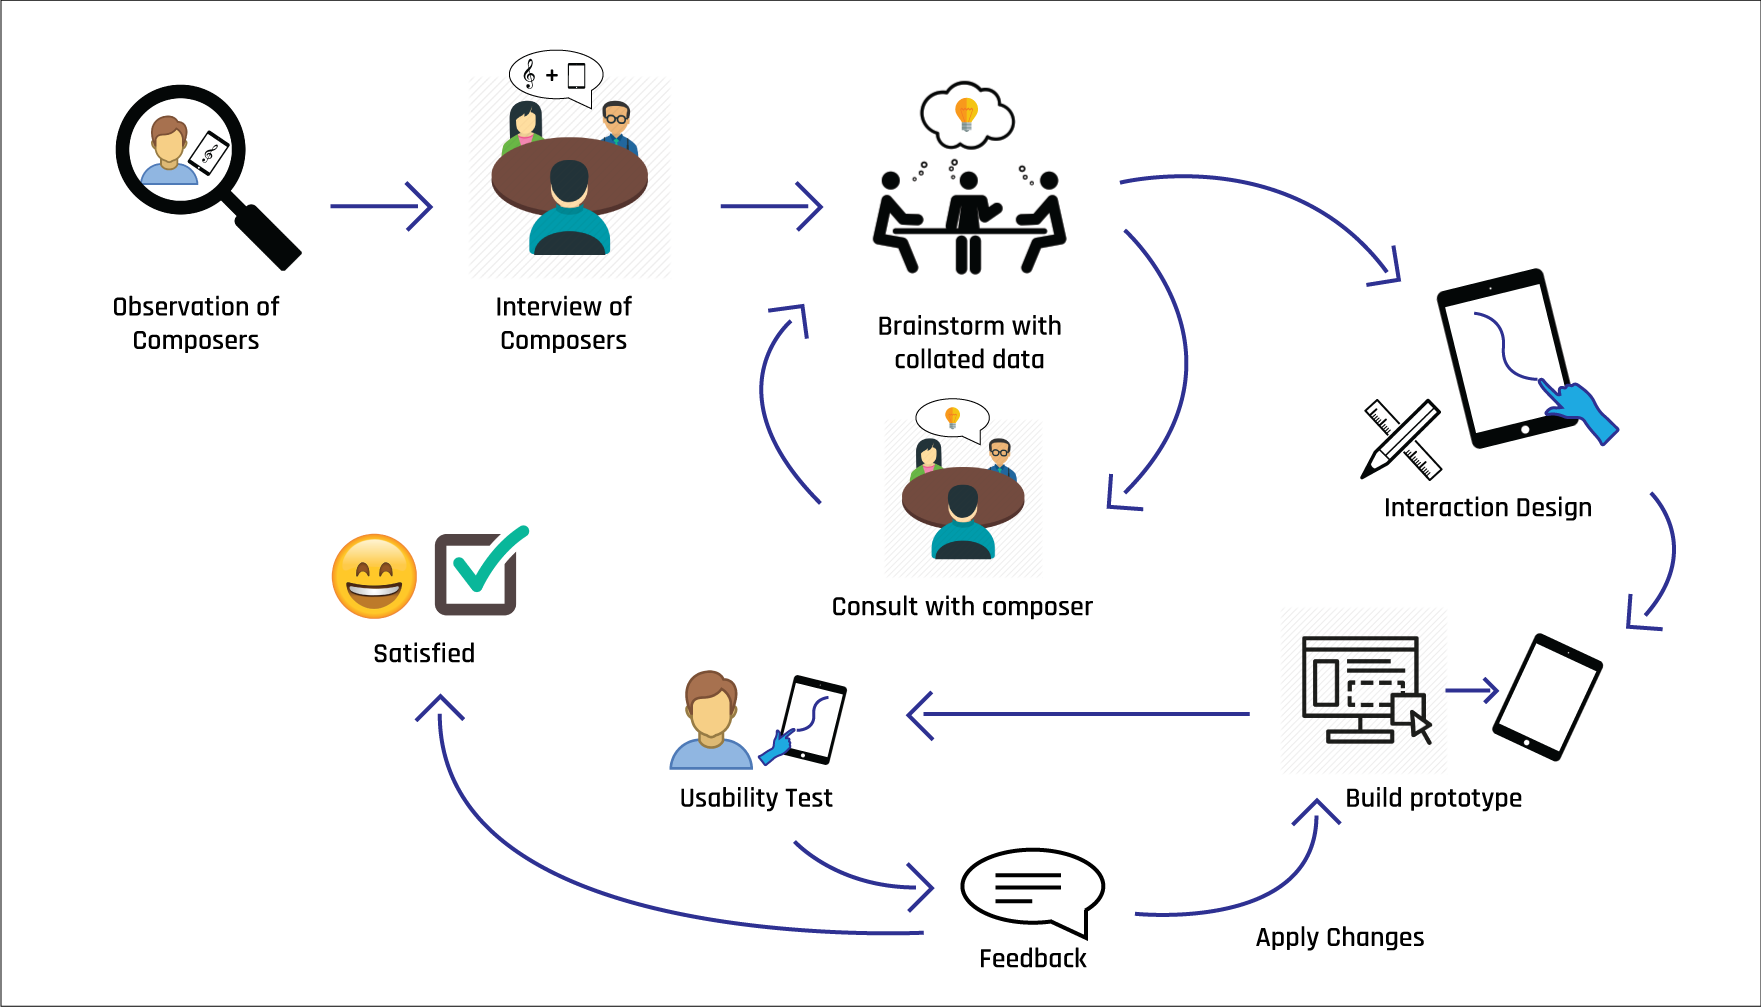
\includegraphics[scale=0.25]{Research_Framework}
    \caption{The research framework for Flow.}
    \label{fig:researchframework}
\end{figure}

This study was designed to be repetitive and iterative, to allow for continuous improvement of the system. User research and observation are important steps to understanding the behavior of users and figuring out their pain points. This is followed by interviews with composers to confirm and process the information gathered from user tests and interviews. The points that were given by the composers would then be used in the brainstorming phase to determine a suitable solution. The team will then consult with the researchers about the proposed solution to gather their insights about it. The brainstorming would then be repeated to improve on the solution followed by another consultation. This would be repeated until the team is satisfied with the solution.

The next phase would involve designing the interaction of the proposed solution. This would be followed by the prototype phase where a prototype would be built, tested, and improved repeatedly. Usability tests would be performed with different prototypes to create a good user experience. This phase would be repeated multiple times until the researchers are satisfied with the results of the tests.

% \section{System Architecture and Framework}
\section{System Description}

\subsection{System Overview}

The system will integrate music theory and user experience in an interface for musical composition. The composition process of composers will be observed and analyzed so that the system can be built to fit this process. The system will undergo multiple revisions based on the results of user testing. It will be built for the iOS, but will be optimized for the iPad. It will provide users an interface to create/edit, and view compositions. The user can make use of the system through an interface containing compositional activities like adding, editing, and deleting notes. Finally, the system will allow users to save their composition, which can be imported to a MusicXML format.

\subsection{System Objectives}

	\subsubsection{General Objective}
		
        To provide an interface that allows composers to perform basic and advanced musical composition tasks via gesture interactions on a mobile platform.

	\subsubsection{Specific Objectives}
    
    	Specifically, the system will allow users to do the following: 
          \begin{enumerate}
              \item View, create, edit, and delete their own compositions
              \item Move cursor through tap gesture or cursor movement interface
              \item Pan or zoom around the interface
              \item Move note menu and cursor movement interface
              \item Hide bottom menu
              \item Hear their compositions
              \item Set the key and time signature of their compositions
              \item Add, edit, and delete notes/rests through the note menu
              \item Add polyphonic notes/chords
              \item Transposing a note or group of notes
              \item Highlighting a single note or group of notes
              \item Add, remove, or change an accidental/ottava on a note or group of notes
              \item Add ties/slurs to notes
              \item Transpose/Retrograde a note or a group of notes
              \item Cut, copy, and paste a note/rest or a group of notes/rests
              \item Add or remove dots on a note or group of notes
              \item Undo/redo action
              \item Change composition tempo
              \item Input notes through the keyboard interface
              \item Playback composition
              \item Save the composition to be stored in local storage    

          \end{enumerate}
    
\subsection{Scope and Limitations of the System}

Given that the system is on a mobile platform, it would be limited in ability compared to that of desktop applications. This system aims to be a sketching application for composers that are on the go, or do not have their computers available. It will not contend with full-blown desktop musical composition applications like Finale or Sibelius.

Musical composition can be done for several kinds of instruments. However, the way music is composed varies from one instrument to another. With that said, the system will only support compositions for the piano. The system will also limit the musical notation symbols that can be used. The ones available for use are: 

\begin{itemize}
	\item Sixty-fourth note to whole note
    \item Sixty-fourth rest to whole rest
    \item Accidentals (sharp, flat, double-sharp)
\end{itemize}

Composers will also need to save their compositions in cases where they could not finish entirely and want to go back to it. A composition also has several elements which would be hard to model in databases. Thus, MusicXML will be used as the file format for saving data. This also makes it easy to transfer work from the system to other musical composition applications.

Gesture interactions are the main method of interaction within the system. Some gestures like tapping on the line need to be accurate and precise. To improve this precision, bigger screens will be needed. The iPad will be the best for this due to it having a large screen, yet still being portable. The testing will also be done on the iPad only.

Finally, the system's potential musical metacreation feature will need to have a model for generating the succeeding notes. To make it lightweight, the system will make use of a rule-based model similar to that of Computoser \citep{bozhanov2014computoser} and SuperWillow \citep{schulze2011music}. The model will take into account music theory for its rules.

\subsection{Data Design}

Given that musical compositions have a lot of elements which need to be stored as data, using relational databases for storage would prove to be inefficient and unintuitive \citep{hristidis2003efficient}. That is why the system would represent data through the use of MusicXML, which was also used in the SuperWillow system found in the study of \citeauthor{schulze2011music}.

MusicXML is a method of storing and representing digital sheet music through XML \citep{makemusic2017musicxml}. Because it is an Extensible Markup Language (XML), it follows a specific format that defines a logical structure \citep{bray1997extensible}, which in this case is a musical composition. The advantage of the MusicXML format is that it is used in several musical composition applications and can easily be shared between these applications \citep{makemusic2017musicxml}. Also, it can represent the most complicated aspects of musical notation like repeats, slurs, and more.

Shown in Table \ref{tab:musicxml} are the some of the commonly used elements and their respective descriptions in MusicXML.
 
\begin{longtable}{|p{3.6cm}|p{10cm}|} 
\caption{Commonly Used MusicXML Elements} \label{tab:musicxml} \\
\hline
       
       Element & Description \\ \hline
		
        \texttt{<score-partwise>} & Defines that the composition is divided into several parts, and these parts can have multiple measures. \\ \hline
        
        \texttt{<score-timewise>} & An alternative to the \texttt{<score-timewise>}, it defines the composition to have multiple measures where the measures can have many parts. \\ \hline

		\texttt{<part-list>} & Lists the parts of the composition. \\ \hline
        
        \texttt{<score-part>} & To be used as a child of \texttt{<part-list>}, this element adds a new part to the composition. Commonly supplied with the \texttt{id} attribute. \\ \hline
        
        \texttt{<part-name>} & A child of the \texttt{<score-part>} element, specifies the name of its parent part. \\ \hline
        
        \texttt{<attributes>} & Lists essential information in the composition such as the key, time signature, and clef. \\ \hline
        
        \texttt{<divisions>} &  Used in the production of sound. It works with the \texttt{<duration>} element to tell how many divisions per quarter note equal to the duration indicated. \\ \hline
        
        \texttt{<key>} & Denotes which key signature the composition is in and contains the \texttt{<fifths>} element. \\ \hline
        
        \texttt{<fifths>} & This element is derived from the circle of fifths and says how many sharps or flats the composition has. \\ \hline
        
        \texttt{<time>} & The time element contains information about the time signature which can be set using the \texttt{<beats>} and \texttt{<beat-type>} tags. \\ \hline
        
        \texttt{<beats>} & The numerator of the time signature. \\ \hline
        
        \texttt{<beat-type>} & The denominator of the time signature. \\ \hline
        
        \texttt{<clef>} & Tells the clef to be used in the composition through the \texttt{<sign>} and \texttt{<line>} tags. \\ \hline
        
        \texttt{<sign>} & Specifies the sign to be used for the clef.\\ \hline
        
        \texttt{<line>} & Specifies which line the set sign will start. \\ \hline
        
        \texttt{<note>} & Contains information inside that is needed to define a single note. \\ \hline
        
        \texttt{<pitch>} & Located inside the \texttt{<note>} element, it contains the \texttt{<step>} and \texttt{<octave>} elements that would indicate where the note would be placed. \\ \hline
        
        \texttt{<step>} & Indicates the pitch step. Must always be supplied in the \texttt{<pitch>} element. \\ \hline
        
        \texttt{<octave>} & Indicates the octave of the pitch. Also required. \\ \hline

        \texttt{<alter>} & An optional element in the \texttt{<pitch>} that indicates if the note has a sharp or flat. \\ \hline
        
        \texttt{<duration>} & Also an element inside the \texttt{<note>}, it works with the \texttt{<division>} element to denote what kind of note or sound it would play. \\ \hline
        
        \texttt{<type>} & Mainly serves to indicate how the note will be displayed or notated. \\ \hline


\end{longtable}

Whenever a user creates a composition and saves it in the application, a corresponding MusicXML will be generated and saved in the device's local storage. The MusicXML will be used to load the composition again, in case the user wants to edit or view it. 

\subsection{System Framework}

\begin{figure}[H]
	\centering
	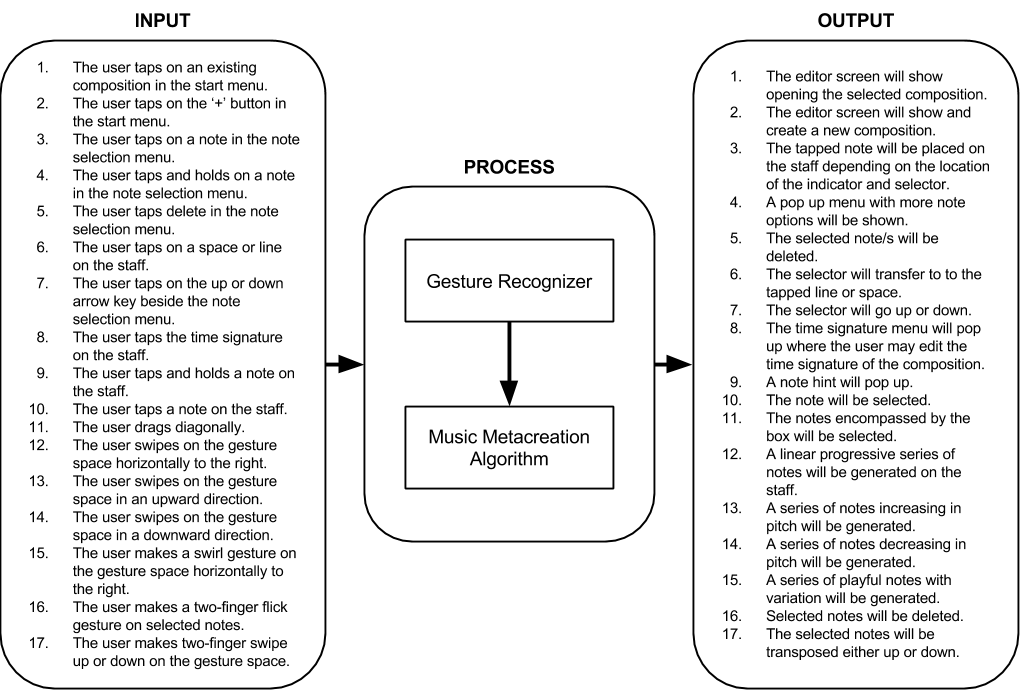
\includegraphics[scale=0.4]{System_Framework}
    \caption{The system framework for Flow.}
    \label{fig:systemframework}
\end{figure}

The system framework, shown in Figure \ref{fig:systemframework}, illustrates an overview of how Flow works. Input is relatively simple, mainly in the form of gestures. Users can tap, swipe, hold, or drag on specific objects. The application's gesture recognizer would then analyze the gesture performed by the user. The system would then output or perform the specific action assigned to each gesture. However, if the gesture is tied to musical metacreation, the application would output a set of notes based on its built-in algorithm.

\subsection{System Walkthrough}

\subsubsection{Main Menu}
The Main Menu (Figure \ref{fig:main-menu}) is the first screen shown to the user upon opening the application. This screen is where the user can create, open, export, and delete a composition. 

\subsubsection{Creating a Composition}
To create a new composition, the user may tap on the '+' icon which will lead to the Editor screen. 

\begin{figure}[H]
	\centering
	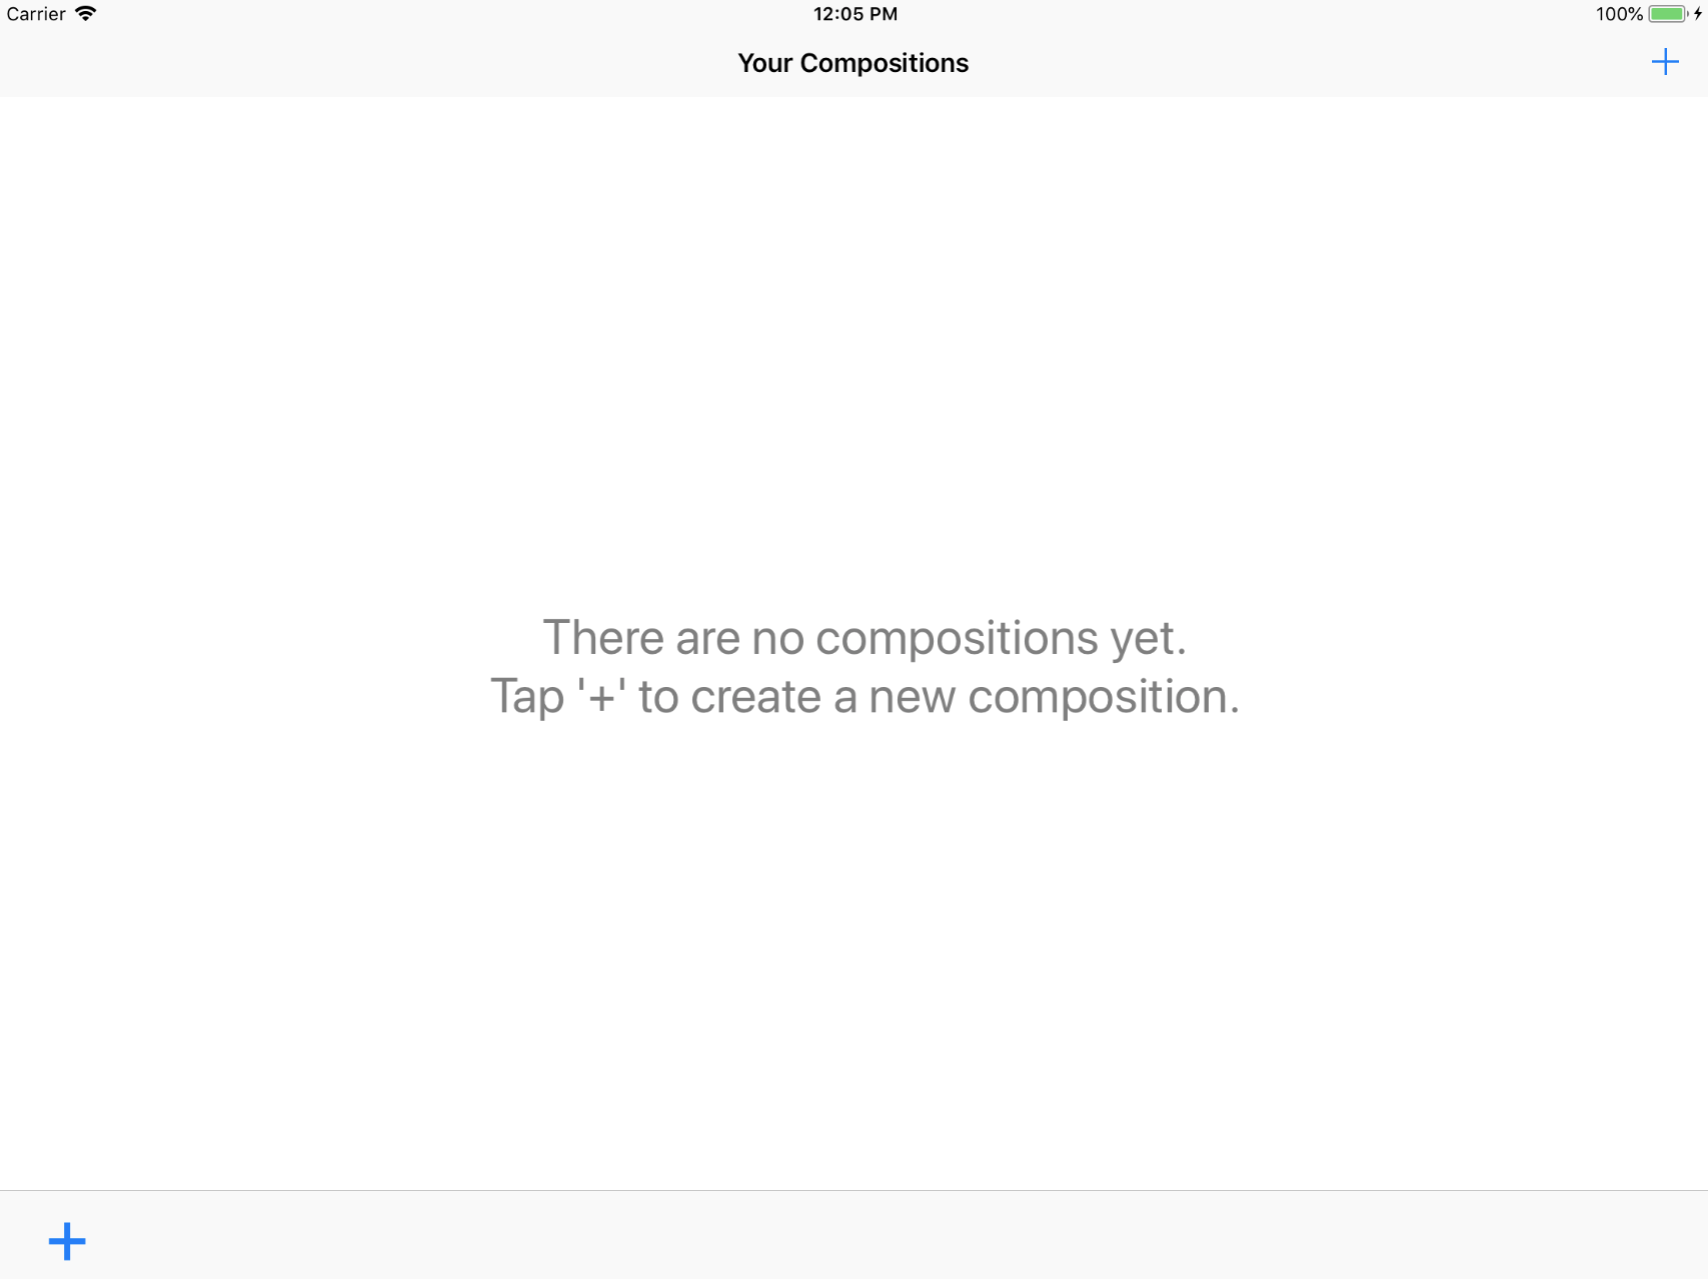
\includegraphics[scale=0.4]{Main_Menu}
    \caption{Flow Main Menu.}
    \label{fig:main-menu}
\end{figure}

\subsubsection{Opening a Composition}
Tapping an existing composition in the list will open it in the Editor screen allowing the user to edit. 

\subsubsection{Deleting, Renaming, and Exporting a Composition}
Swiping a composition to the left brings out the delete button (Figure \ref{fig:swipe-delete}). The user may also tap and hold an existing composition which brings out a modal for exporting (share), renaming, and deleting a composition (Figure \ref{fig:tap-hold-comp}).

\begin{figure}[H]
	\centering
	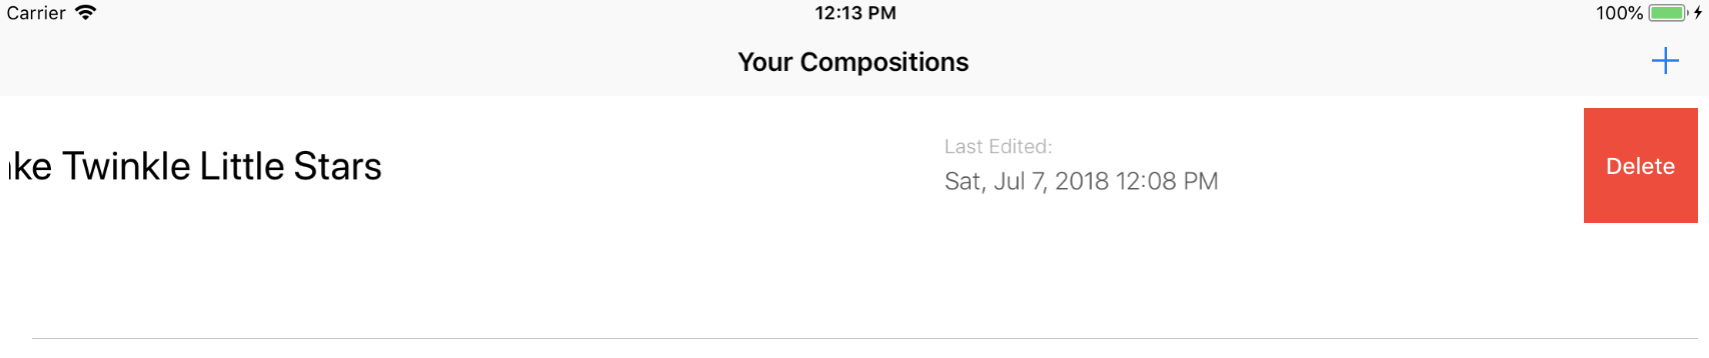
\includegraphics[scale=0.45]{Swipe_Delete}
    \caption{Swipe left to delete a composition.}
    \label{fig:swipe-delete}
\end{figure}

\begin{figure}[H]
	\centering
	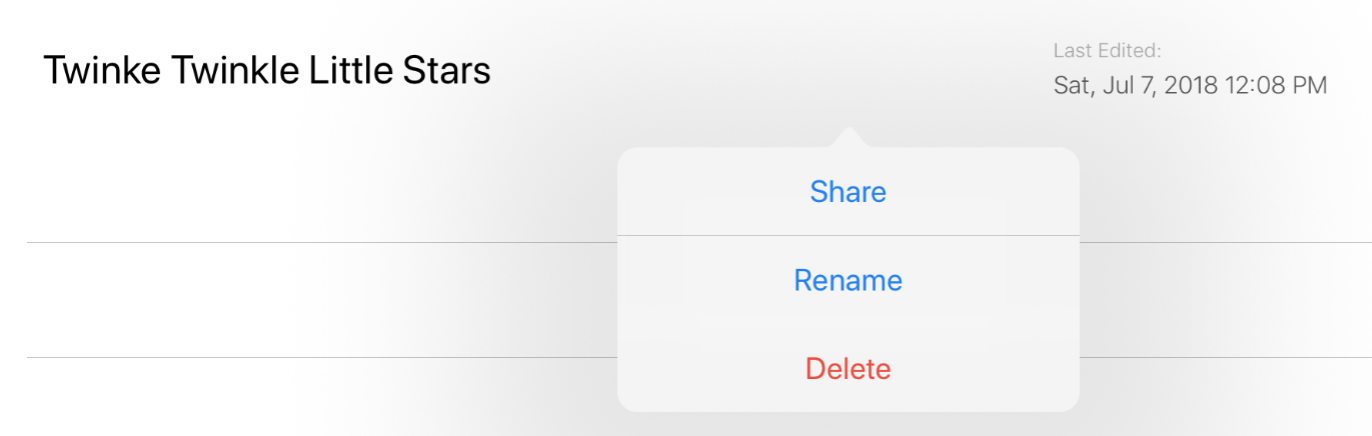
\includegraphics[scale=0.45]{Tap_And_Hold_Comp}
    \caption{Tap and hold a composition to bring out modal.}
    \label{fig:tap-hold-comp}
\end{figure}

\subsubsection{Editor}

The editor screen is where the user will spend most of the time using the application. It is where most of the composition process will take place. This includes adding, editing, and deleting of notes, rests and accidentals, setting the title, key signature, time signature, and tempo of the composition. This is also where the user can listen to the current progress of a composition through the playback functionality and also save a composition. Shown in Figure \ref{fig:editor} is the editor screen after creating a new composition from the main menu. 

\begin{figure}[H]
	\centering
	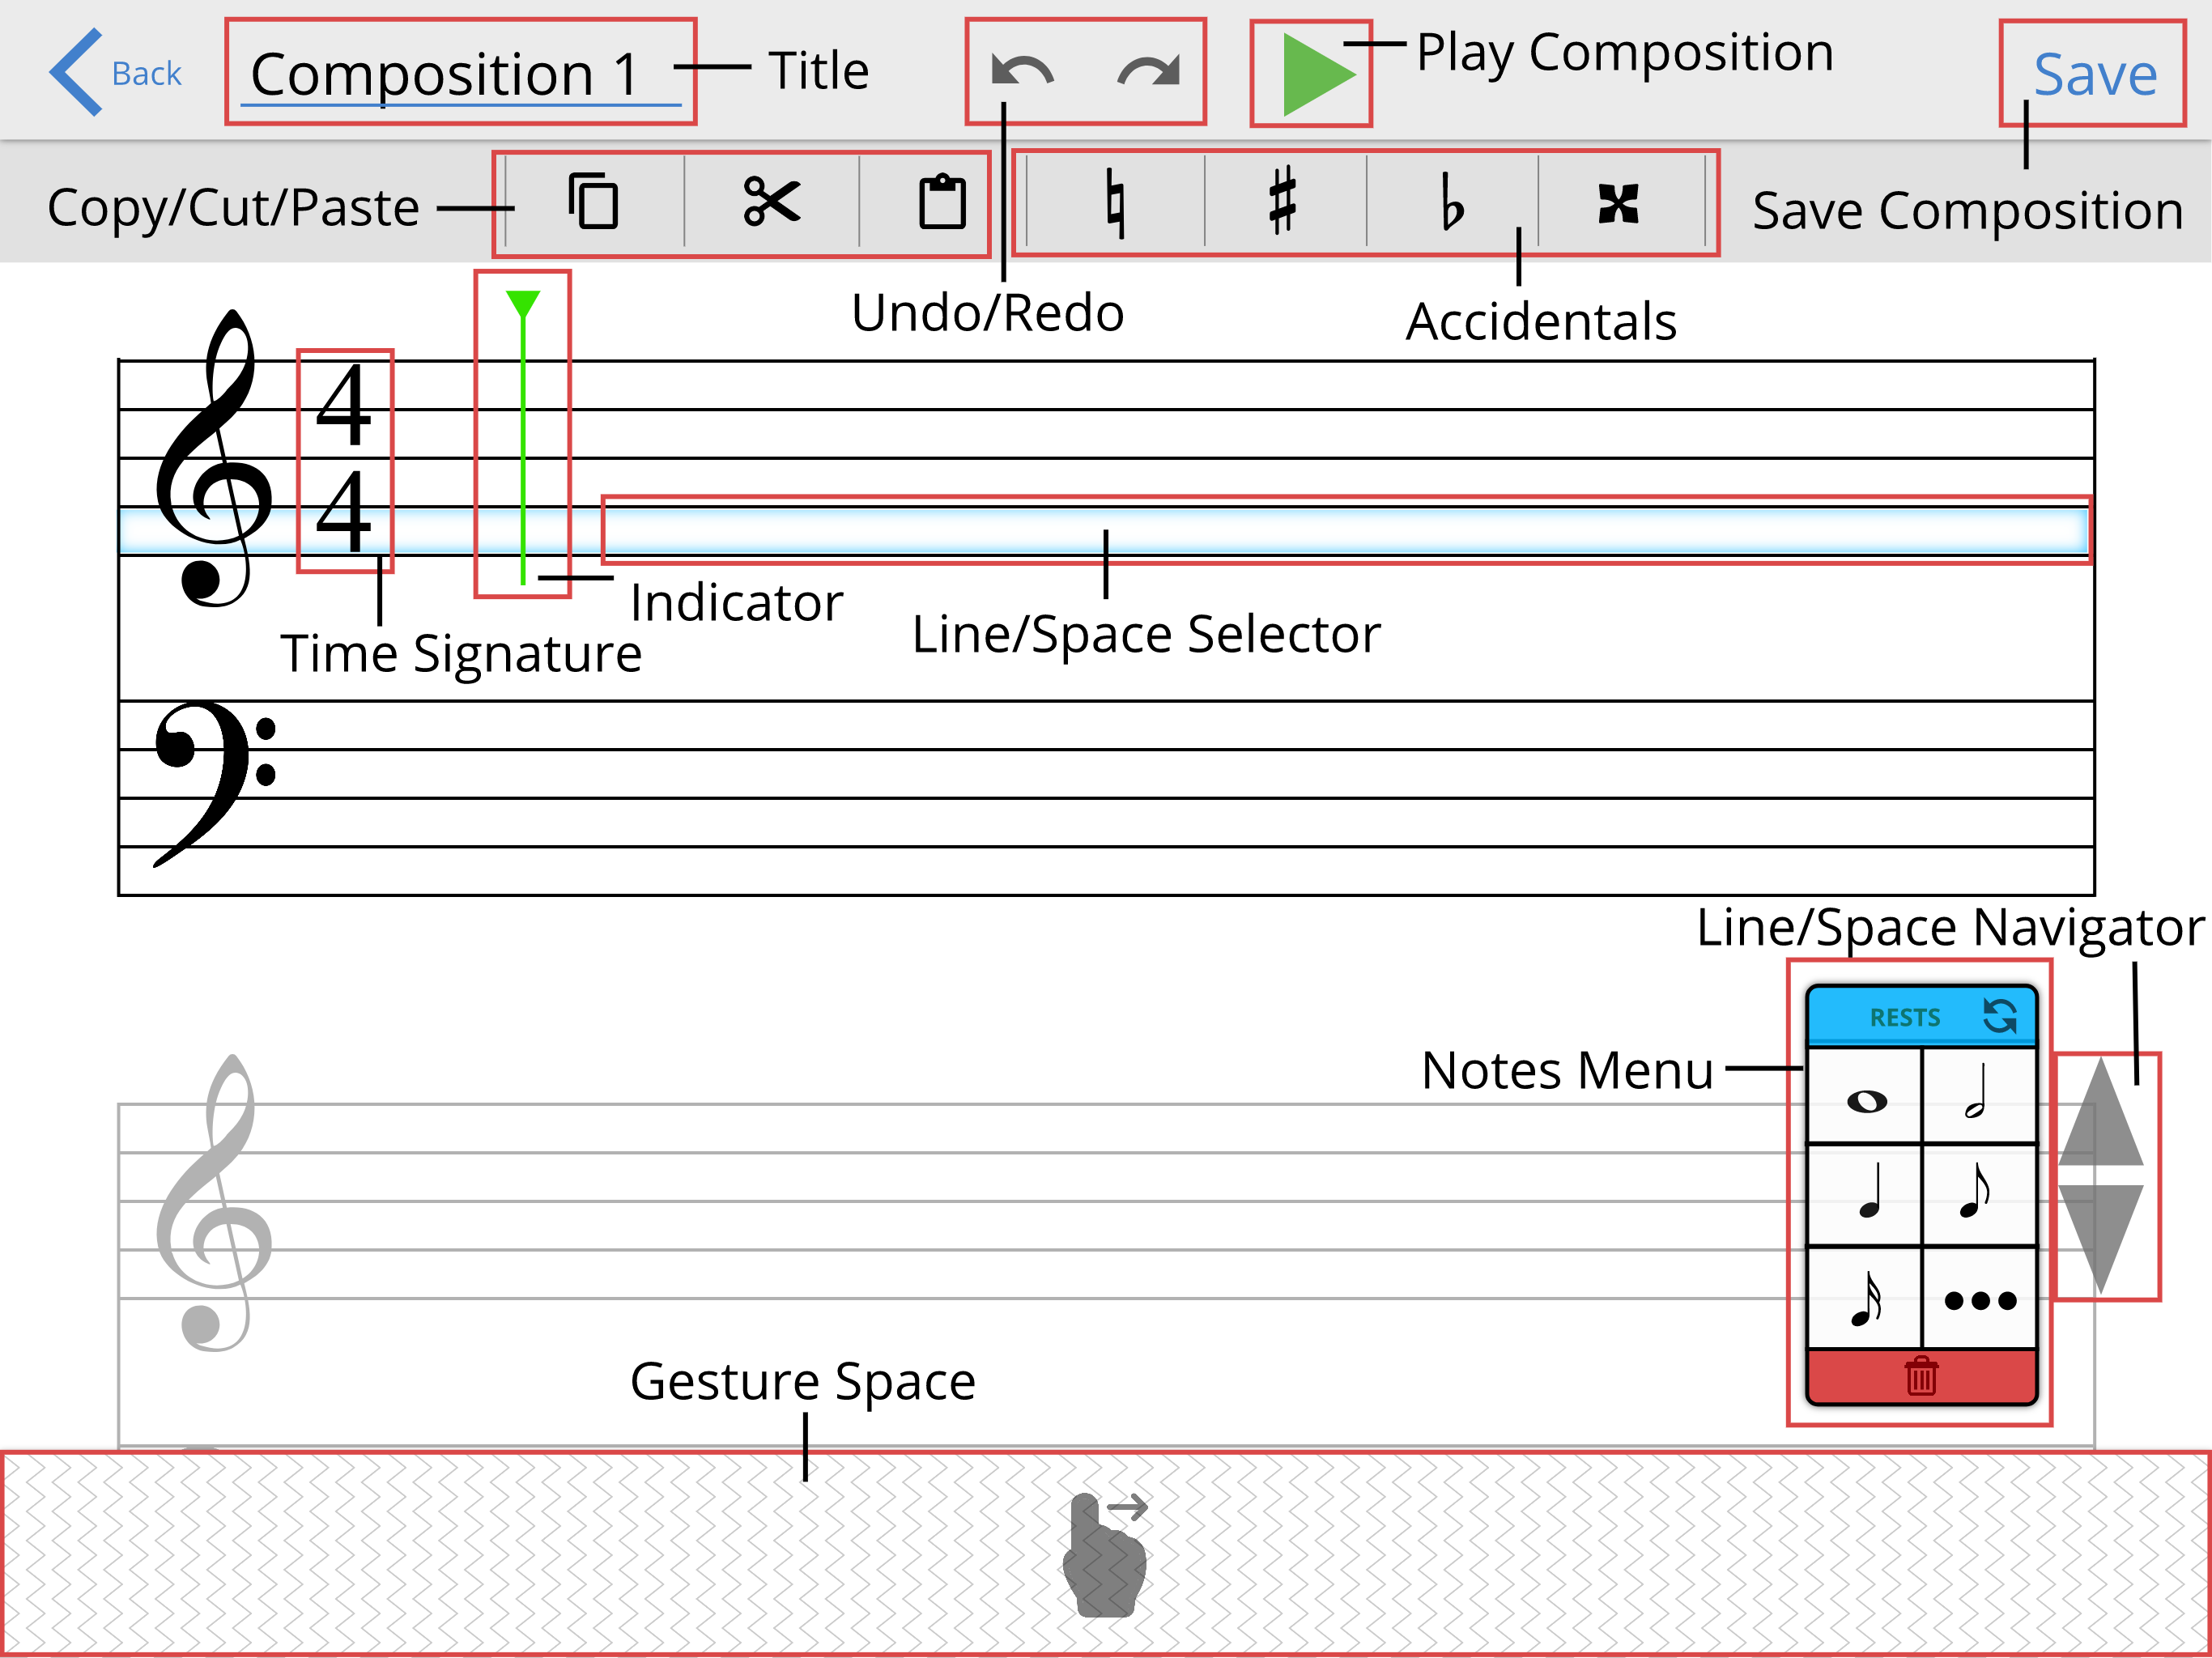
\includegraphics[scale=0.45]{Editor}
    \caption{Editor Screen.}
    \label{fig:editor}
\end{figure}

\subsubsection{Zooming and Panning}
To zoom out on the editor, the user must use the pinch in gesture (Figure \ref{fig:pinch-in}) and to zoom in, the user must use the pinch out gesture (Figure \ref{fig:pinch-out}). To pan the editor, the user must do a 2 finger drag gesture.

\begin{figure}[H]
	\centering
	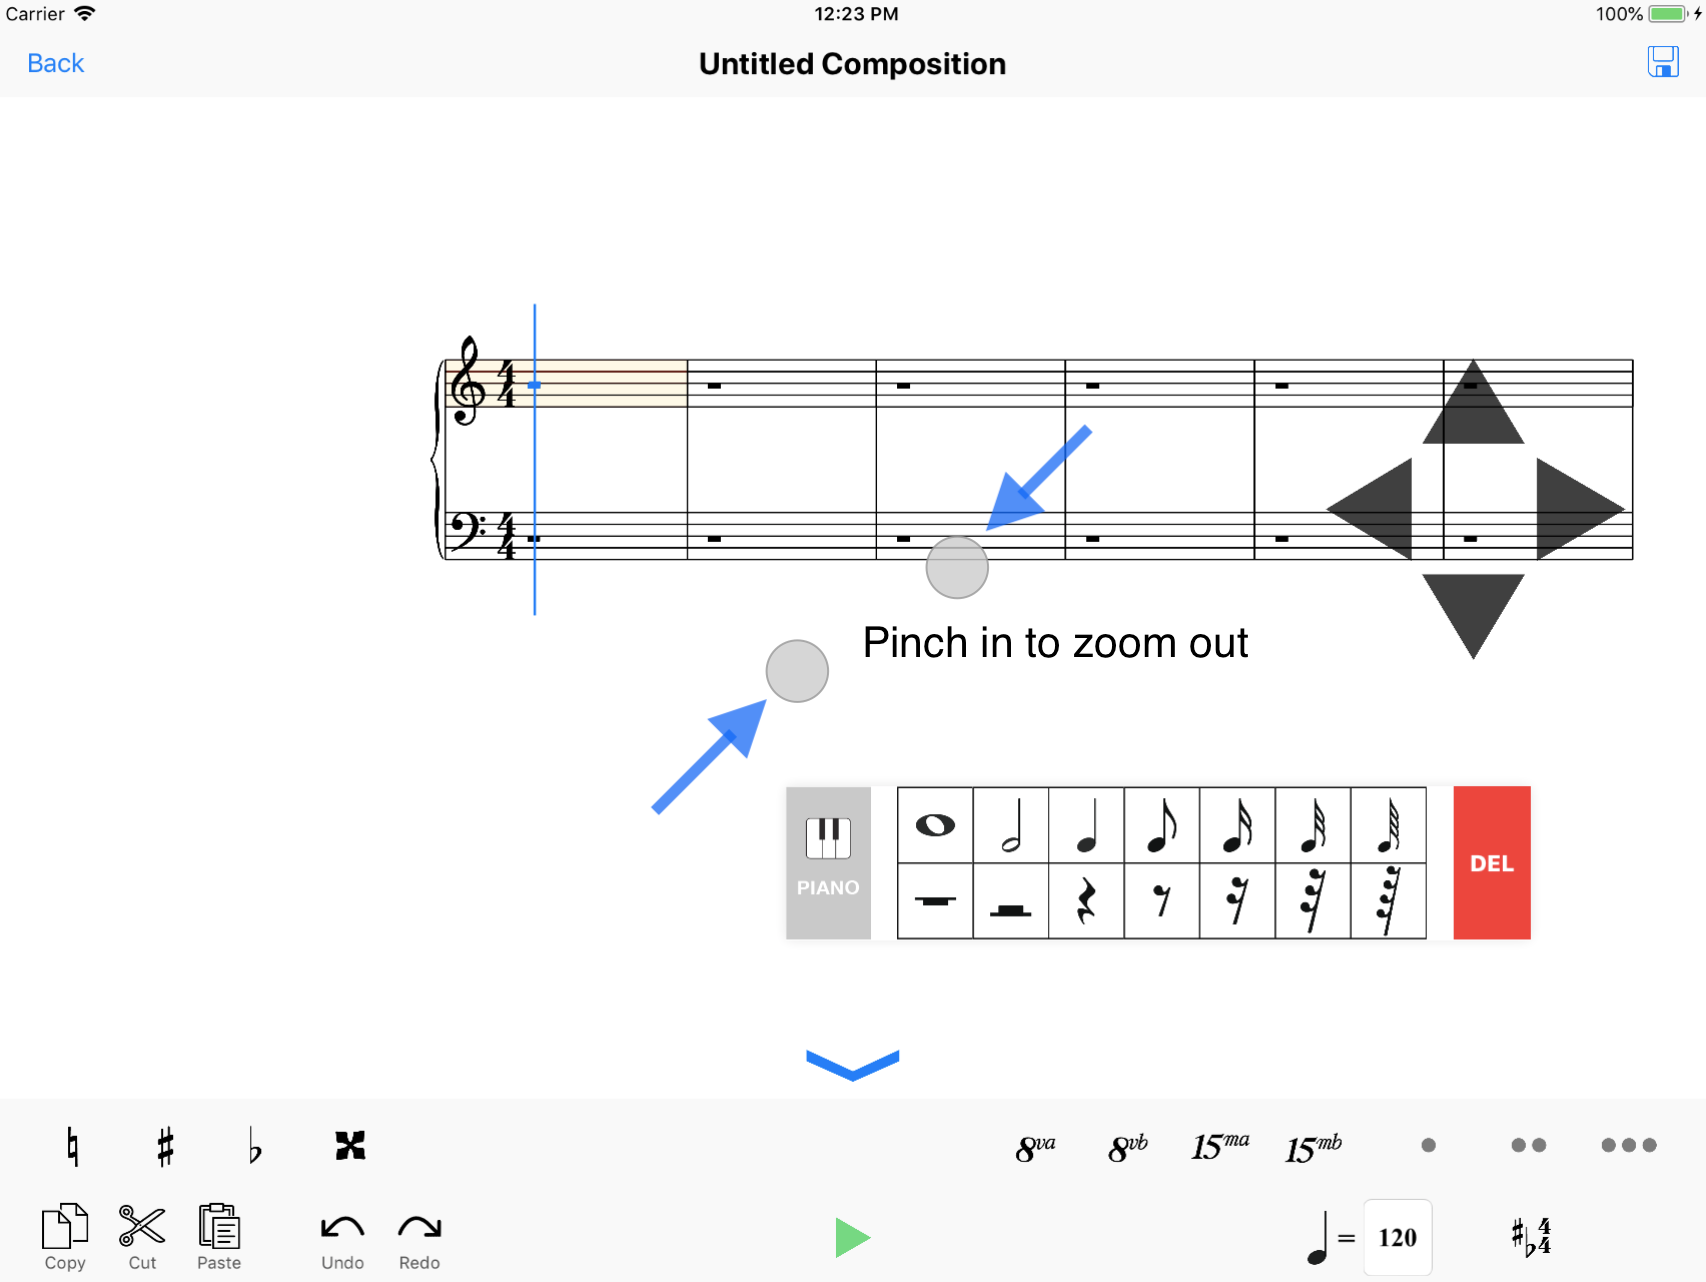
\includegraphics[scale=0.4]{Pinch_In}
    \caption{Pinch in to zoom out.}
    \label{fig:pinch-in}
\end{figure}

\begin{figure}[H]
	\centering
	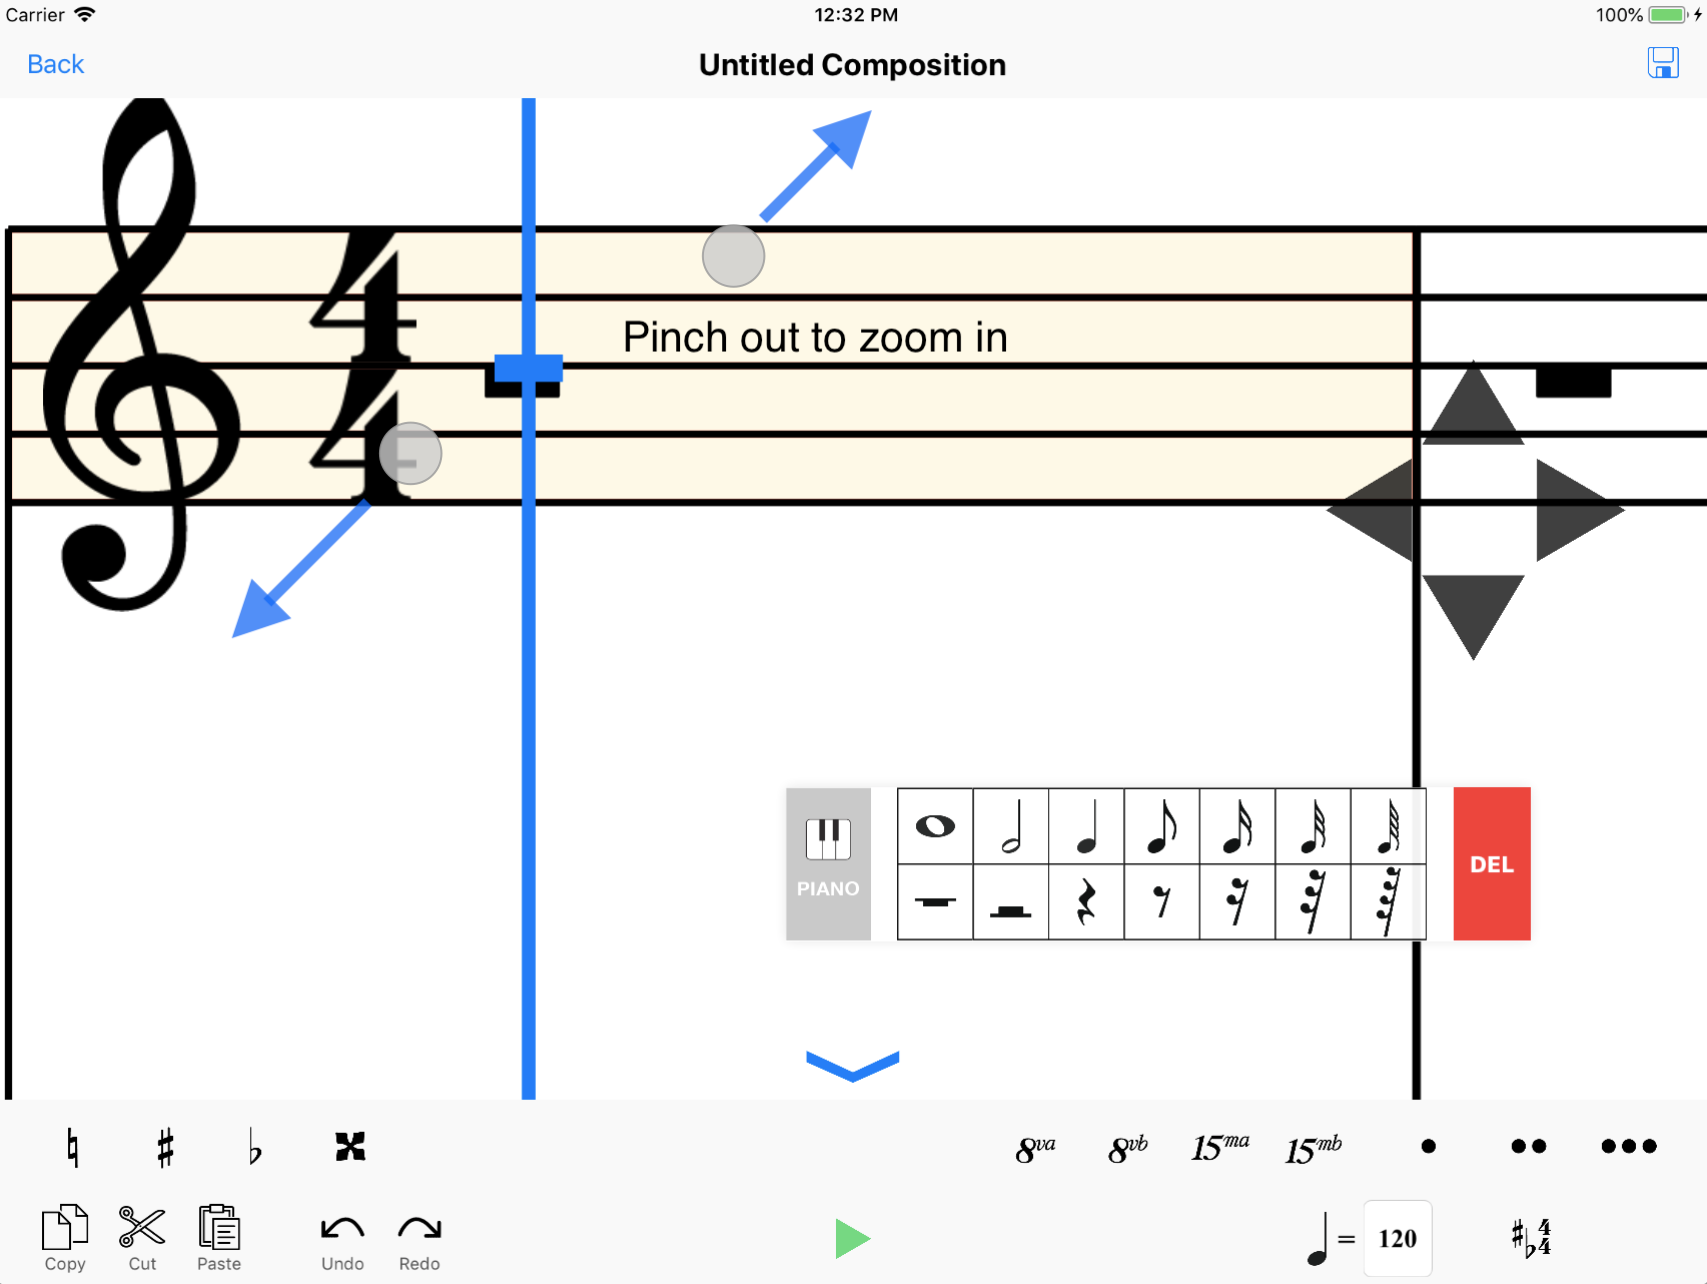
\includegraphics[scale=0.4]{Pinch_Out}
    \caption{Pinch out to zoom in.}
    \label{fig:pinch-out}
\end{figure}

\begin{figure}[H]
	\centering
	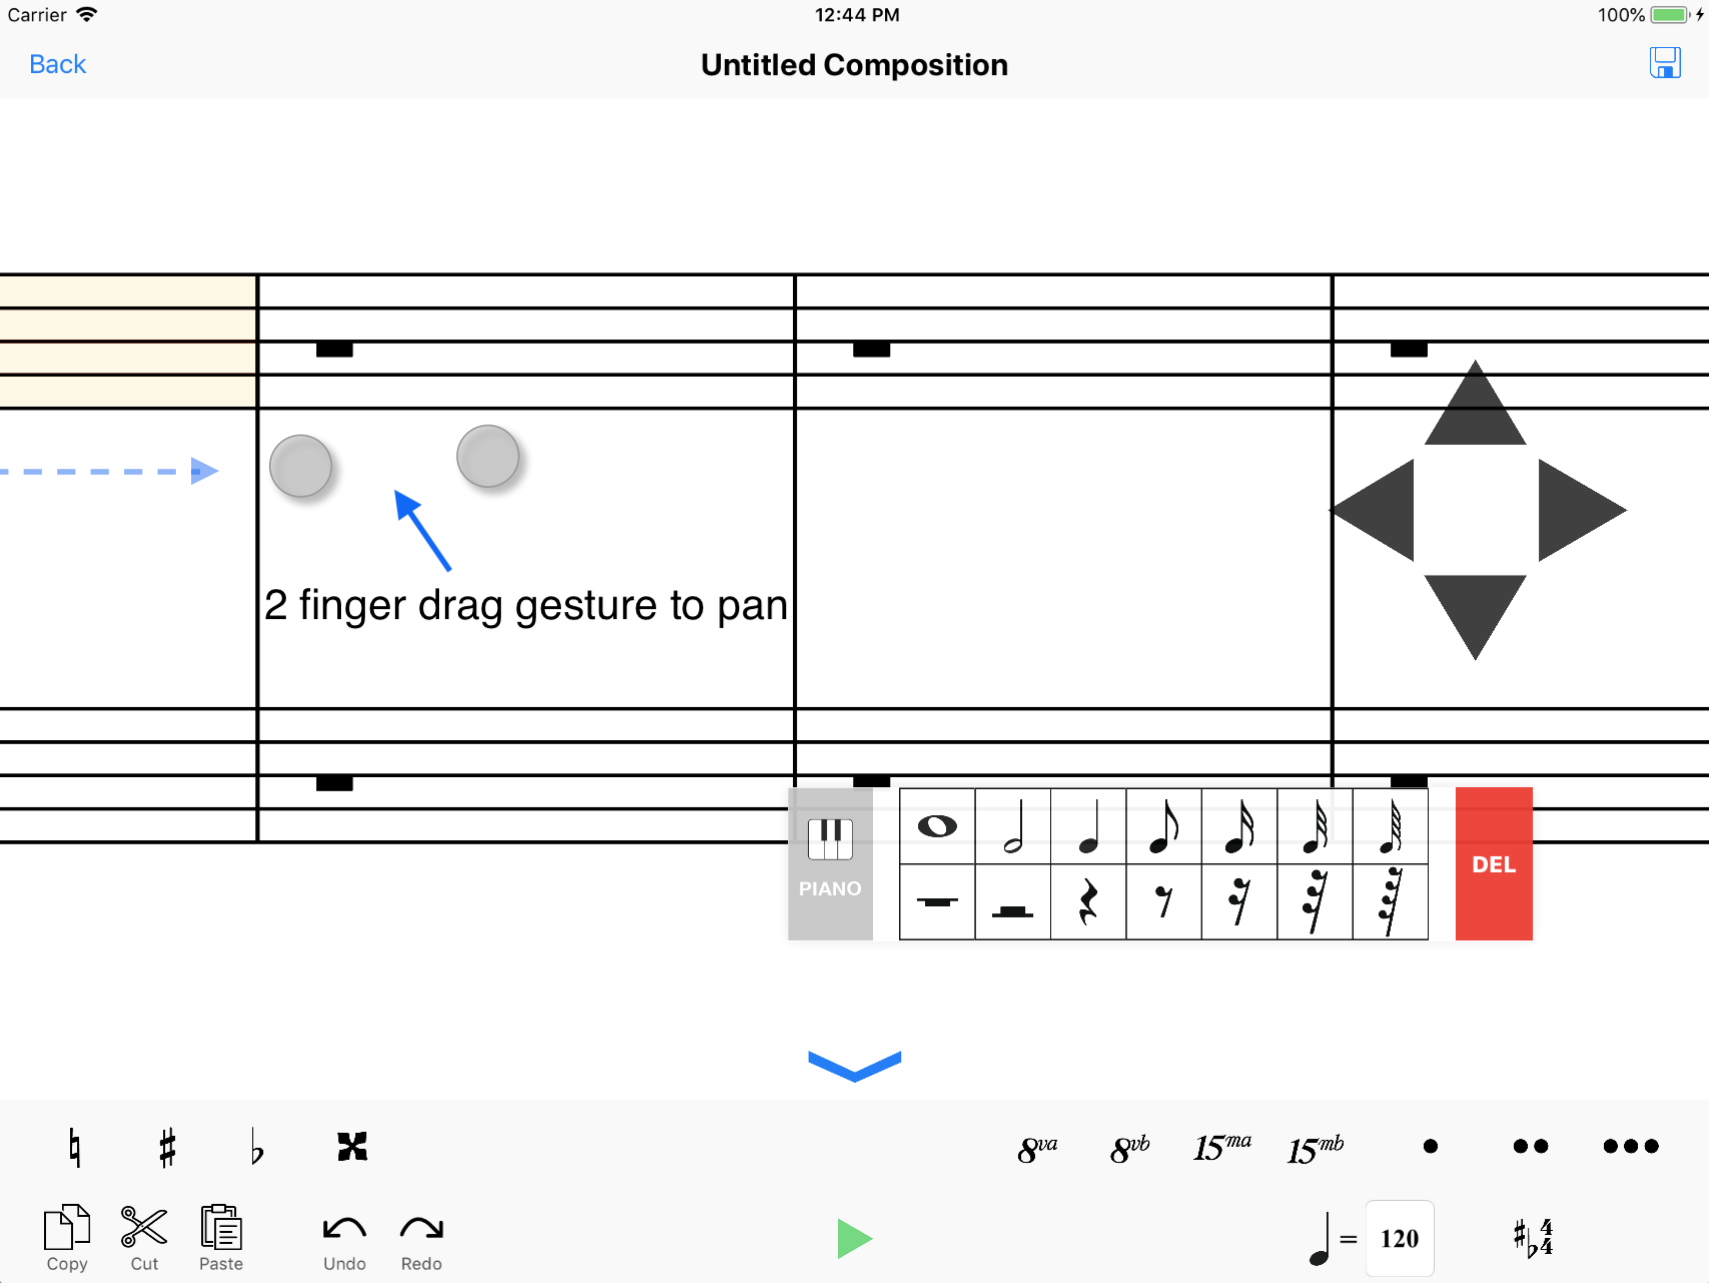
\includegraphics[scale=0.4]{Pan}
    \caption{Two finger drag gesture to pan.}
    \label{fig:pan}
\end{figure}

\subsubsection{Moving the Controls}
The controls in the editor such as the arrow controls and the notation controls are draggable views which allow the user to move them around for flexibility through a 1 finger drag gesture (Figure \ref{fig:move-controls}).

\begin{figure}[H]
	\centering
	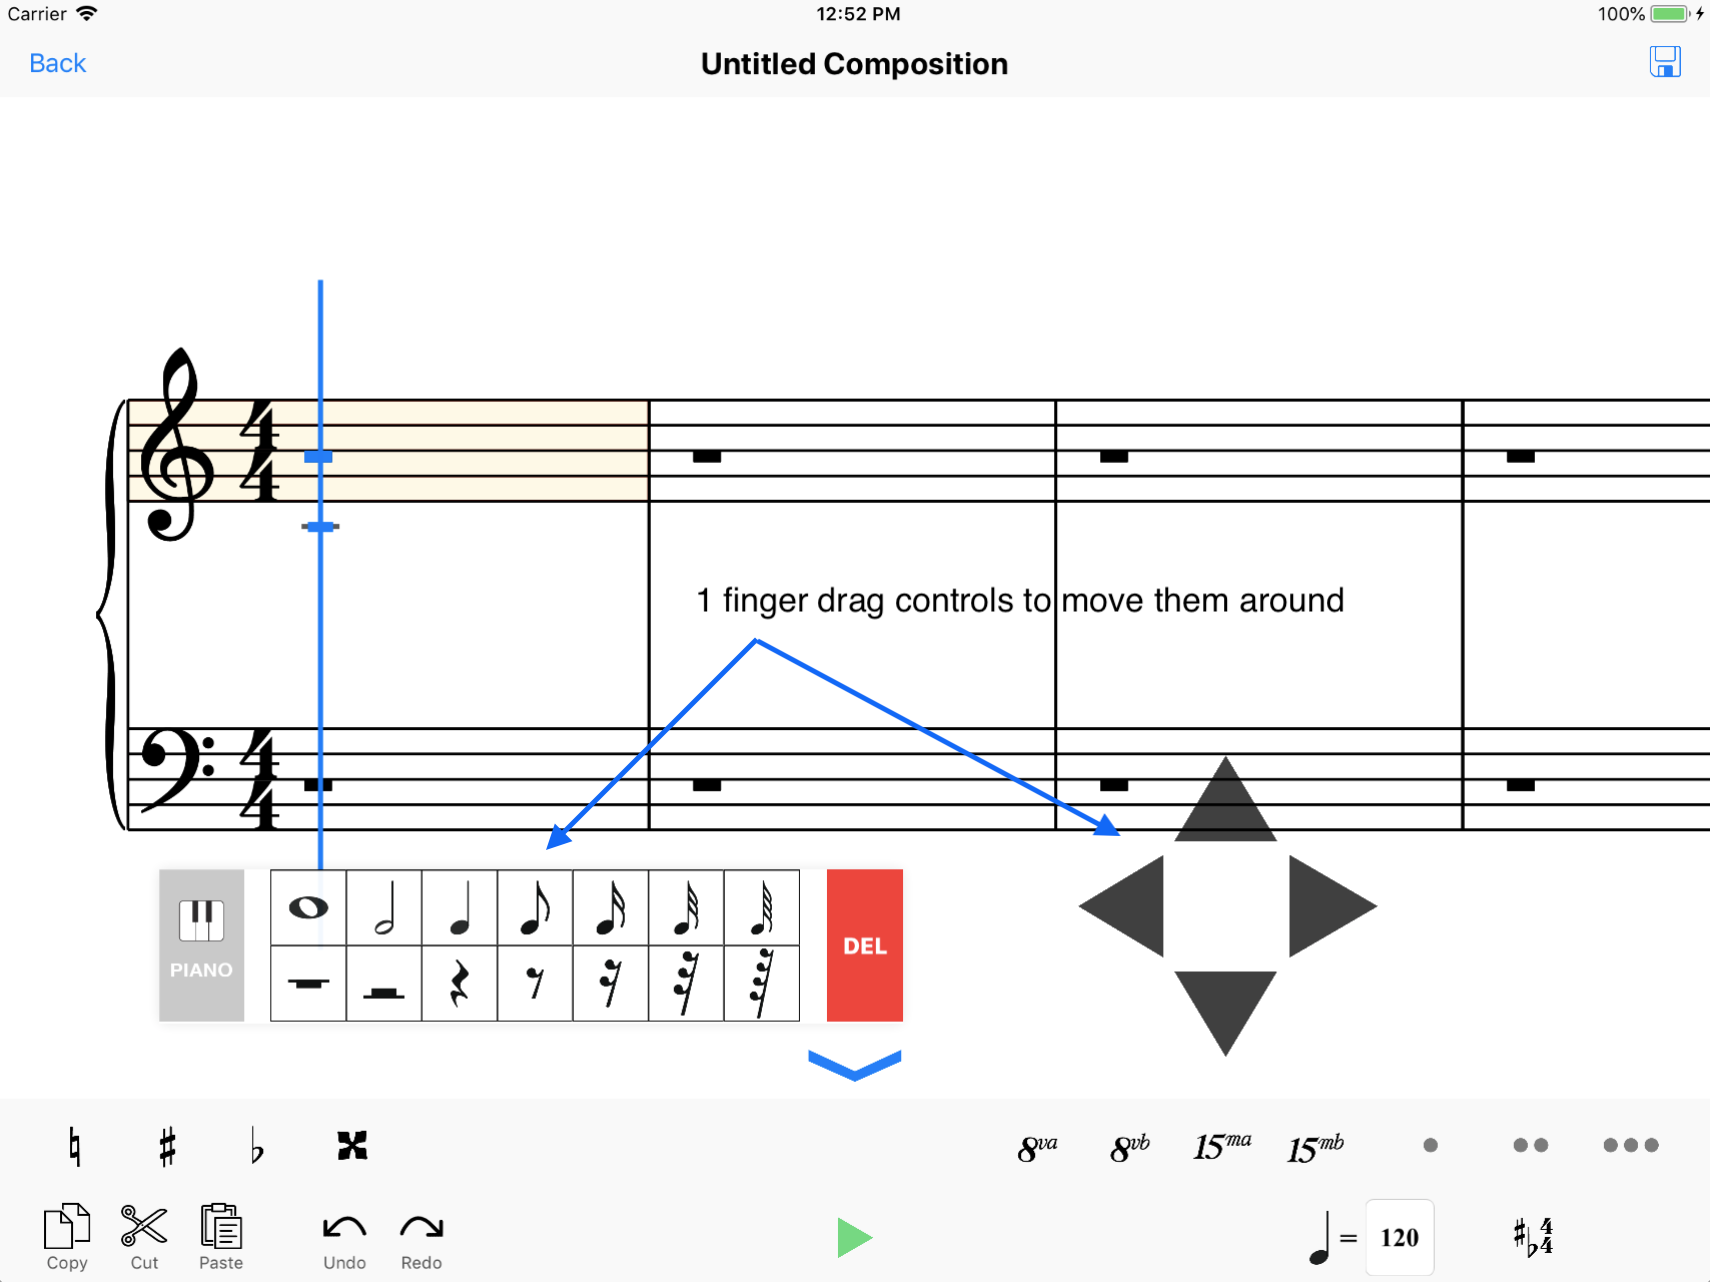
\includegraphics[scale=0.4]{Move_Controls}
    \caption{One finger drag gesture to move controls.}
    \label{fig:move-controls}
\end{figure}

\subsubsection{Renaming a Composition}
Initially, the title of a new composition is set to "Untitled Composition", and the user may edit it by tapping on the title text above in the application toolbar. 

\begin{figure}[H]
	\centering
	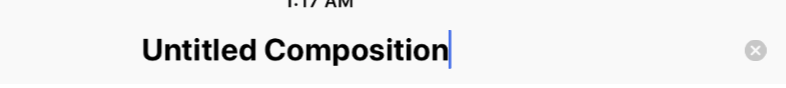
\includegraphics[scale=0.7]{Renaming}
    \caption{Renaming a composition.}
    \label{fig:renaming}
\end{figure}

\subsubsection{Moving the Cursor}
The blue cursor indicates where the next note or rest will be placed, and it also indicates the selected measure and the selected note or rest. There are currently three ways on how the user may move the blue cursor in the editor. The first way is through the use of the arrow controls. Tapping on the up or down arrow keys will change the pitch of the cursor either higher or lower by a half step (Figure \ref{fig:move-arrow-up}). Tapping on the left and right arrow keys, on the other hand, will move the selection of the cursor either to the previous or next note (Figure \ref{fig:move-arrow-right}). The second way of moving the cursor is by dragging it. Upon dragging the cursor, the horizontal line will elongate which indicates that the cursor is already being dragged by the user and also for the user to easily see the current location of the cursor (Figure \ref{fig:cursor-drag}). The third way is by tapping on a location in the editor. Doing so will automatically move the cursor on the tapped location (Figure \ref{fig:cursor-tap}).

\begin{figure}[H]
	\centering
	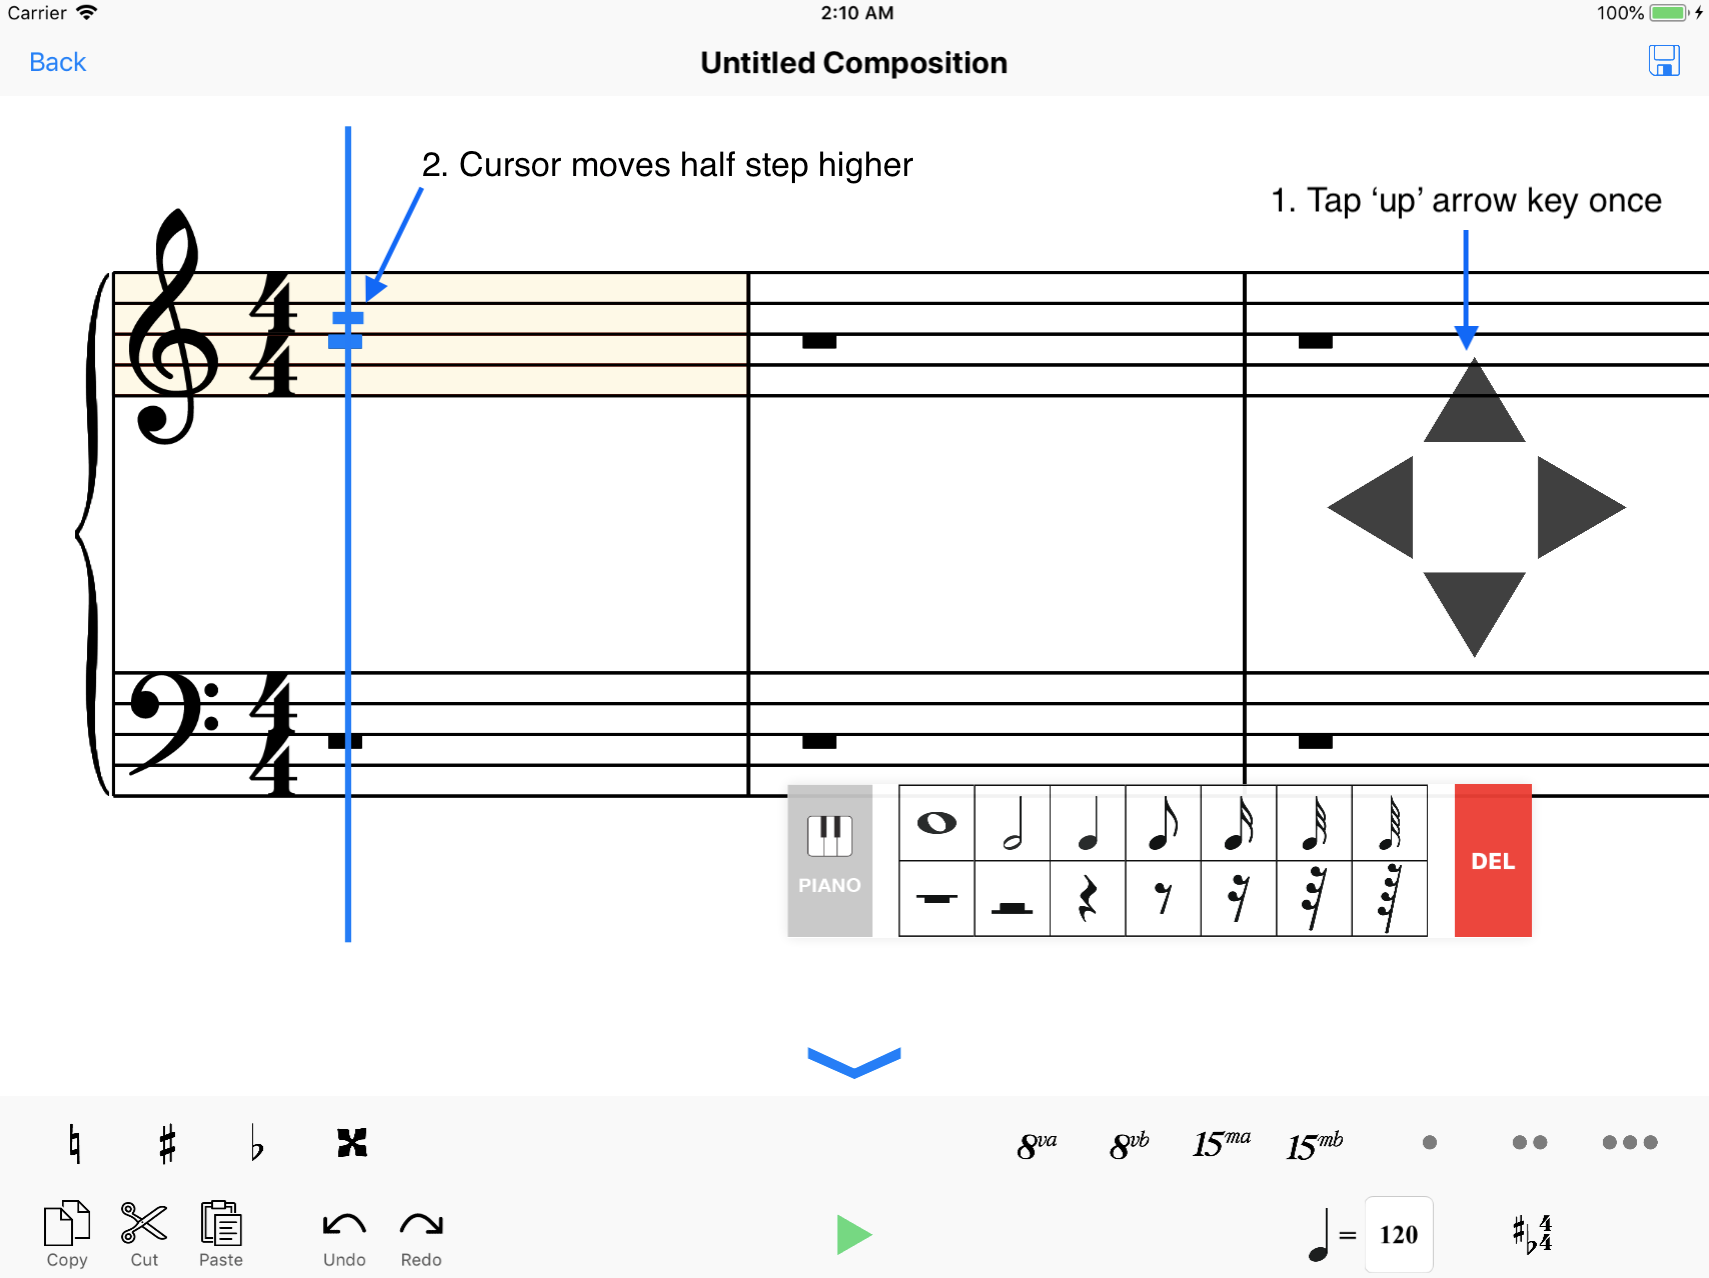
\includegraphics[scale=0.5]{Move_Arrow_Up}
    \caption{Move cursor by a half step higher.}
    \label{fig:move-arrow-up}
\end{figure}

\begin{figure}[H]
	\centering
	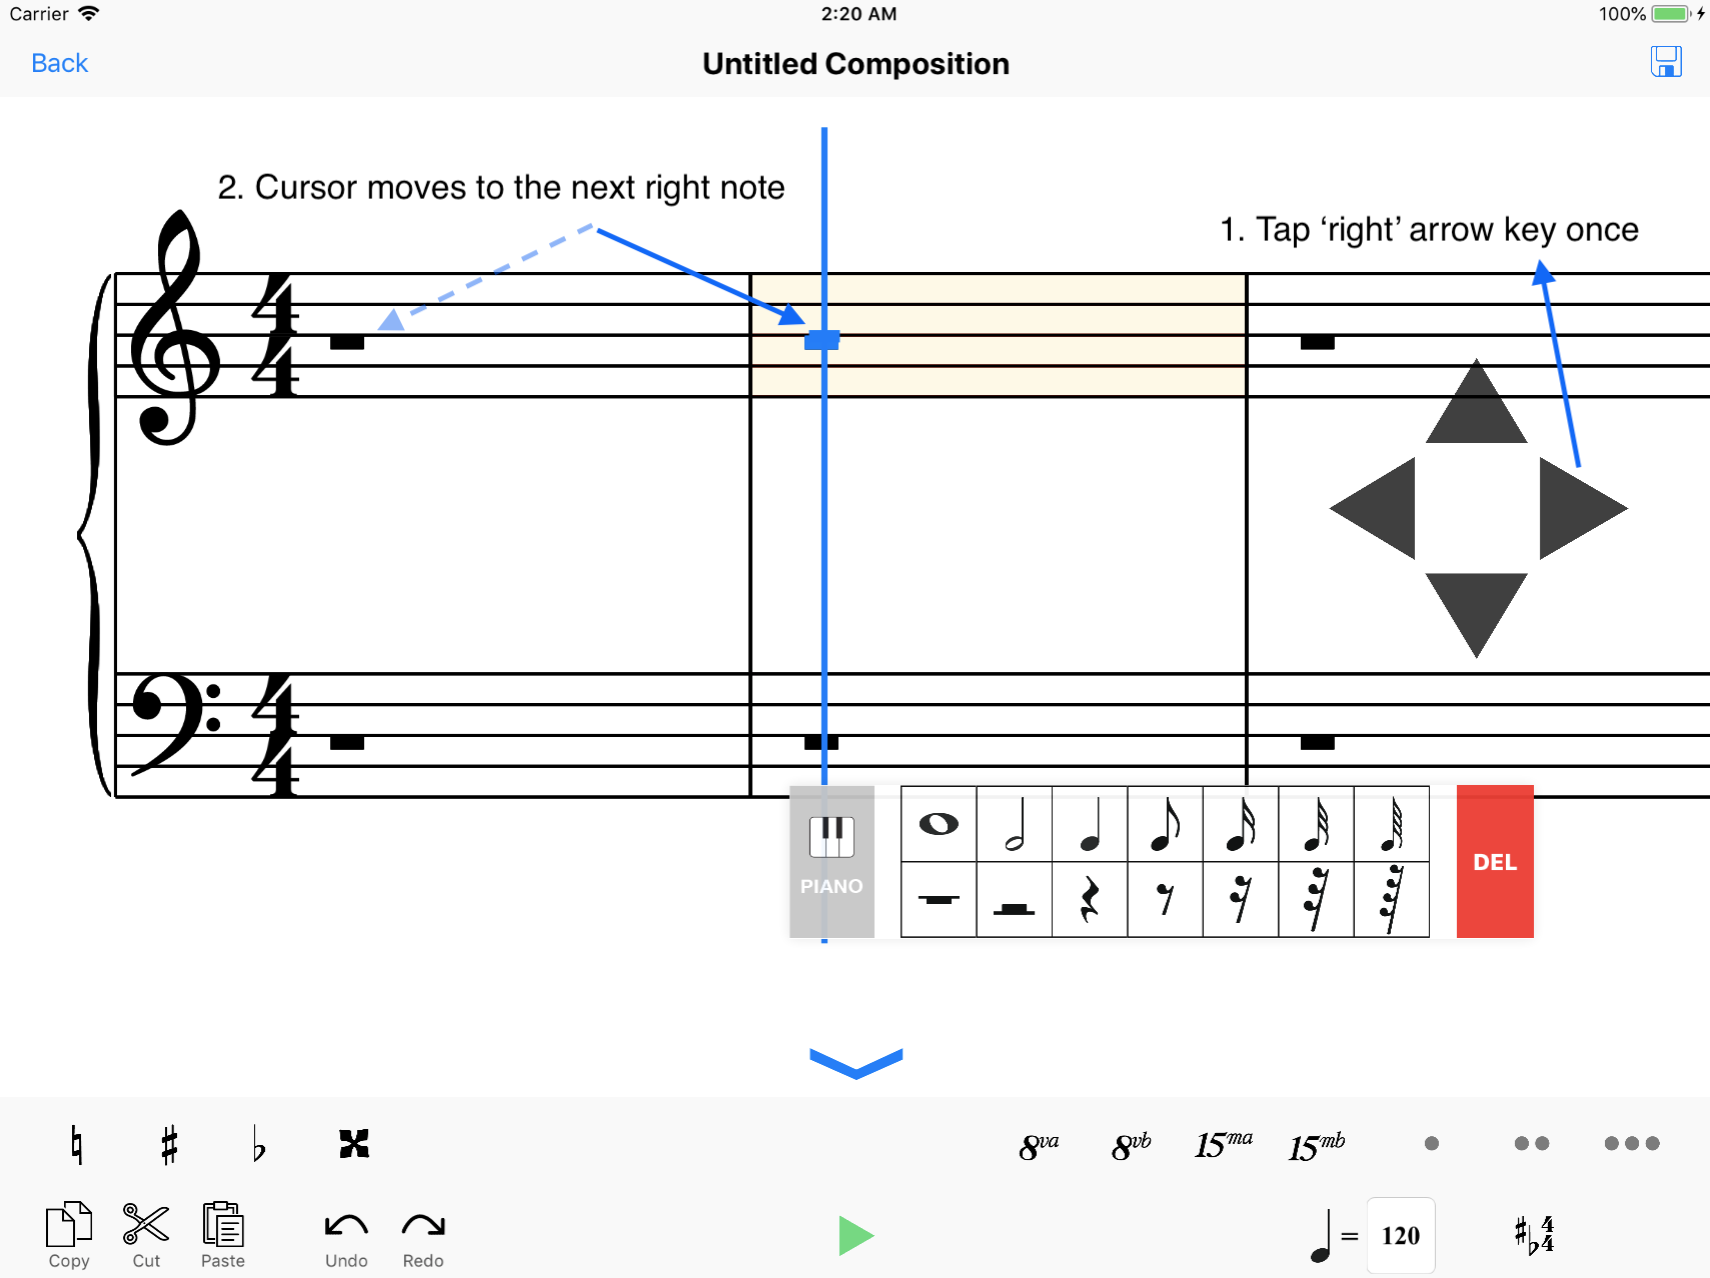
\includegraphics[scale=0.4]{Move_Arrow_Right}
    \caption{Move cursor next note to the right.}
    \label{fig:move-arrow-right}
\end{figure}

\begin{figure}[H]
	\centering
	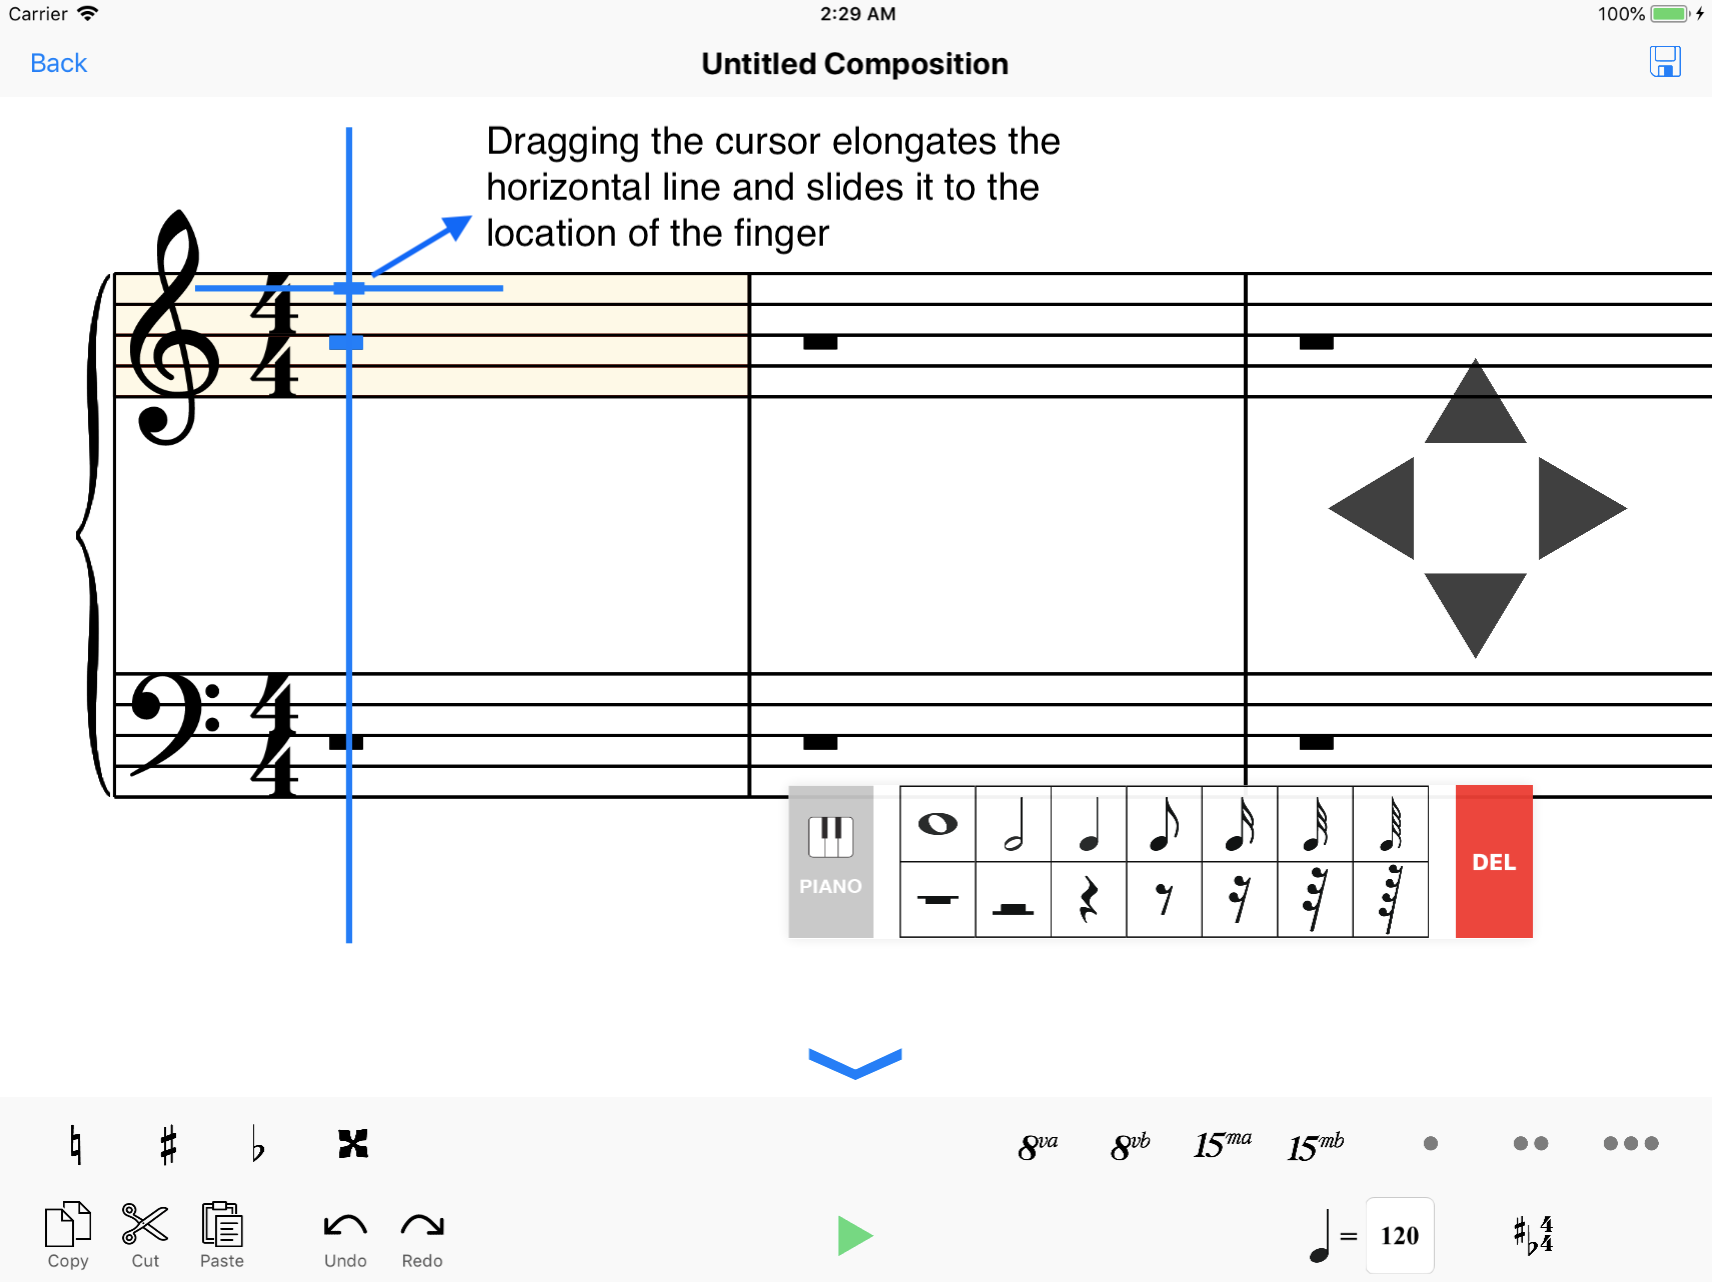
\includegraphics[scale=0.4]{Cursor_Drag}
    \caption{Dragging a cursor.}
    \label{fig:cursor-drag}
\end{figure}

\begin{figure}[H]
	\centering
	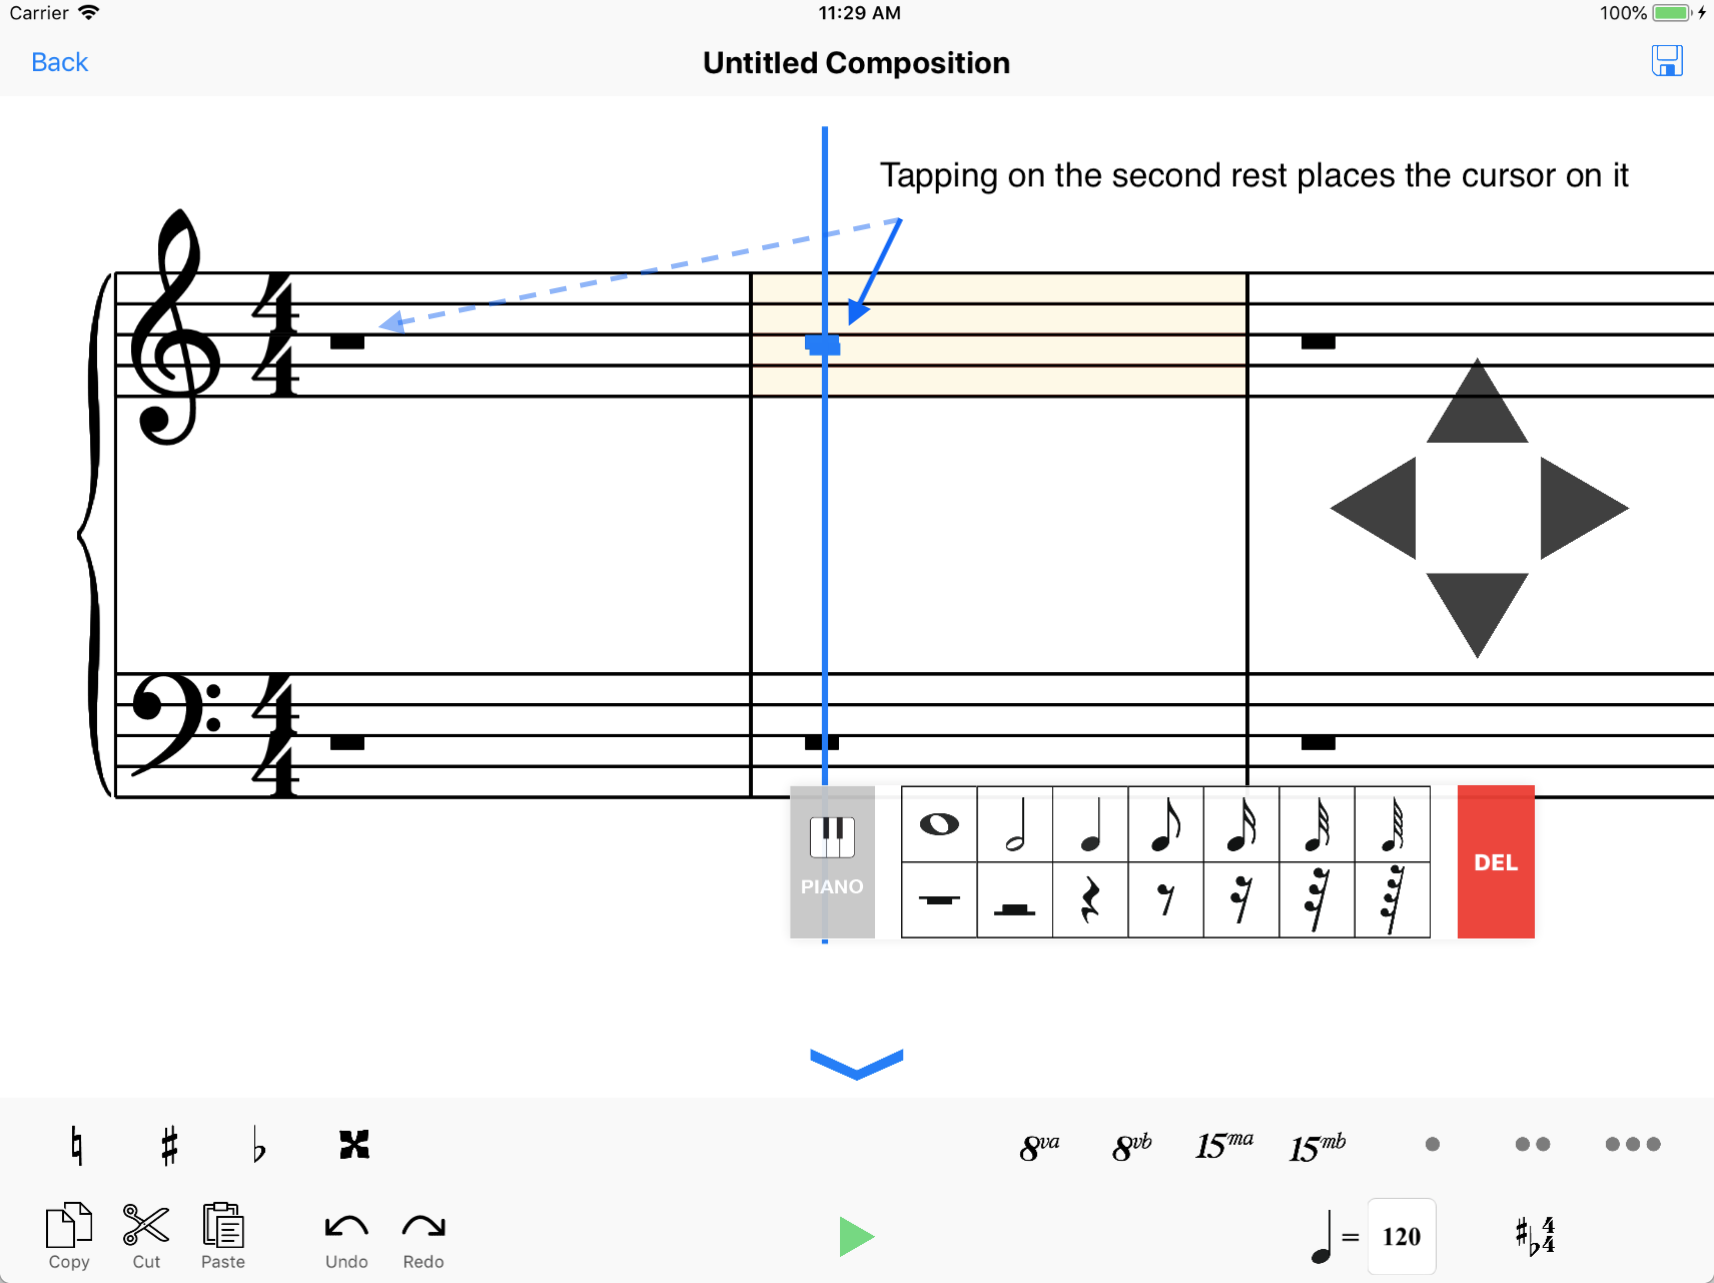
\includegraphics[scale=0.4]{Tap_Cursor}
    \caption{Tap on a location on the editor to move the cursor to it.}
    \label{fig:cursor-tap}
\end{figure}

\subsubsection{Selecting Notes}
A blue highlight on a note or rest indicates that it is currently selected. When a cursor is in the same x-axis with a single note or rest, that note or rest is selected and the user may perform different actions on it such as transpose, edit, or delete (Figure \ref{fig:selected-rest}).

\begin{figure}[H]
	\centering
	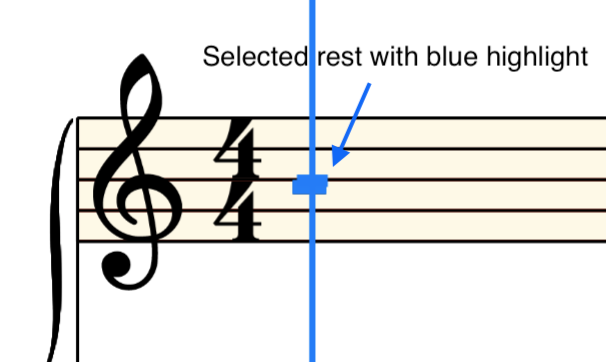
\includegraphics[scale=0.8]{Selected_Rest}
    \caption{Selected rest with blue highlight.}
    \label{fig:selected-rest}
\end{figure}

For selecting multiples notes or rests, the user must do a 1 finger drag gesture in a diagonal direction to bring out the rectangle selector which indicates the area it is currently selecting (Figure \ref{fig:drag-selection}).

\begin{figure}[H]
	\centering
	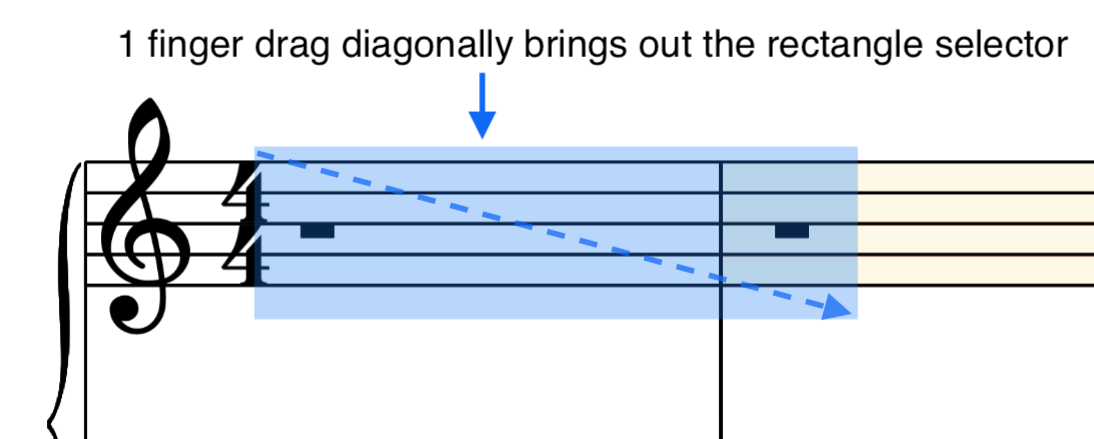
\includegraphics[scale=0.7]{Drag_Selection}
    \caption{1 finger drag diagonally brings out the rectangle selector.}
    \label{fig:drag-selection}
\end{figure}

When the user releases the drag gesture, the rectangle will select the notes it encompassed. Additionally, when more than one rest or note is selected using the drag gesture, it will bring out the transform view which allows the user to transpose, retrograde-inverse, and place a tie or a slur on the selected notes or rests if the rules apply. In the case of Figure \ref{fig:multiple-selected}, the retrograde-inverse and tie or slur buttons are disabled.

\begin{figure}[H]
	\centering
	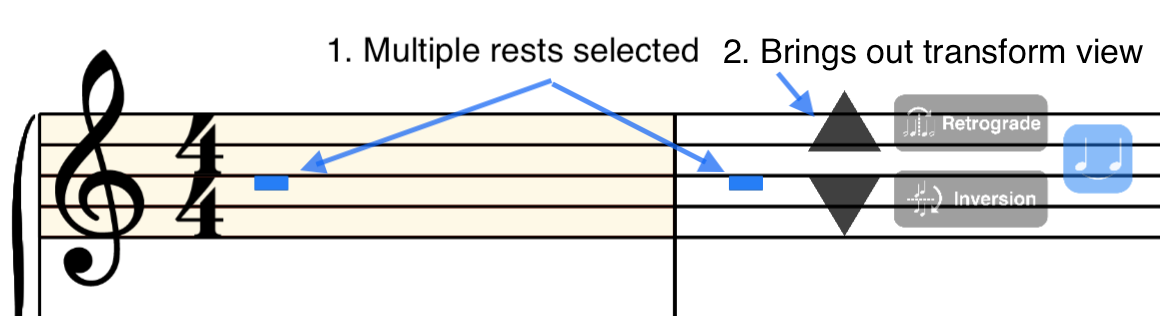
\includegraphics[scale=0.7]{Multiple_Selected}
    \caption{Multiple rests selected with blue highlight and brings out transform view.}
    \label{fig:multiple-selected}
\end{figure}

\subsubsection{Adding a Note or Rest}
Initially, upon creating or opening a composition, the blue cursor automatically selects the first note or rest in the first measure of the composition (Figure \ref{fig:editor}). To add a note or a rest, simply tap on a note type in the notation controls in the editor screen and the note will automatically be added on the location of the blue cursor (Figure \ref{fig:add-note-rest}).

\begin{figure}[H]
	\centering
	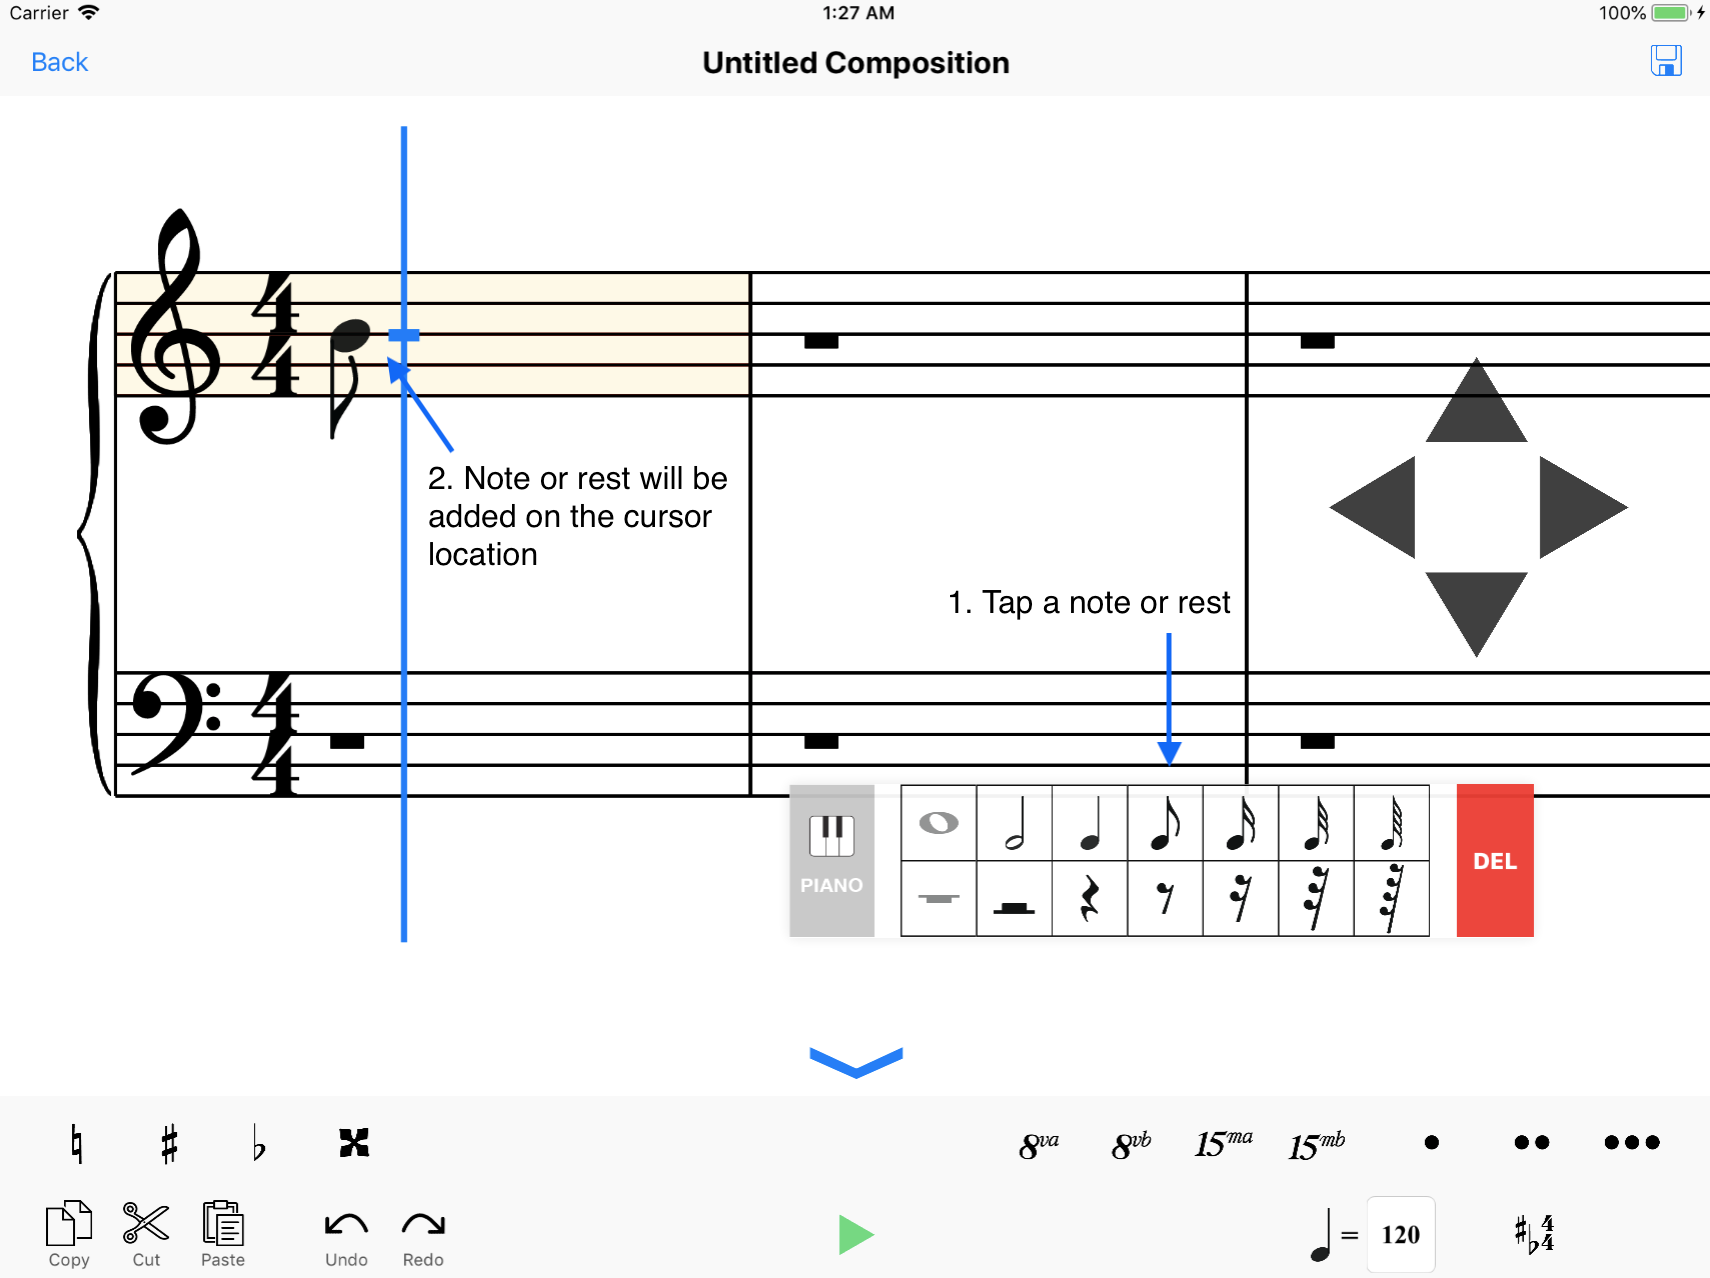
\includegraphics[scale=0.5]{Add_Note_or_Rest}
    \caption{Adding a note or rest.}
    \label{fig:add-note-rest}
\end{figure}

\subsubsection{Adding Polyphony}
To add polyphony, the user must place the cursor above or below an existing note and add a note using the same note type with the existing note.

\begin{figure}[H]
	\centering
	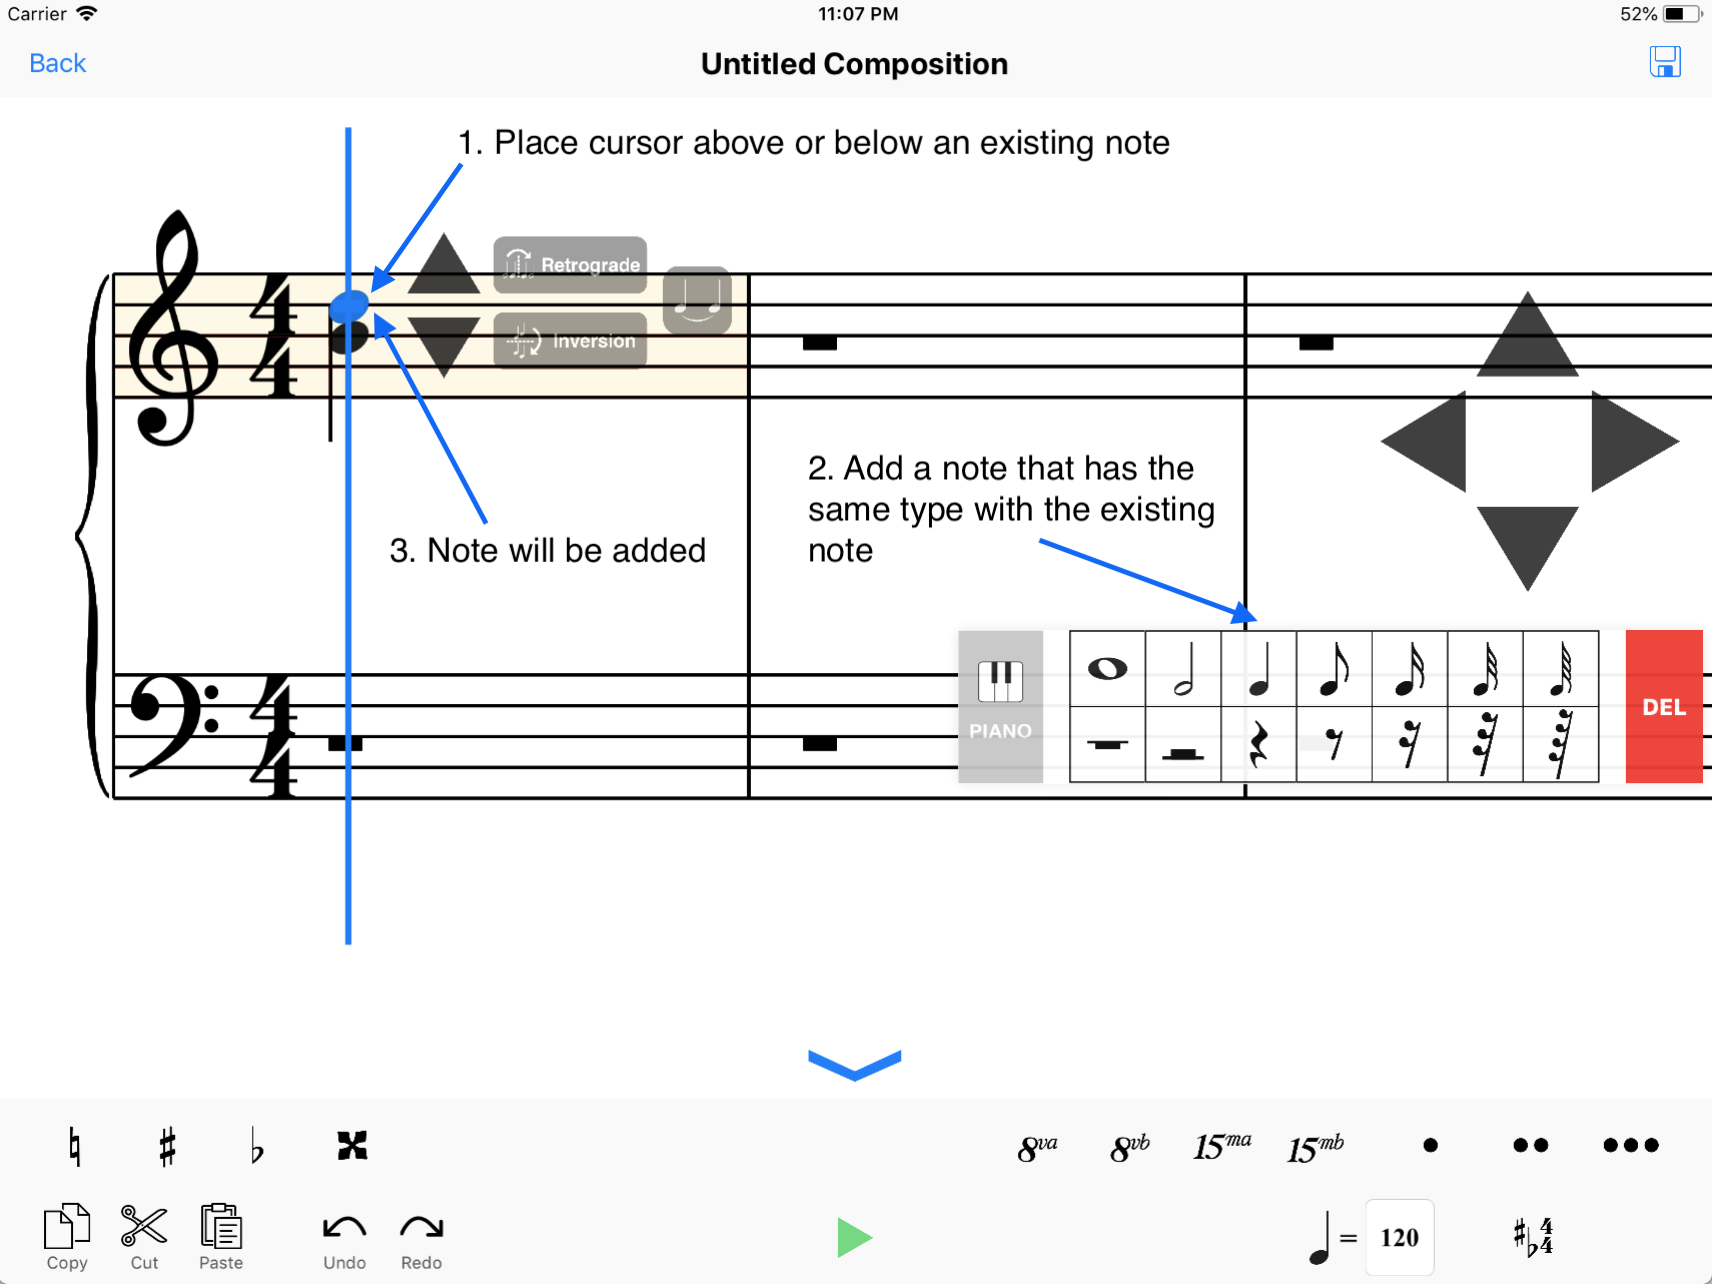
\includegraphics[scale=0.5]{Polyphonic}
    \caption{Adding polyphony.}
    \label{fig:polyphony}
\end{figure}

\subsubsection{Editing Notes}
To edit a note or a group of notes, the user must select the notes that needs editing and tap on the new note type in the notation controls to change the selected notes (Figure \ref{fig:edit-note}).

\begin{figure}[H]
	\centering
	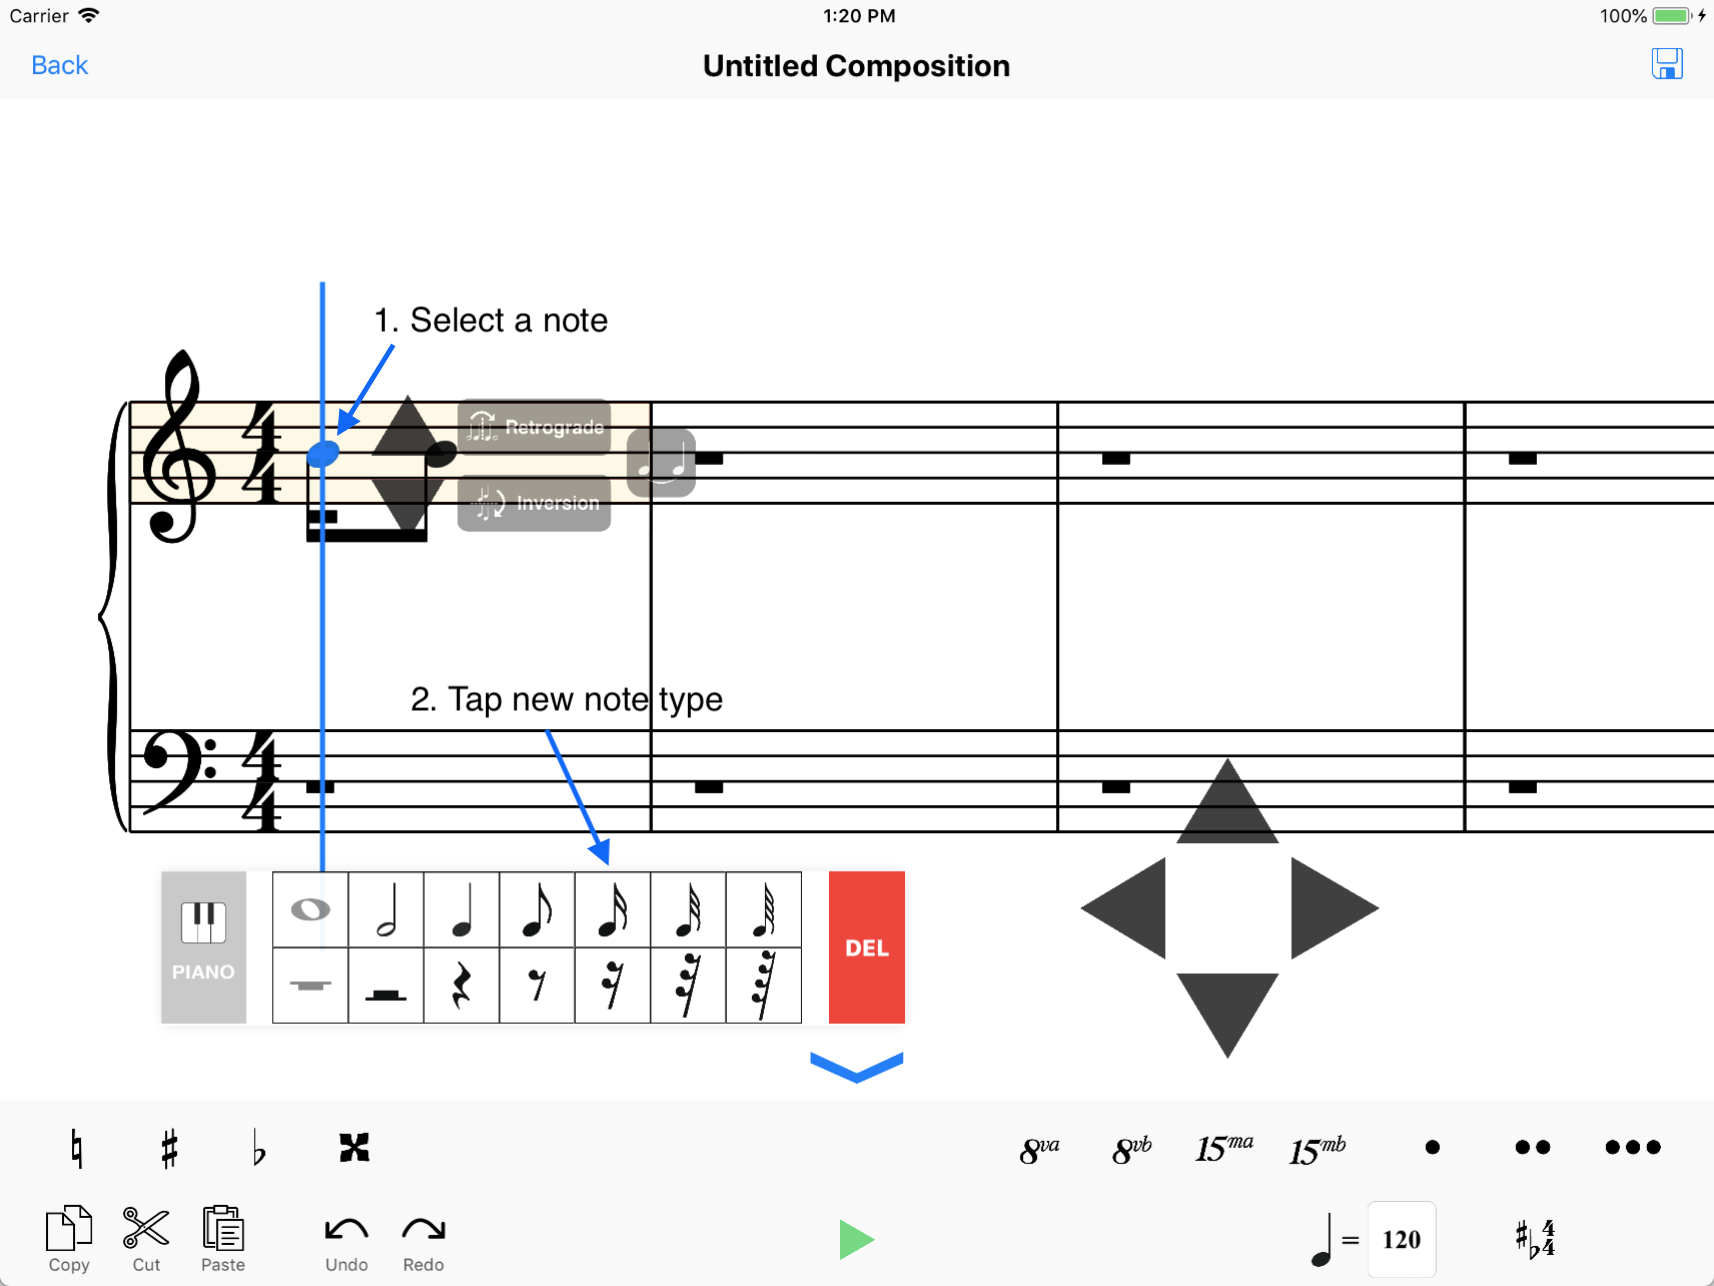
\includegraphics[scale=0.5]{Edit_Note}
    \caption{Editing notes.}
    \label{fig:edit-note}
\end{figure}

\subsubsection{Deleting Notes}
To delete a note or a group of notes, the user must select the notes that needs to be deleted and tap on the delete button in the notation controls to delete the selected notes (Figure \ref{fig:delete-notes}).

\begin{figure}[H]
	\centering
	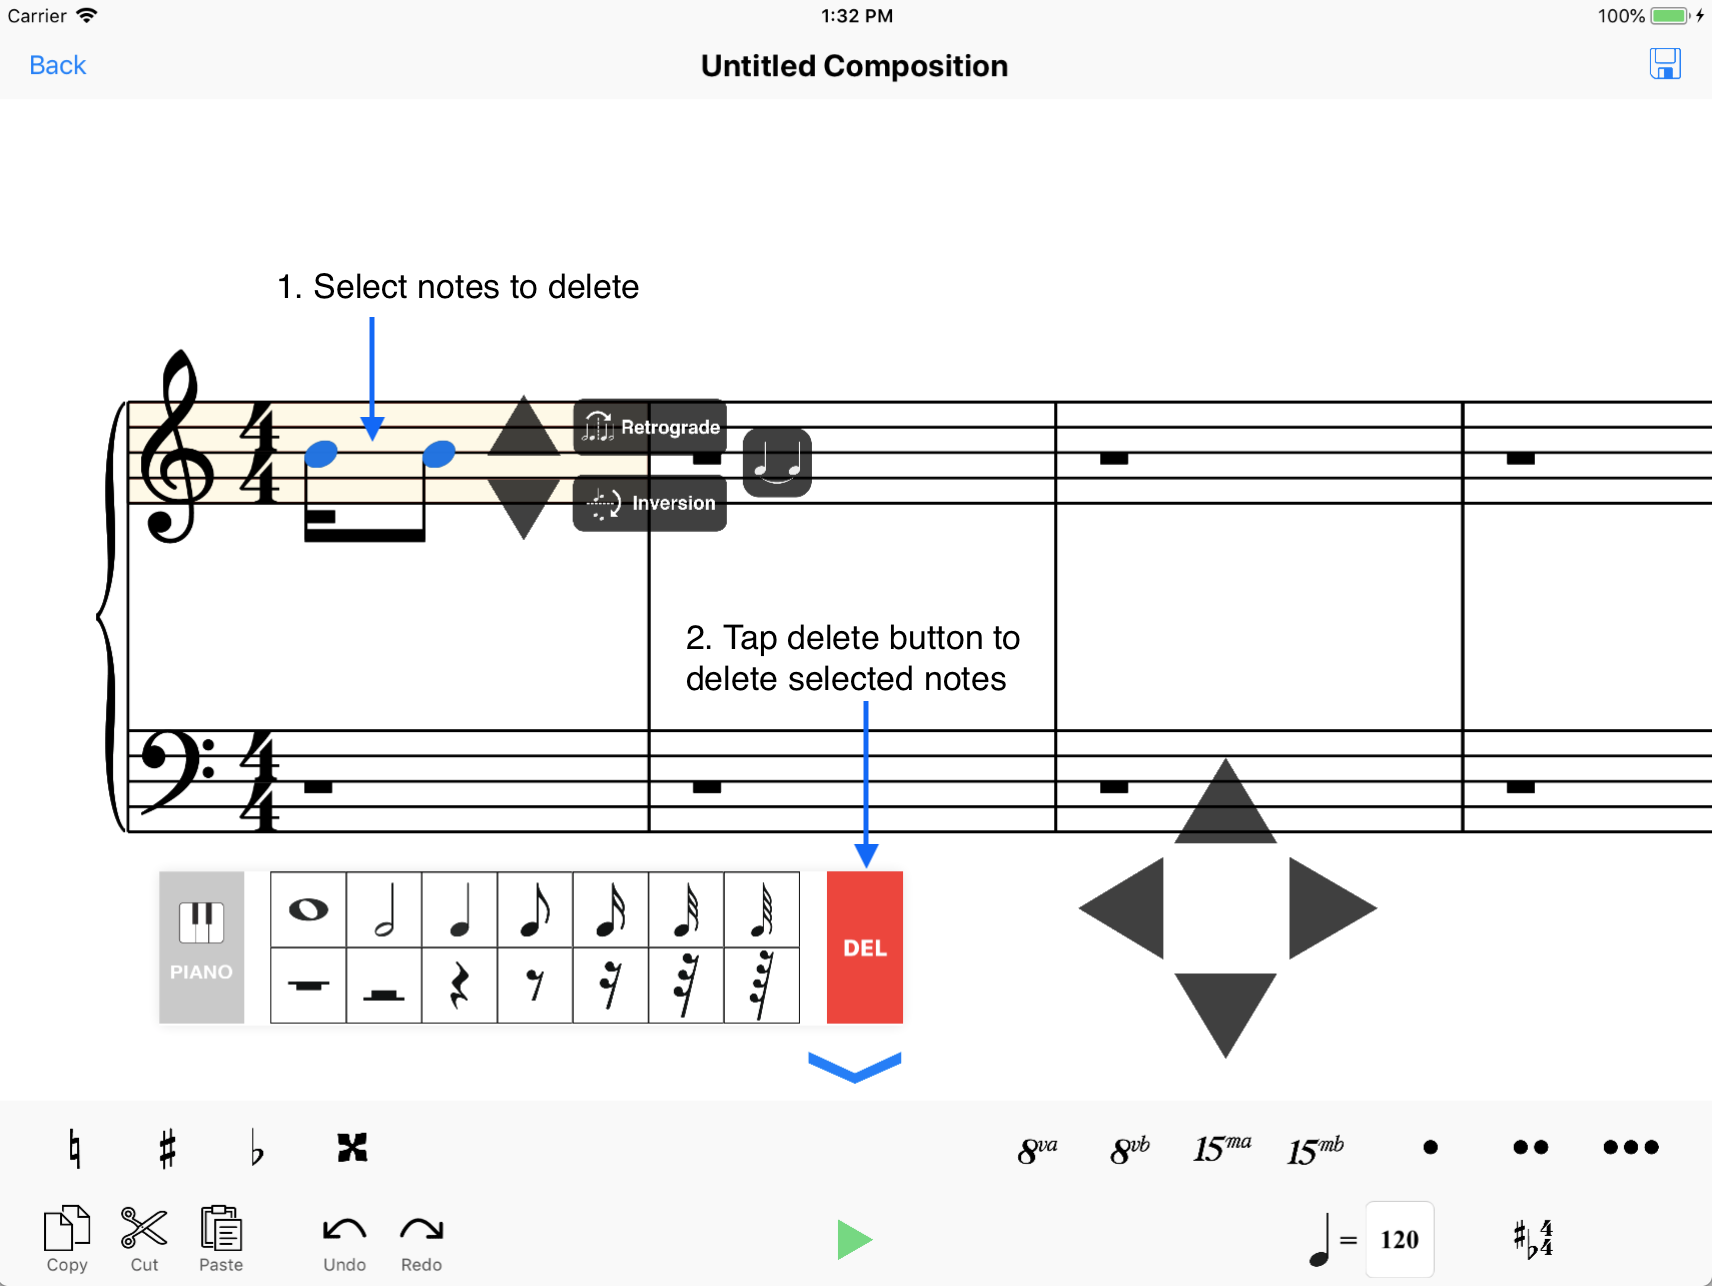
\includegraphics[scale=0.5]{Delete_Notes}
    \caption{Deleting notes.}
    \label{fig:delete-notes}
\end{figure}

\subsubsection{Transposing a Note or a Group of Notes}
To transpose a note or a group of notes, the user must select the notes that needs to be transposed to show the transpose buttons. Upon selecting the notes, the user may tap on the up or down arrow keys beside the selected notes to transpose them half step higher or lower, respectively (Figure \ref{fig:transposing}).

\begin{figure}[H]
	\centering
	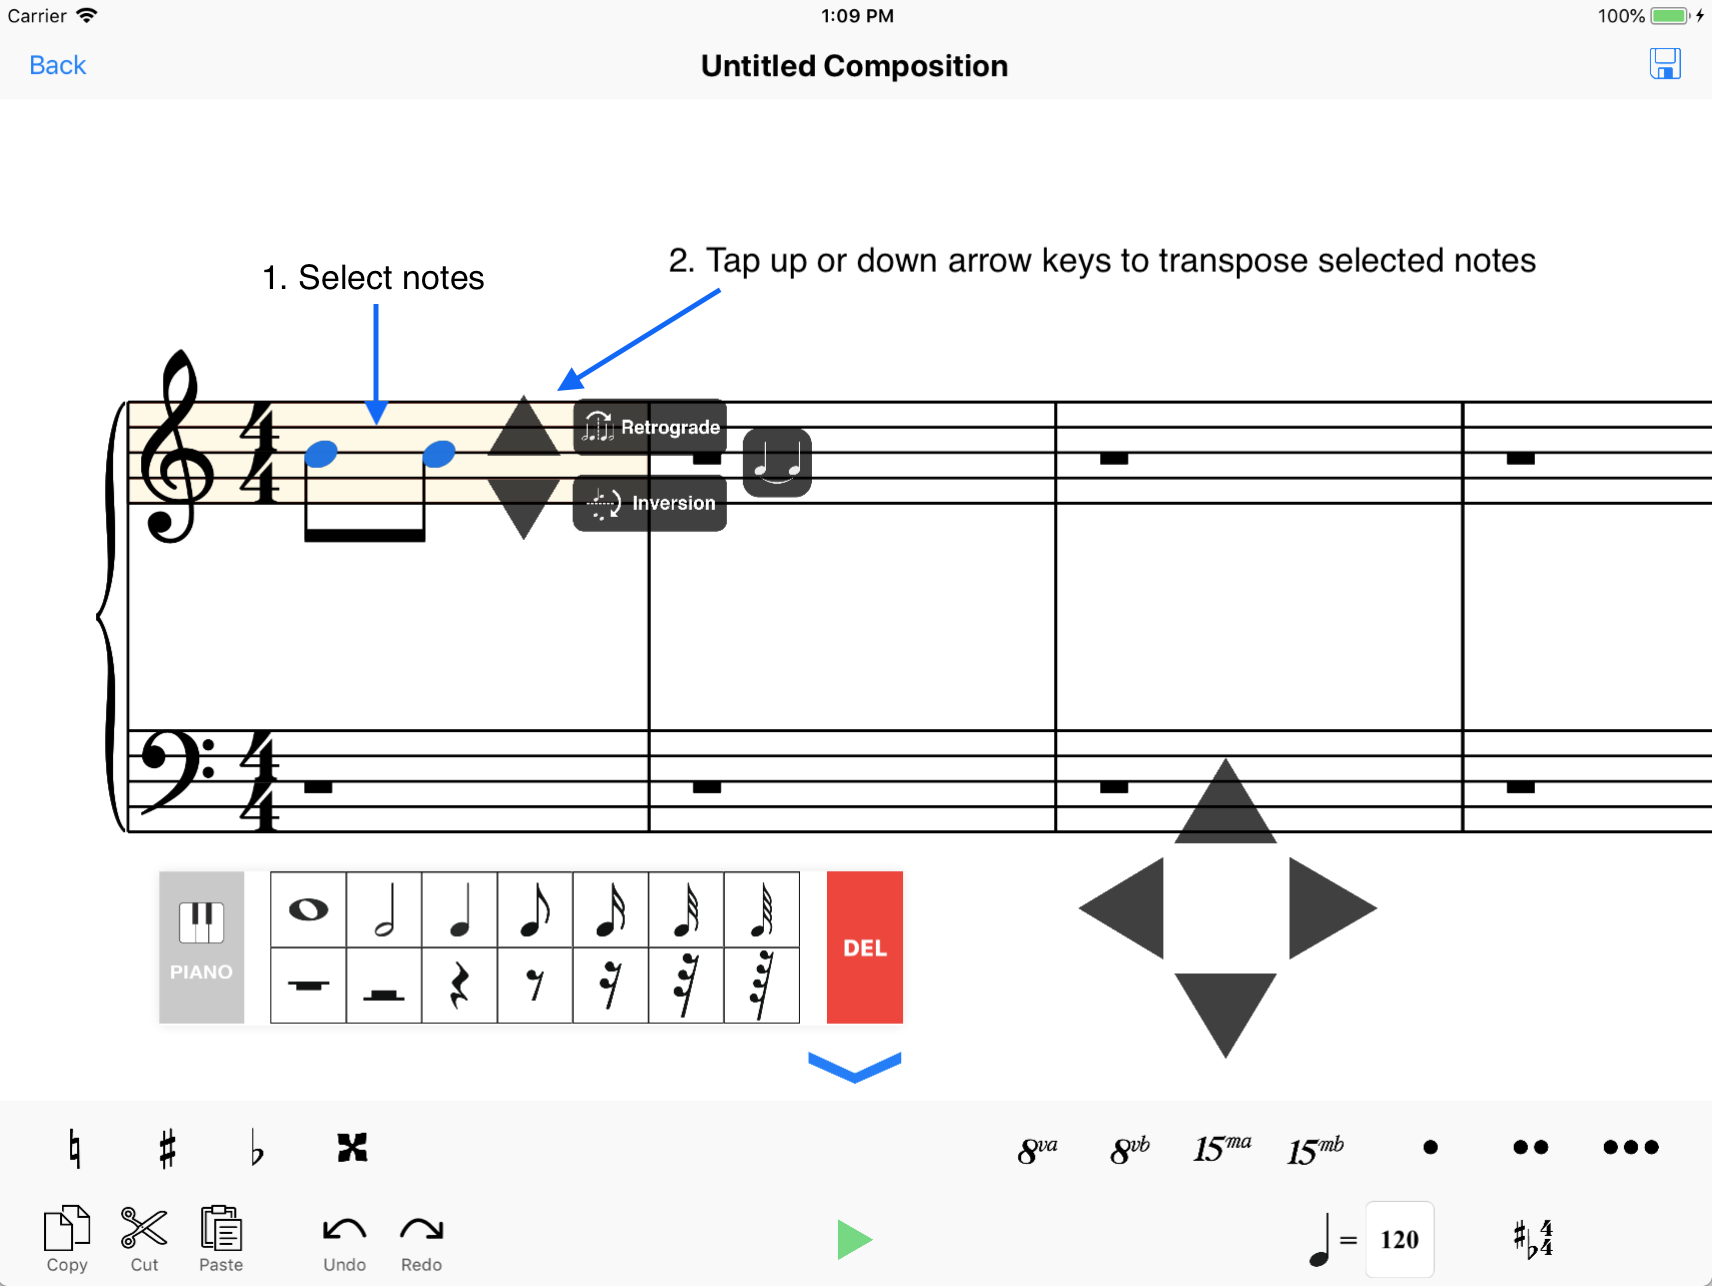
\includegraphics[scale=0.5]{Transposing}
    \caption{Transposing notes.}
    \label{fig:transposing}
\end{figure}

\subsubsection{Retrograde - Inversion}
Retrograde - inversion can be performed only if there are more than one note selected. The transform view beside the selected notes will appear upon selecting notes and the retrograde and inverse buttons will be enabled allowing the user to tap either of them (Figure \ref{fig:r-i}).

\begin{figure}[H]
	\centering
	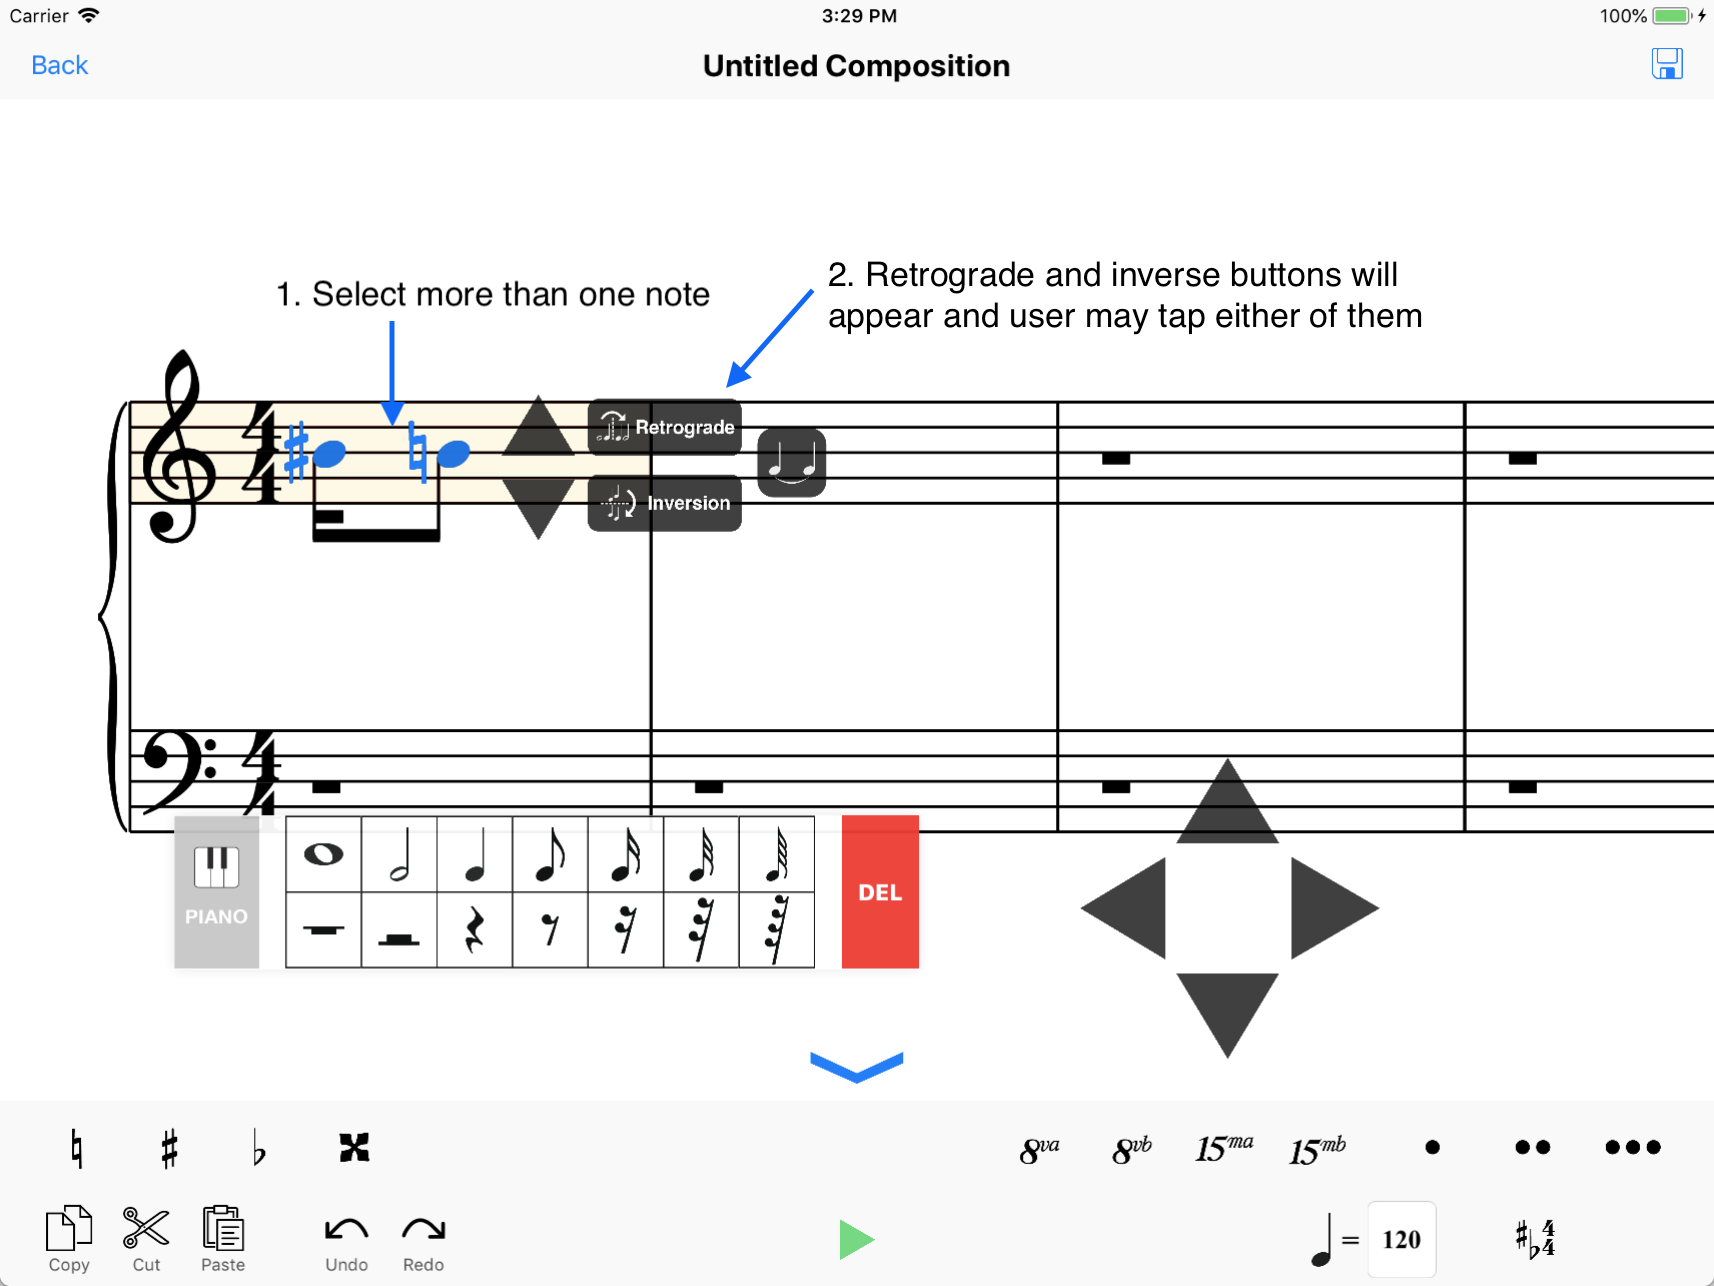
\includegraphics[scale=0.5]{Retrograde_Inverse}
    \caption{Performing a retrograde or inversion on a group of notes.}
    \label{fig:r-i}
\end{figure}

\subsubsection{Adding Ties or Slurs}
Ties or slurs could be added by selecting more than one note. The transform view beside the selected notes will appear and the tie or slur button will be enabled allowing the user to add a tie or slur on the selected notes. A tie will will be added if the selected notes are all the same pitch, on the other hand, a slur will be added if at least one of the selected notes has a different pitch. Additionally, if a user transposes a note that has a tie or a slur, it automatically changes the type depending whether the connection of all the notes have the same pitch or not (Figure \ref{fig:ties-slur}).

\begin{figure}[H]
	\centering
	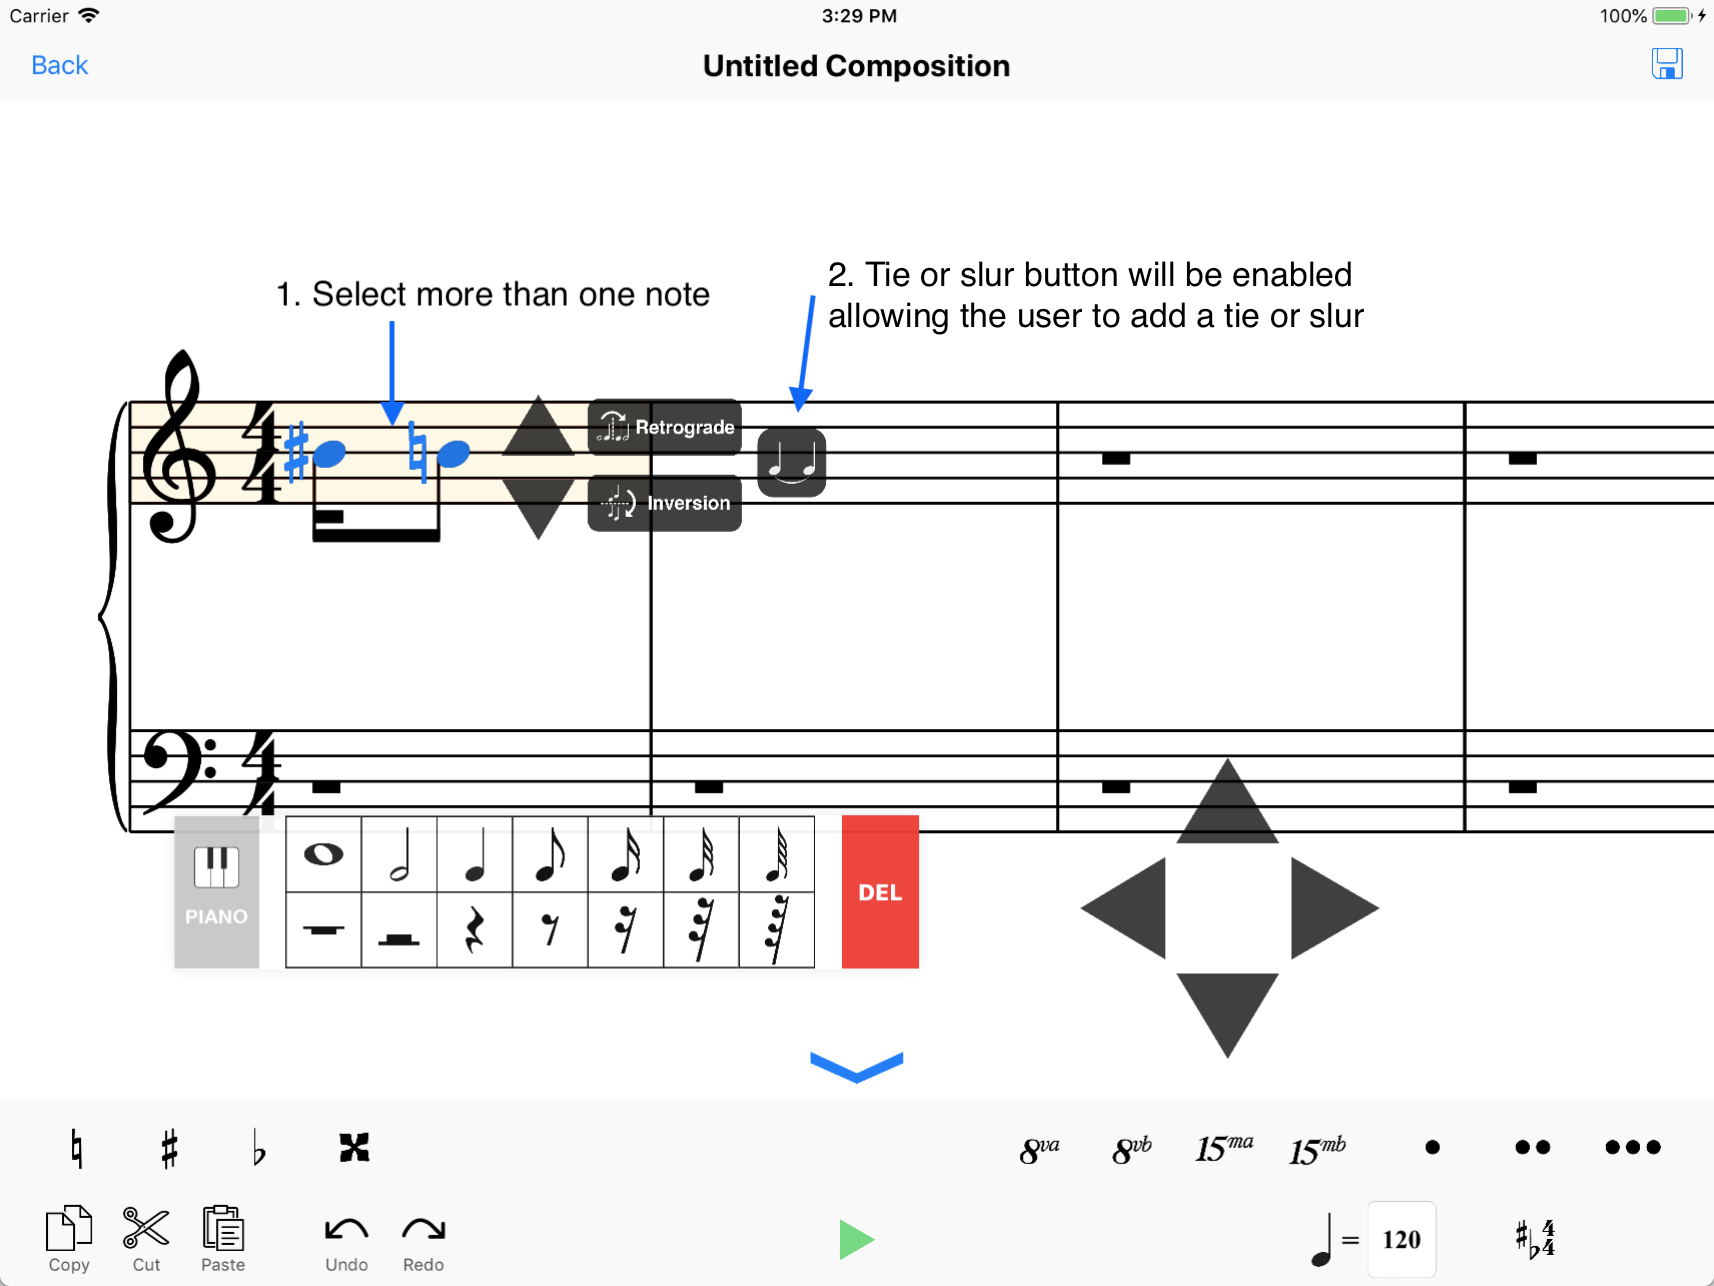
\includegraphics[scale=0.5]{Tie_Slur}
    \caption{Adding ties or slurs.}
    \label{fig:ties-slur}
\end{figure}

\subsubsection{Adding and Removing Note Accidentals, Ottava, and Dots}
The accidental buttons are located in the bottom menu of the editor. The behavior of adding and removing accidentals are similar on how the toggling of font types in word processors work. To explain further, an example would be two selected notes that initially do not have any accidentals. After tapping an accidental from the bottom menu with the two notes selected, it would change the type of accidental of all the notes selected. Selected notes with the same accidentals would highlight the accidental button with blue in the bottom menu to show that it could be toggled or tapped again to remove the accidentals in all the notes that are selected (Figure \ref{fig:add-accidental-notes}). In this example, the sharp icon is only added on the first note because the selected notes have the same pitch and the same accidental, but both notes really have a sharp accidental. This is so because of the rules of music notation.

\begin{figure}[H]
	\centering
	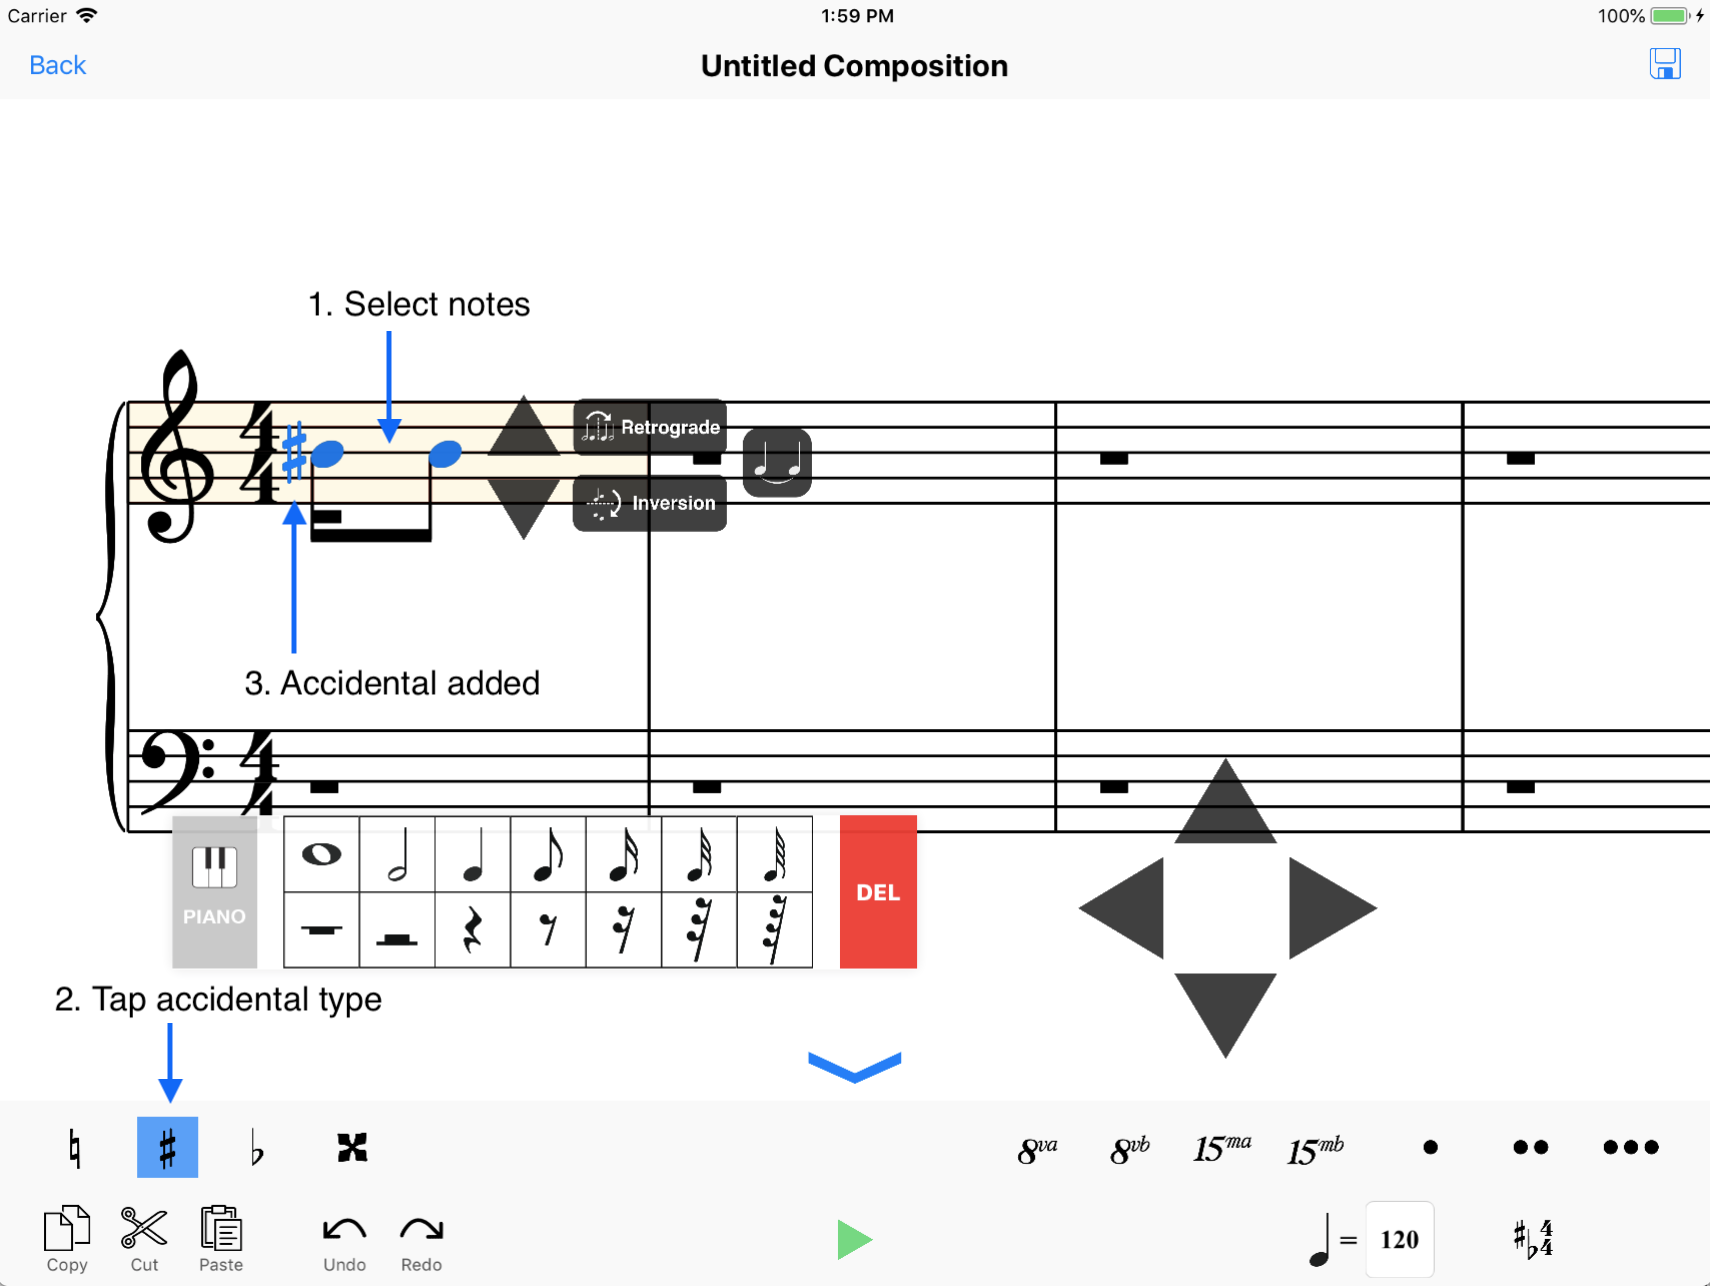
\includegraphics[scale=0.5]{Add_Accidental_Notes}
    \caption{Adding accidental on multiple notes.}
    \label{fig:add-accidental-notes}
\end{figure}

Another case would be when a note has a sharp and another note does not have an accidental. When both notes are selected, and the user taps on any accidental, it will change all the selected notes to the tapped accidental (Figure \ref{fig:change-accidental-notes}).

\begin{figure}[H]
	\centering
	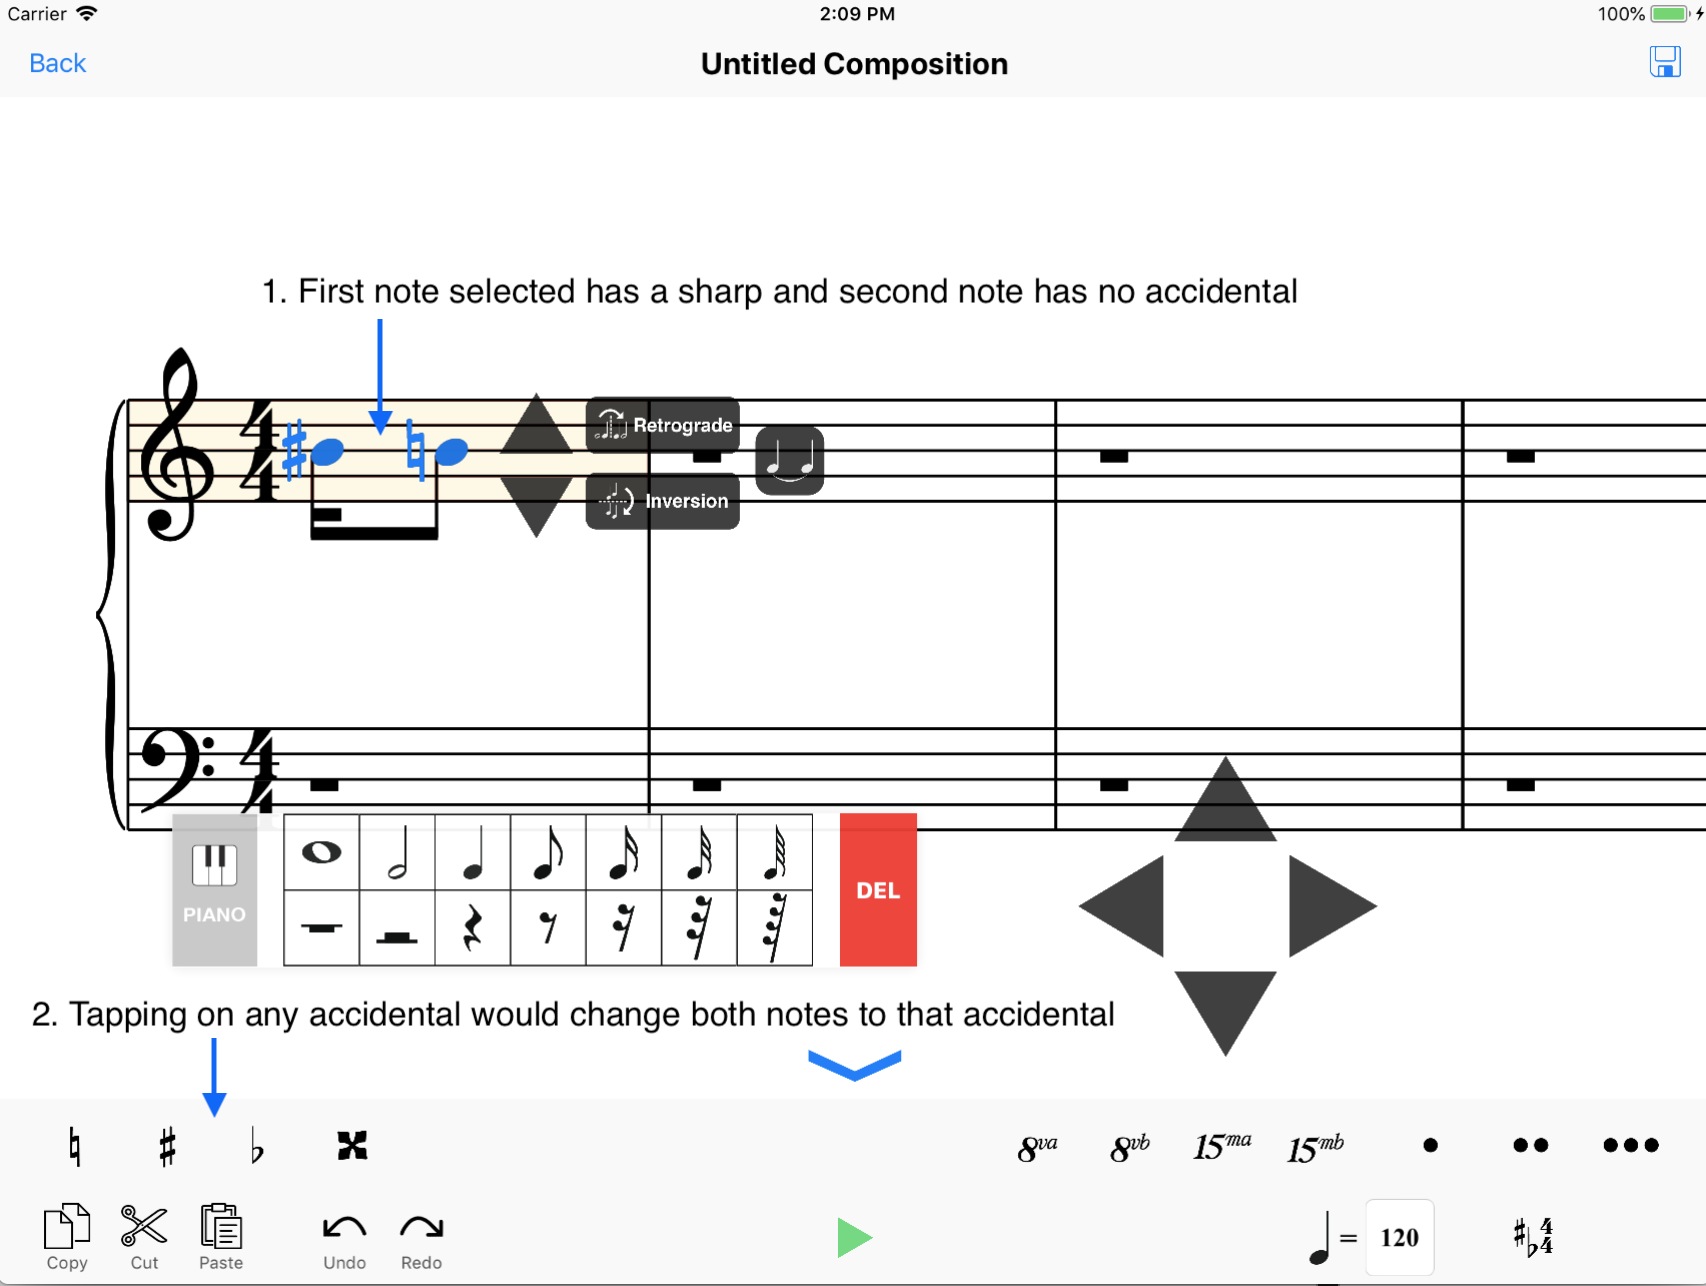
\includegraphics[scale=0.5]{Change_Accidental_Notes}
    \caption{Changing accidental on multiple notes with different accidentals.}
    \label{fig:change-accidental-notes}
\end{figure}

Removing accidentals, on the other hand, works by selecting a note with an accidental and tapping the same accidental again. When a single note with accidental is selected, the corresponding accidental button type would highlight blue in the bottom menu and the user may tap it to remove the accidental on the selected note (Figure \ref{fig:remove-note-accidental}).

\begin{figure}[H]
	\centering
	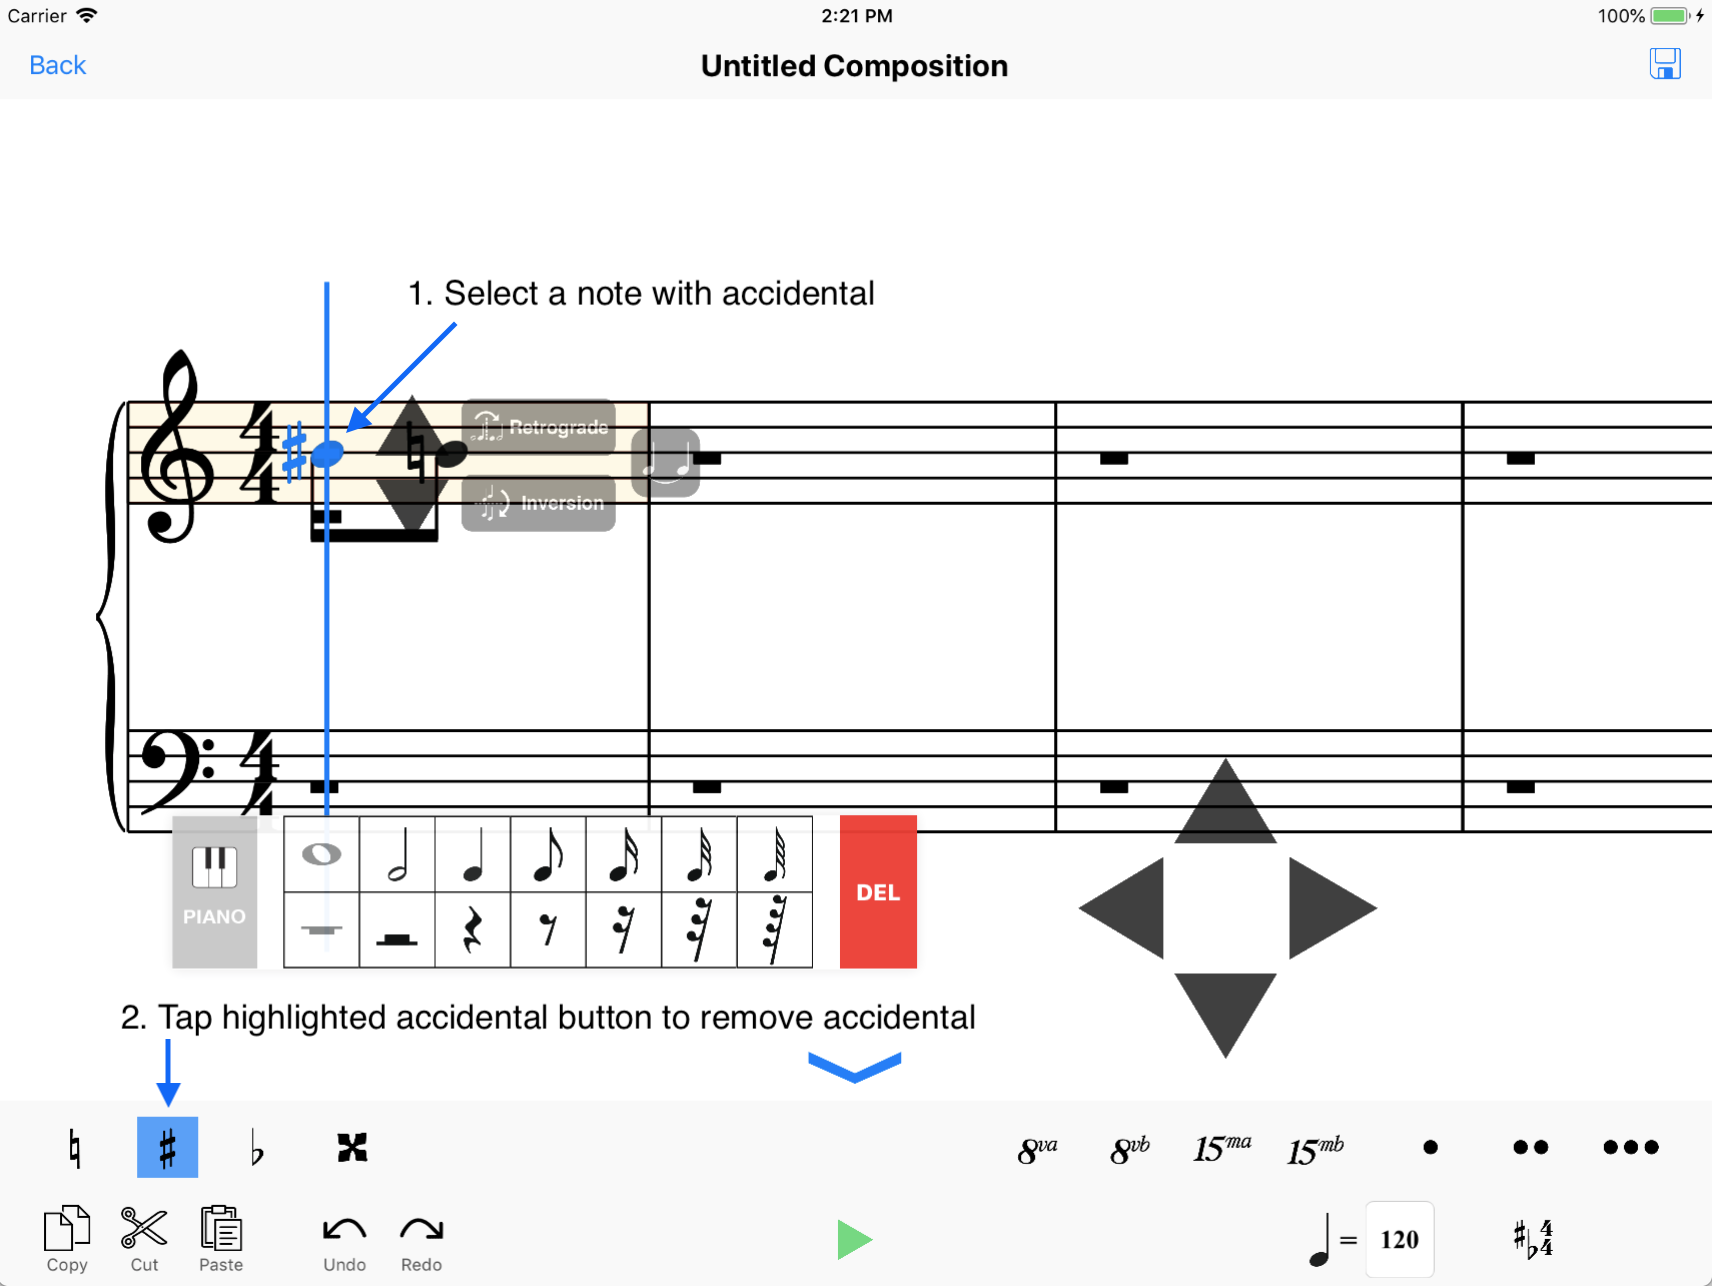
\includegraphics[scale=0.5]{Remove_Note_Accidental}
    \caption{Removing a note accidental.}
    \label{fig:remove-note-accidental}
\end{figure}

There is an alternative way of placing accidentals. This is done by tapping on any accidental button where there is no selected note. When an accidental button is highlighted and no note is selected, all notes that are added will automatically have the accidental selected. To unselect an accidental type, simply place the cursor where there is no note or rest again and tap the highlighted accidental button (Figure \ref{fig:alt-accidental}).

\begin{figure}[H]
	\centering
	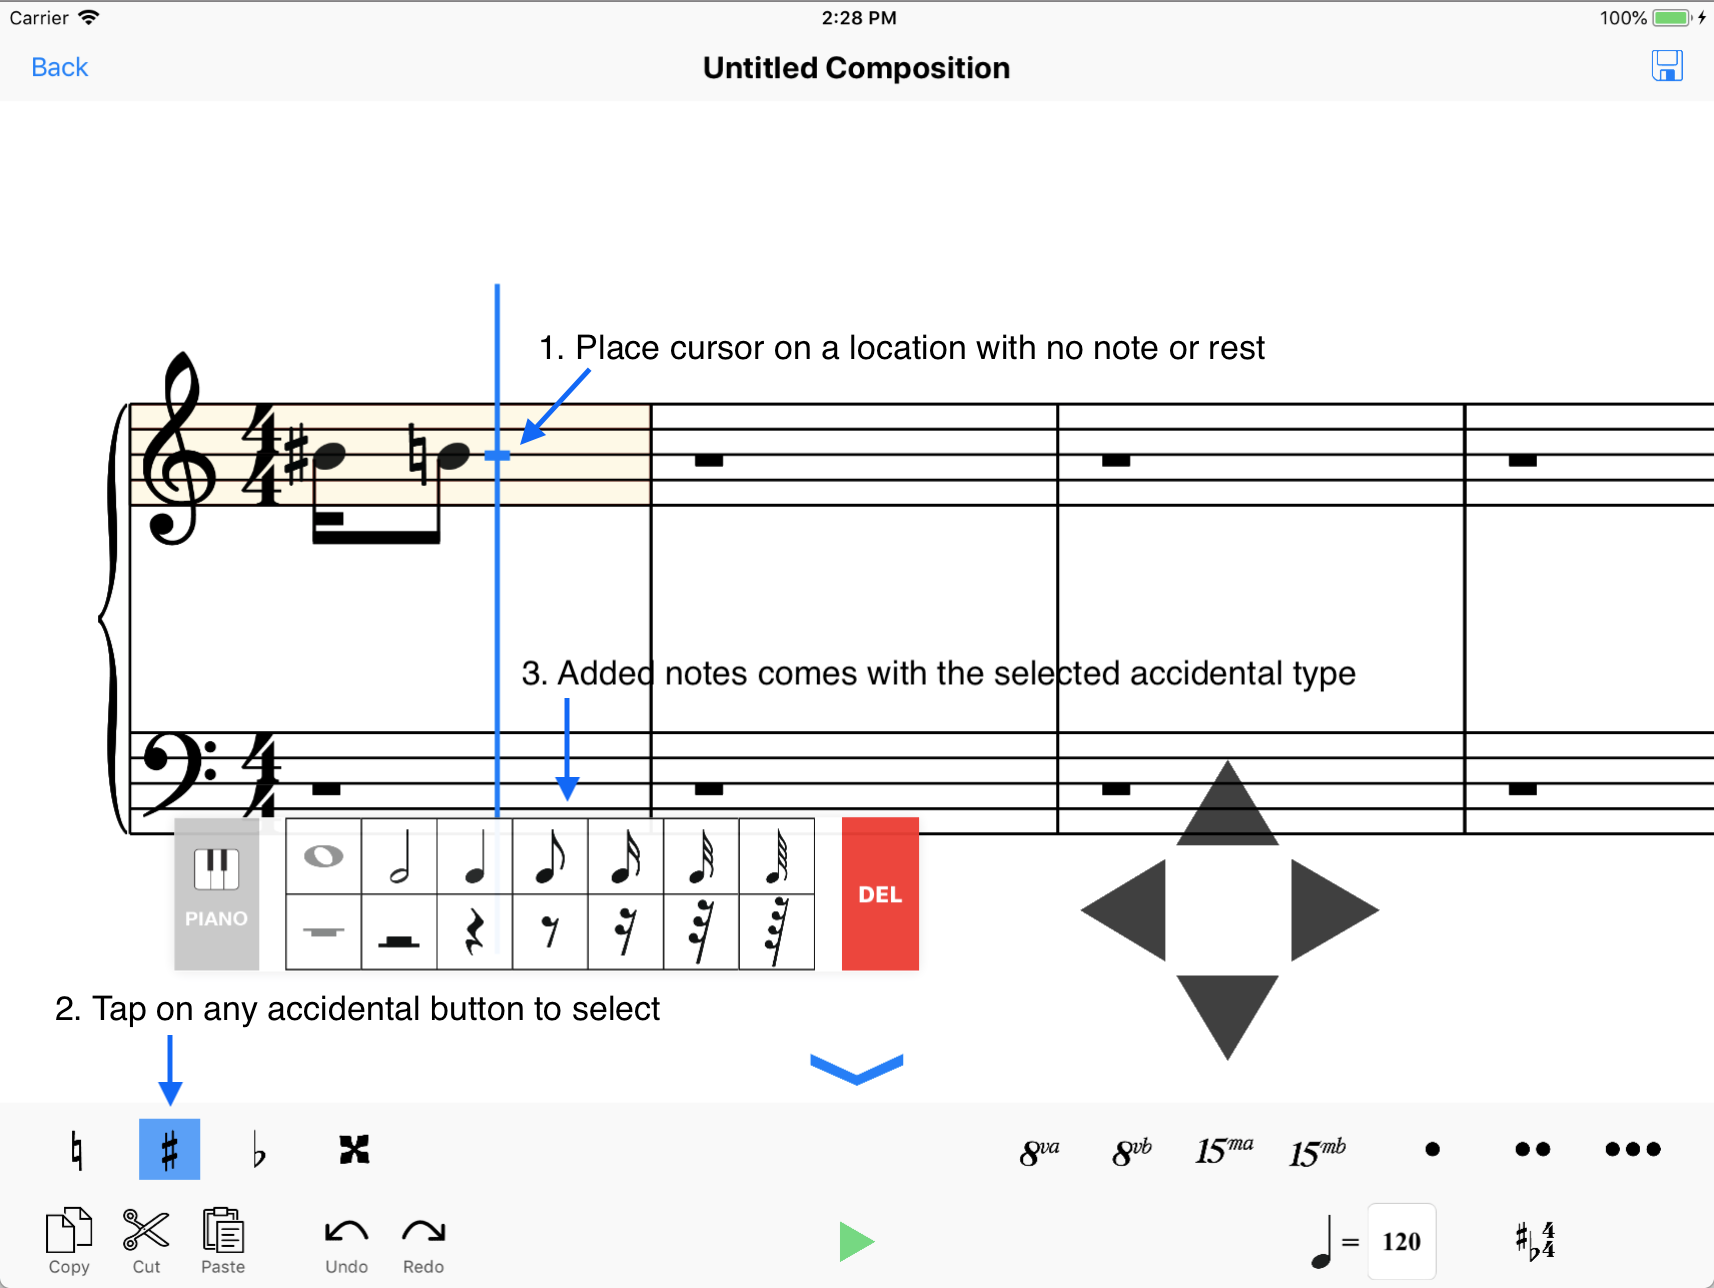
\includegraphics[scale=0.5]{Alt_Accidental}
    \caption{Alternative accidental input.}
    \label{fig:alt-accidental}
\end{figure}

The same behavior is implemented for adding and removing ottava and dots.

\subsubsection{Copying, Cutting, and Pasting Notes or Rests}
To copy or cut notes, the user must select the notes first and then tap on the copy or cut button in the bottom menu. After copying or cutting the notes, the user may then tap on the paste button to paste the notes on the location of the cursor (Figure \ref{fig:copy-cut-paste}).

\begin{figure}[H]
	\centering
	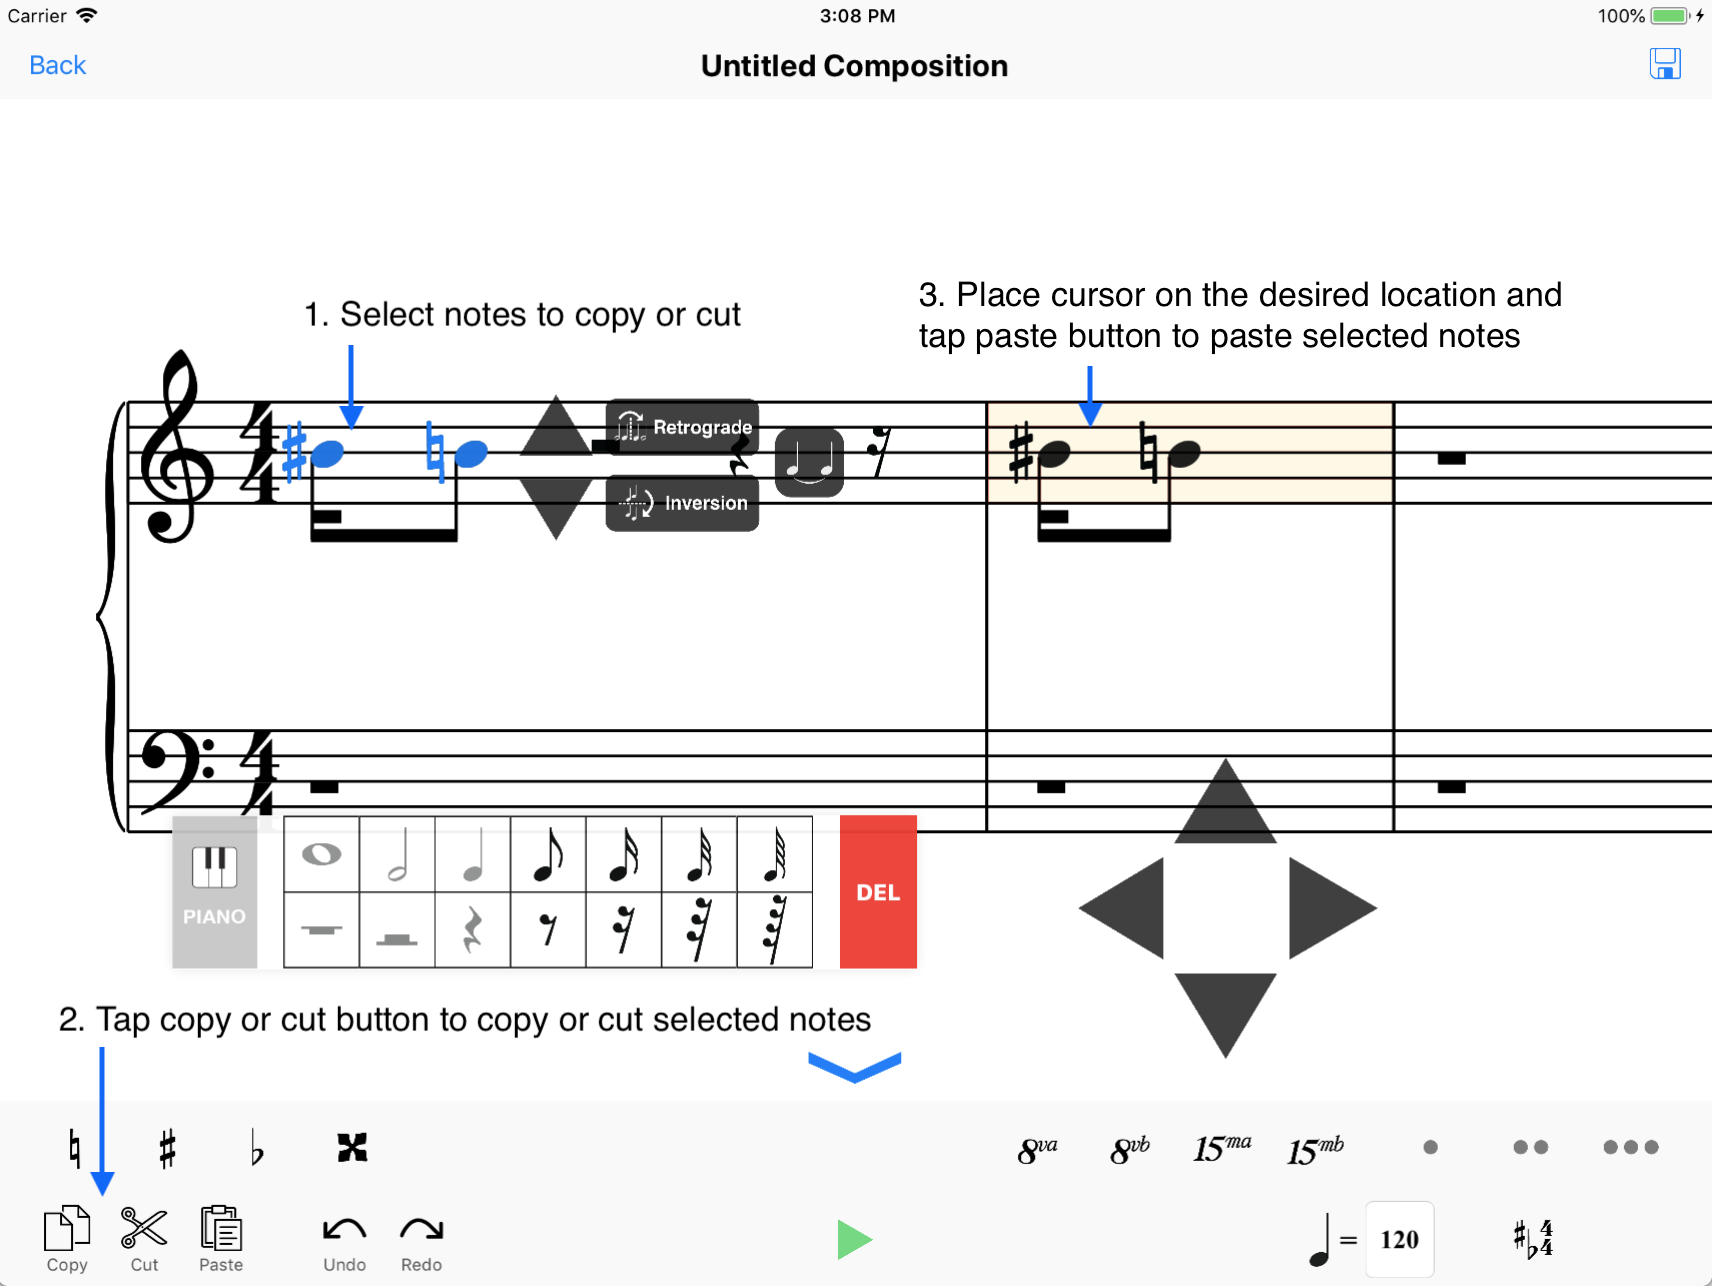
\includegraphics[scale=0.5]{Copy__Cut__Paste}
    \caption{Copying, cutting, and pasting notes.}
    \label{fig:copy-cut-paste}
\end{figure}

\subsubsection{Undoing and Redoing Actions}
To undo or redo an action, the user must tap on the undo or redo button in the bottom menu (Figure \ref{fig:undo-redo}).

\begin{figure}[H]
	\centering
	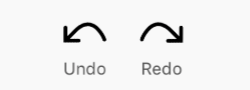
\includegraphics[scale=0.8]{Undo_Redo}
    \caption{Undoing or Redoing actions.}
    \label{fig:undo-redo}
\end{figure}

\subsubsection{Changing the Tempo}
There are two ways of changing the tempo of a composition. The first way is by tapping on the tempo icon in the bottom right part of the menu, and the slider will appear allowing the user to slide it to the left or to the right whilst increasing or decreasing the tempo, respectively (Figure \ref{fig:tempo-slider}). Tapping anywhere outside the tempo slider would hide it.

\begin{figure}[H]
	\centering
	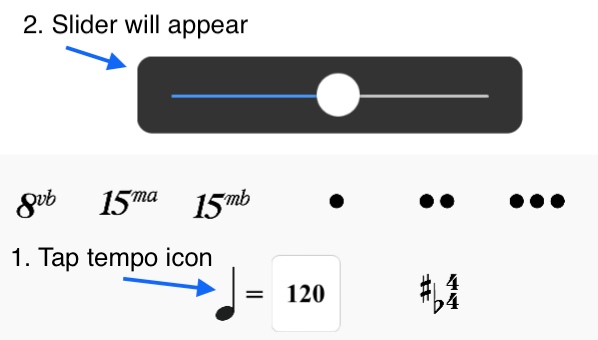
\includegraphics[scale=0.8]{Change_Tempo1}
    \caption{Changing the tempo using a slider.}
    \label{fig:tempo-slider}
\end{figure}

The second way of changing the tempo is by simply tapping on the textbox beside the tempo icon which allows the user to type in the desired tempo (Figure \ref{fig:tempo-type}).

\begin{figure}[H]
	\centering
	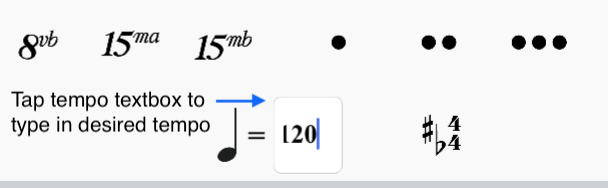
\includegraphics[scale=0.8]{Change_Tempo2}
    \caption{Changing the tempo by typing in the textbox.}
    \label{fig:tempo-type}
\end{figure}

\subsubsection{Changing Time Signature and Key Signature}
To change the time signature and key signature of the composition, the user must tap on the time / key signature button (Figure \ref{fig:tim-sig-btn}) on the bottom right part of the menu.

\begin{figure}[H]
	\centering
	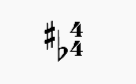
\includegraphics[scale=1]{Time_Sig_Btn}
    \caption{Time / Key Signature Button.}
    \label{fig:tim-sig-btn}
\end{figure}

After tapping the time / key signature button, a menu will appear which lets the user set both the time signature and key signature (Figure \ref{fig:tim-sig-menu}). To edit the time signature, the user may tap on one of the preset buttons which will set the values of the number of beats and beat duration automatically. Alternatively, the user may may manually enter the values for the number of beats and beat duration by tapping on their corresponding textboxes. Upon saving the changes of the new time signature, the notes inside the measures that are affected by the change will automatically readjust their location depending on the newly set time signature. In changing the key signature, the user may tap on one of the circular buttons for the key signature. After saving, changes will also affect the notes inside the affected measures.

\begin{figure}[H]
	\centering
	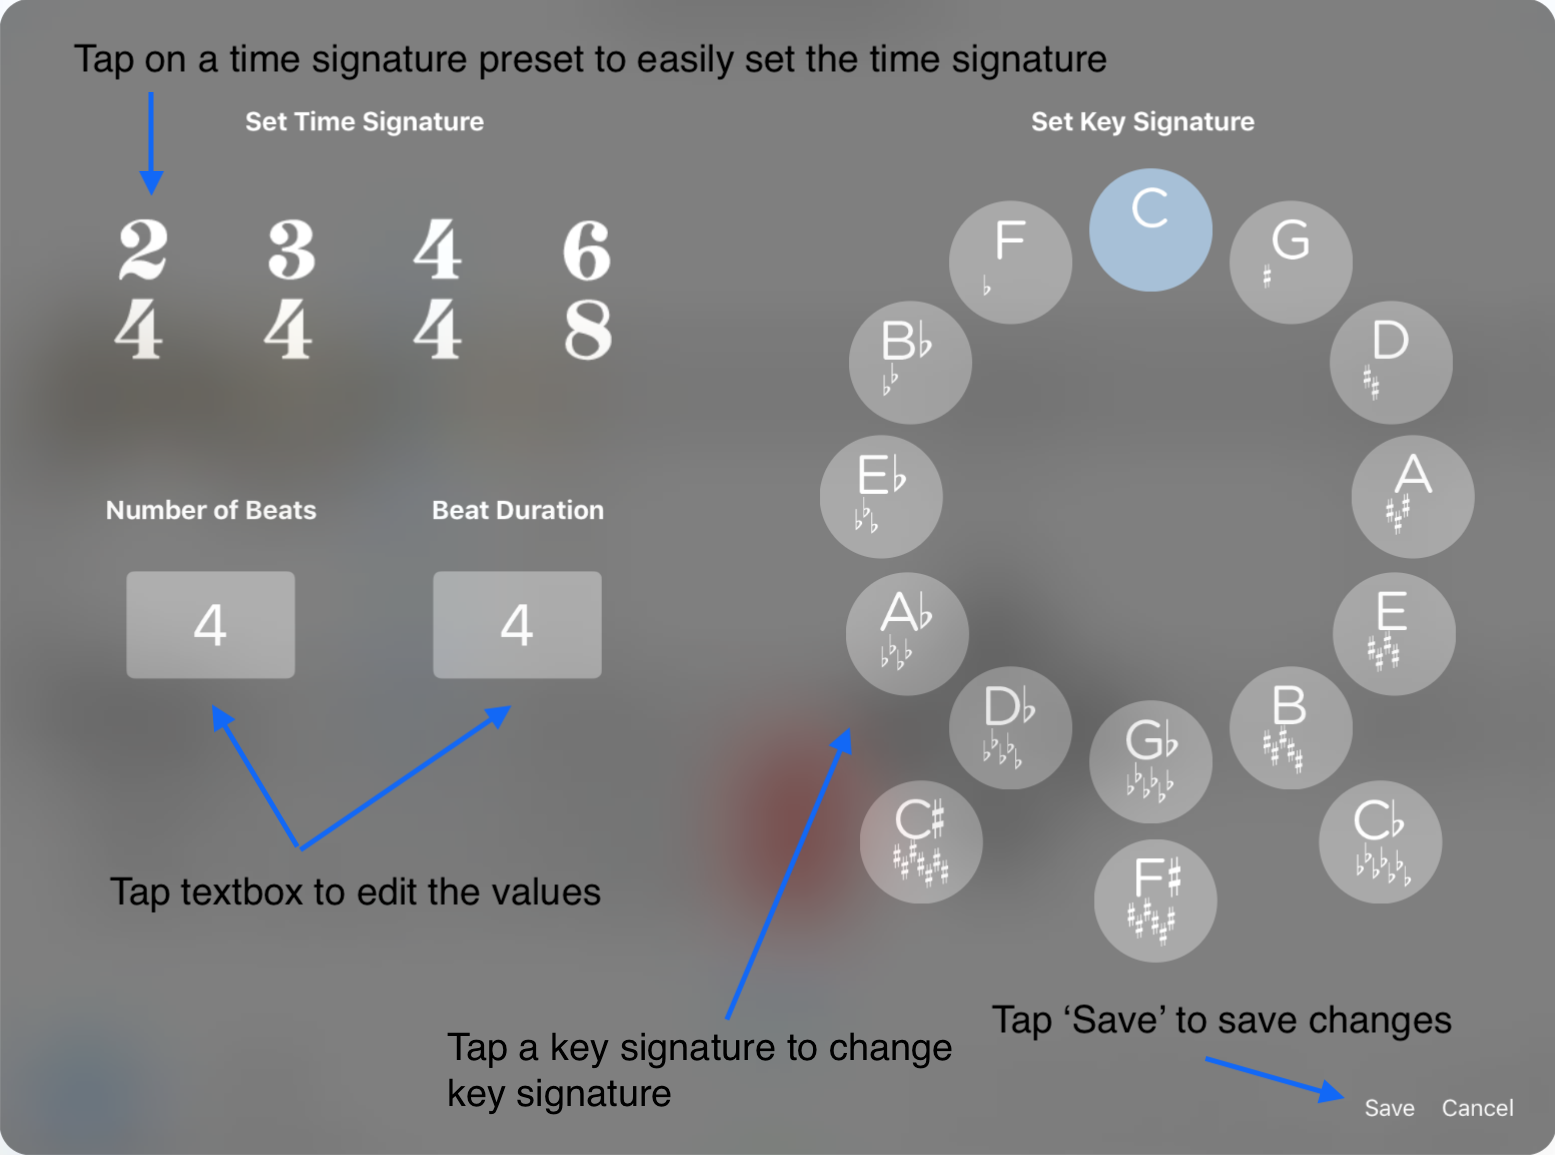
\includegraphics[scale=0.5]{Time_Sig_Menu}
    \caption{Time / Key Signature Menu.}
    \label{fig:tim-sig-menu}
\end{figure}

\subsubsection{Using the Keyboard for Note Input}
The application does not only allow users to add notes through the notation controls, but there is also an alternative way to add notes through the virtual keyboard. To activate the keyboard input, the user must tap on the keyboard button in the left side of the notation controls which brings out the virtual keyboard interface (Figure \ref{fig:keyboard}). After activating the keyboard input, the user may tap on a note type in the notation controls to change the type of note that will be added when pressing a key in the keyboard. Upon pressing a key in the keyboard, the note will be added on the location of the cursor with the corresponding pitch that was pressed on the keyboard and also the selected note type from the notation controls. To deactivate the keyboard input, the user must simply tap on the keyboard button again to hide the keyboard interface and go back to the original method of input.

\begin{figure}[H]
	\centering
	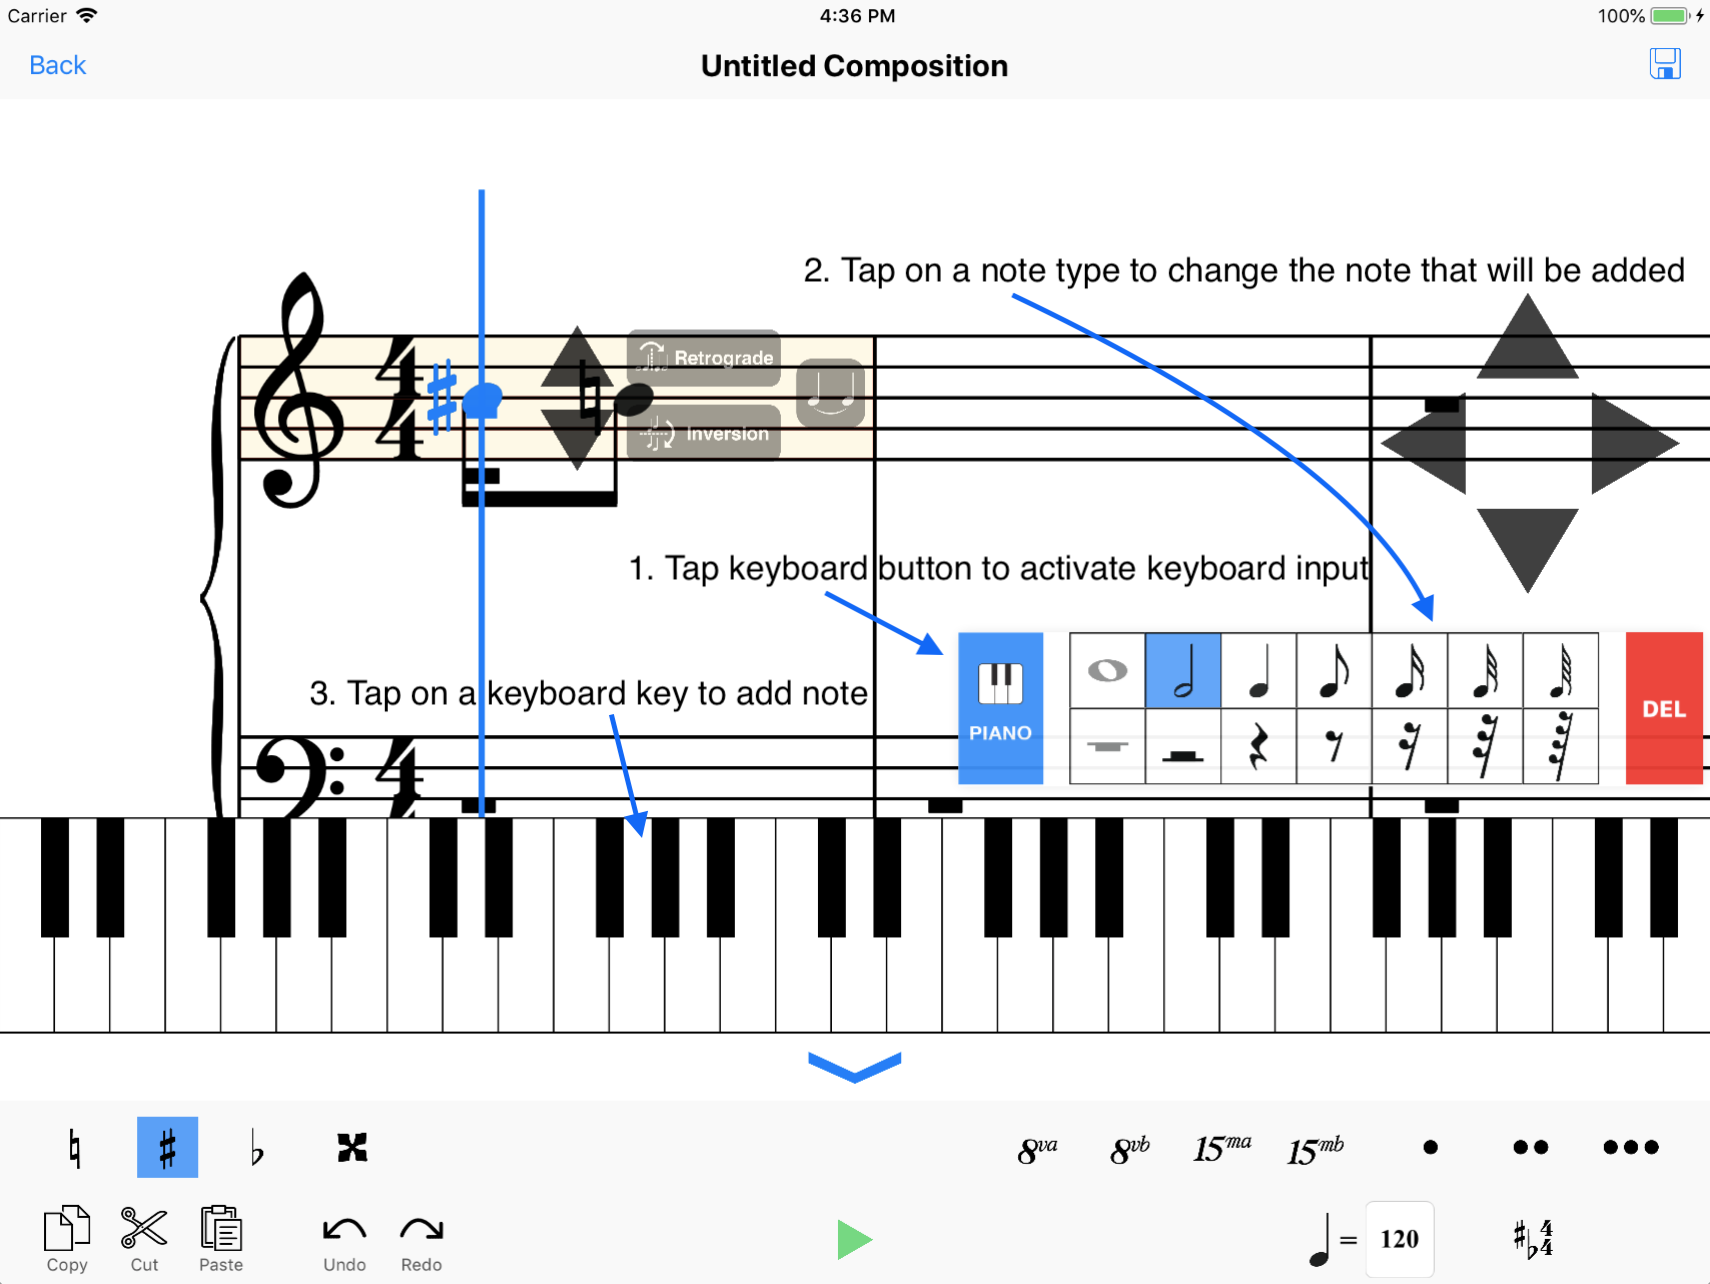
\includegraphics[scale=0.5]{Keyboard}
    \caption{Keyboard input.}
    \label{fig:keyboard}
\end{figure}

\subsubsection{Playing the Composition}
To play the composition, the user must simply tap on the play button on the bottom menu. Playback starts on the currently selected measure and note. The currently selected measure is the measure highlighted with yellow (Figure \ref{fig:play}).

\begin{figure}[H]
	\centering
	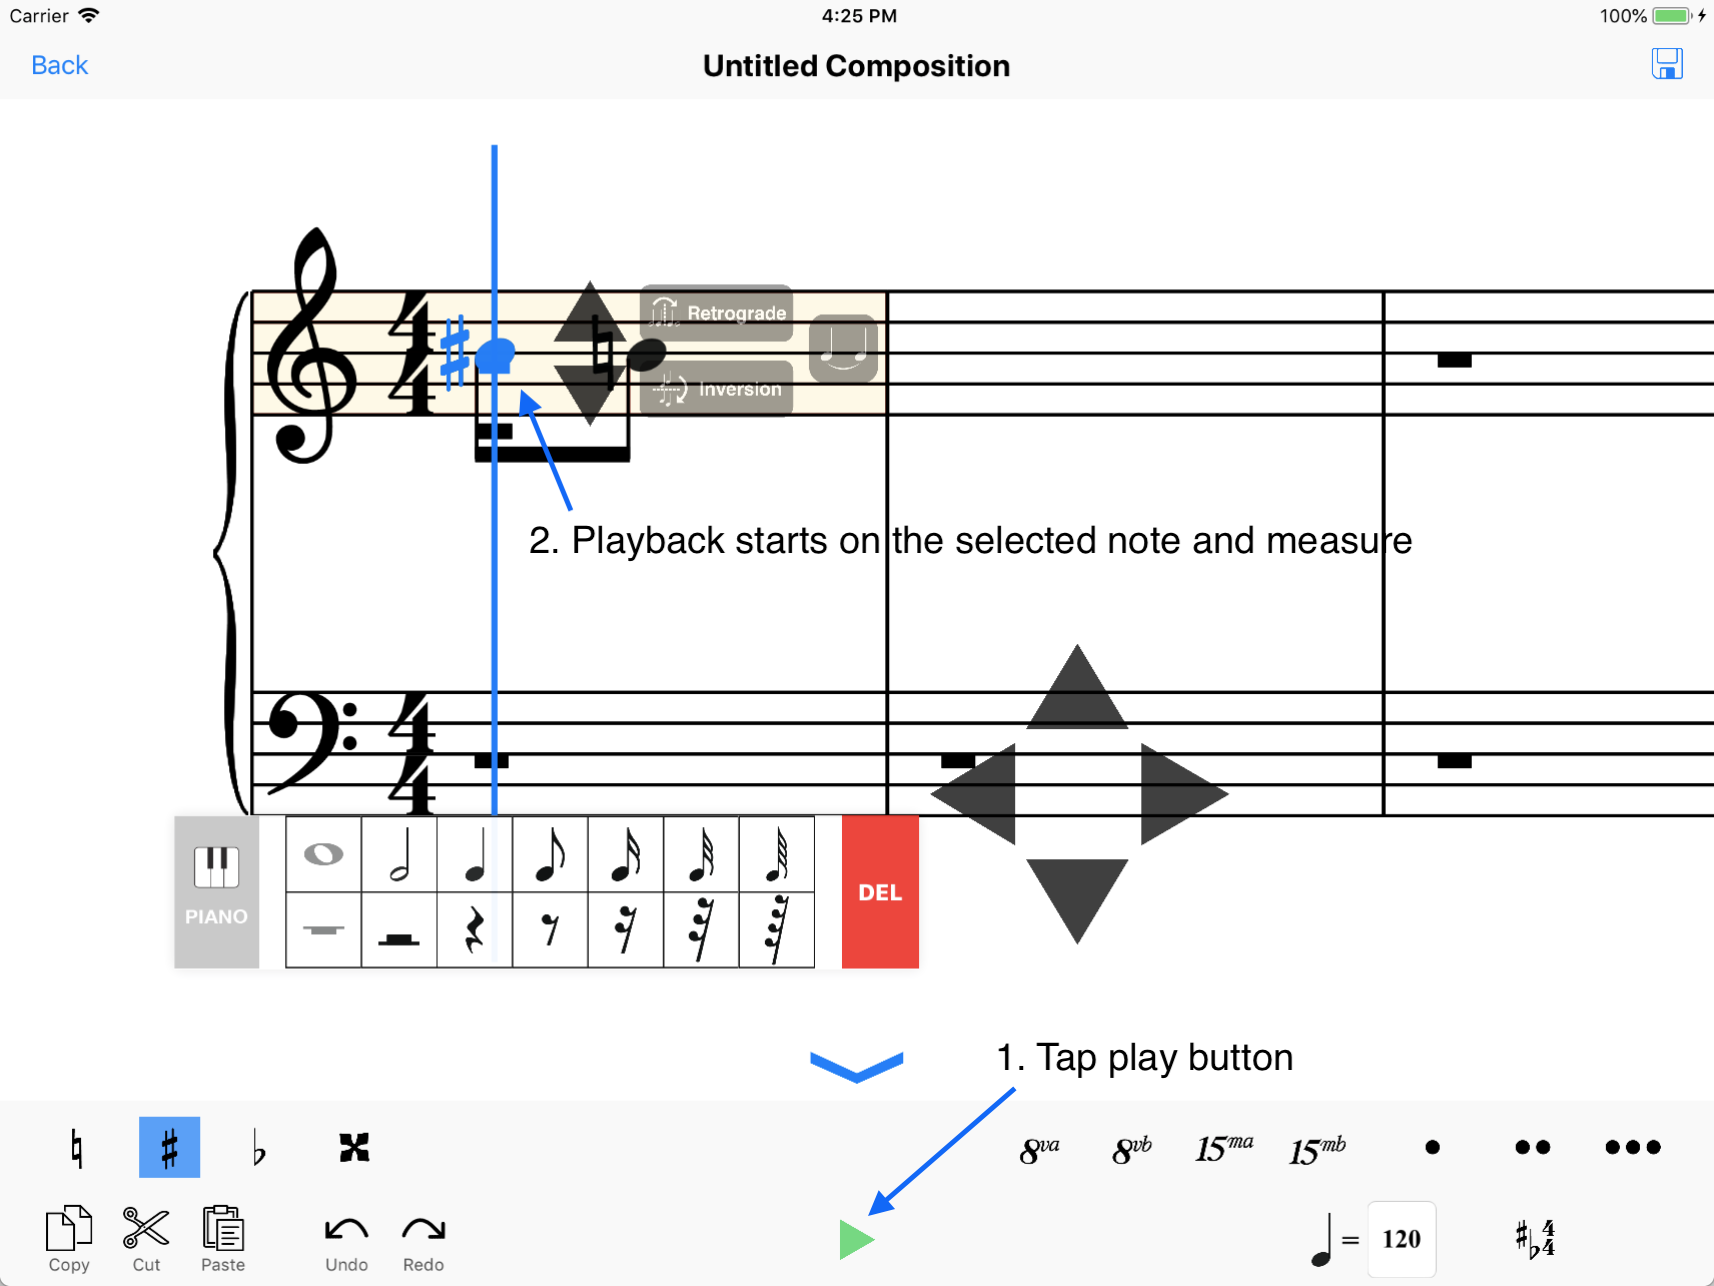
\includegraphics[scale=0.5]{Play}
    \caption{Playing the composition.}
    \label{fig:play}
\end{figure}

\subsubsection{Saving the Composition}
To save the composition, the user must simply tap on the save button in the upper right corner of the toolbar (Figure \ref{fig:save}).

\begin{figure}[H]
	\centering
	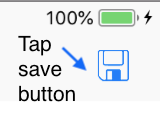
\includegraphics[scale=2]{Save}
    \caption{Saving the composition.}
    \label{fig:save}
\end{figure}

\subsubsection{Hiding and Showing the Bottom Menu}
To hide the bottom menu, the user must simply tap the arrow facing down on top of the bottom menu (Figure \ref{fig:hide}). To show it back again, the user must tap the arrow key facing up (Figure \ref{fig:show}).

\begin{figure}[H]
	\centering
	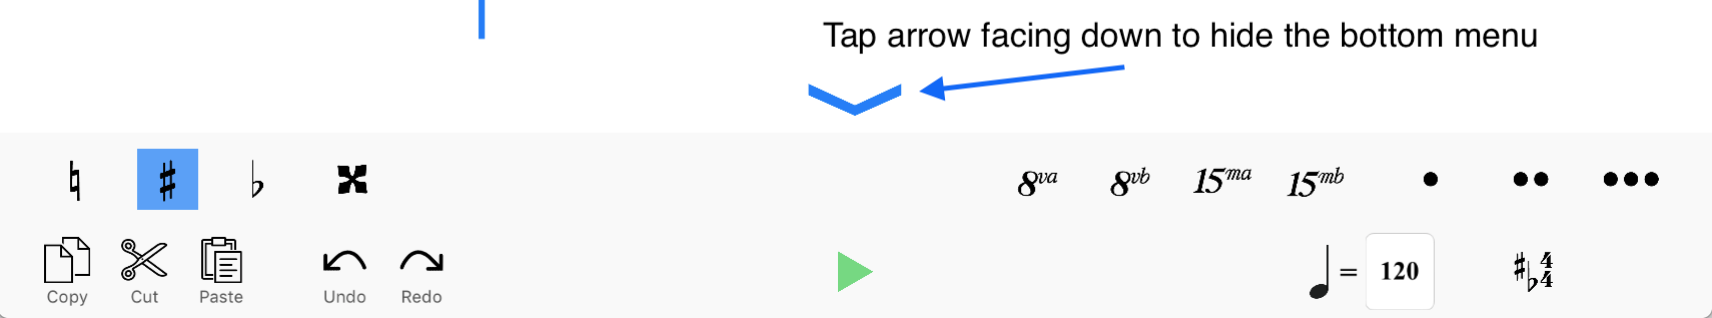
\includegraphics[scale=0.5]{Hide}
    \caption{Hiding the bottom menu.}
    \label{fig:hide}
\end{figure}

\begin{figure}[H]
	\centering
	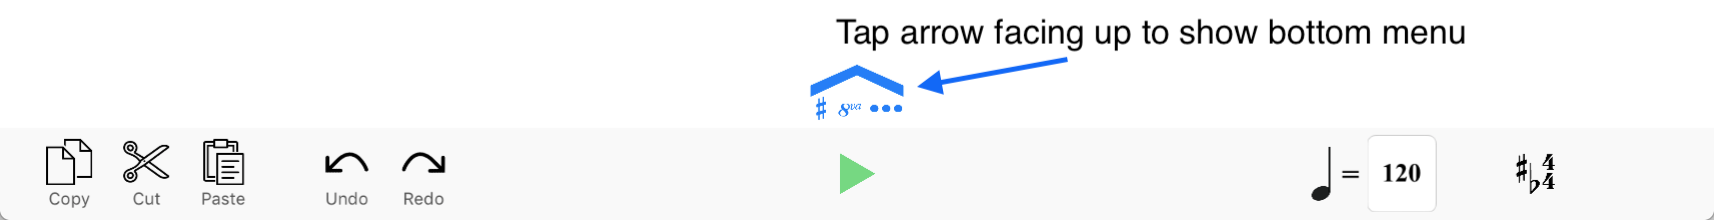
\includegraphics[scale=0.5]{Show}
    \caption{Showing the bottom menu.}
    \label{fig:show}
\end{figure}

\section{Experiment Design}

This chapter will describe the user stories and use cases that will be highlighted in the testing of the application. The intended users for the application will be expert composers who have at least 7 years of experience with composing music and amateur composers who have less than 7 years of experience composing music. These users should also have a basic knowledge of musical terms and are able to read and write musical notation. The details on the testing to be conducted on these users will also be discussed in this chapter.

\subsection{User Stories}
The user stories of the system will be focused on the main functions of the application and will highlight each specific need that the user has for the system. These user stories came from the users, representing the tasks that they need to perform on musical composition applications. These are created with the context that the system will run on a mobile platform with the mode of interaction mainly being touch gestures. 

\begin{enumerate}
\item As a user, I want to be able to create a blank composition, so that I can start my work
\item As a user, I want to be able to name my composition, so that I can differentiate it from my other compositions
\item As a user, I want to be able to save my composition, so that I can come back to it later
\item As a user, I want to be able to view all my saved compositions in a list, so that I can keep track of everything
\item As a user, I want to be able to open a saved composition so that I can perform more actions on it
\item As a user, I want to be able export my composition in a format that I can open in the composition application I use on my laptop
\item As a user, I want to be able to delete a composition, so I can discard compositions I do not work on anymore
\item As a user, I want to be able to add a chord progression in my composition, so that I do not need to individually add notes that belong to a progression
\item As a user, I want to be able to place a note in my composition, so that I can create my composition
\item As a user, I want to be able to select a single note, so that I can perform actions on it
\item As a user, I want to be able to change the pitch class of a note in my composition, so that I can make adjustments to my composition
\item As a user, I want to be able to change the type of a note in my composition, so that I can make the sound longer or shorter
\item As a user, I want to be able to erase a note in my composition, so that I can make space for other notes in my composition
\item As a user, I want to be able to highlight a group of notes in my composition, so that I can perform actions on the group
\item As a user, I want to be able to erase a highlighted group of notes in my composition, so that I can make space faster for other notes I'd like to place in my composition
\item As a user, I want to be able to place a rest in my composition, so I can have pauses in my composition
\item As a user, I want to be able to select a rest, so that I can perform actions on that rest
\item As a user, I want to be able to change the type of rest, so that I can change the length of pauses
\item As a user, I want to be able to highlight a group of rests, so that I can perform actions on the group of rests
\item As a user, I want to be able to erase a rest in my composition, so that I can make space for other rests or notes
\item As a user, I want to be able to change a rest in my composition, so that I can make adjustments to my composition
%\item As a user, I want to be able to move the position of a note in my composition, so that I can move that note to a better position
%\item As a user, I want to be able to move the position of a highlighted group of notes in my composition, so that I can reposition multiple notes at a time to a better position
\item As a user, I want to be able to hear the sound of the note I just added, so that I know I've added the correct sounding note
\item As a user, I want to be able to listen to a highlighted section of my composition, so that I can hear just a segment of my piece
\item As a user, I want to be able to listen to my whole composition, so that I can hear it as a whole
\item As a user, I want to be able to perform a swipe gesture that will generate a succession of notes based on the orientation of my gesture and my current composition because I'm interested in knowing what series of notes match my current composition
\item As a user, I want to be able to manipulate the generated series of notes, because the generated series of notes just needs a little bit more adjustments before I accept it into my composition
\item As a user, I want to be able to discard the series of notes generated by the application after a swipe gesture, so I do not have to delete them one by one
\item As a user, I want to be able to confirm the addition of the series of notes given by the application after a swipe gesture, so I can create my composition quickly
\item As a user I want to be able to undo an action or a series of actions, so that I can undo an unintended action or series of unintended actions quicker
\item As a user I want to be able to redo an action or a series of actions, so that I can redo an intended action or a series of intended actions quicker
\item As a user, I want to be able to reposition the menu because I want to place it where it is not an obstacle for me while composing
\item As a user, I want to be able to set the time signature of my composition
\item As a user, I want to be able to see the details of a single note, so that I can know the specifications of the note
\item As a user, I want to be able to see the details of a selected group of notes, so that I can know the specification of the selected group of notes
\item As a user, I want to be able to see the details of the generated series of notes like the pitch and type so that I can know what notes the system has generated after a gesture
\item As a user, I want to be able to set the clef of my composition
\item As a user, I want to be able to set the key signature of my composition
\item As a user, I want to be able to set the time signature of my composition
\item As a user, I want to be able to copy a highlighted group of notes and/or rests, so that I can copy a recurring segment in my composition
\item As a user, I want to be able to cut a highlighted group of notes and/or rests, so that I can copy a segment of my composition while at the same time making space for more notes
\item As a user, I want to be able to paste the copied or cut group of notes and/or rests onto my composition, so that I do not need to add a recurring segment in my composition manually all the time
%\item As a user, I want to be able to move the position of a rest, so that I can move that rest to a better position
%\item As a user, I want to be able to move the position of a selected group of rests, so that I can move multiple rests at a time to a better position
\item As a user, I want to be able to add accidentals to my notes, so that I can control the pitch of my notes
\item As a user, I want to be able to transpose a highlighted group of notes, so that I do not need to individually change the pitch of each note
\item As a user, I want to be able to perform retrograde inversion on a single note, so that I do not have to move it manually to invert it
\item As a user, I want to be able to perform retrograde inversion on a group of notes, so that I do not need to invert each note individually

\end{enumerate}

\subsection{Use Cases}

This section defines the several actions the users can perform within the system. These use cases were derived from the needs of the composers and the functions of Flow. The design of each use case will be based on fully dressed use cases with precision level 2 found in the book of \cite{alistair2001writing}. The headers in each use case will be: trigger, primary actor, supporting actors, preconditions, minimal guarantees, success guarantees, and process steps.

\textbf{Trigger} \\
The main situation or goal that the use case will be revolving around. 

\textbf{Primary Actor} \\
The main entity that will be performing or influencing situation or goal directly.

\textbf{Supporting Actors} \\
Additional entities that will be indirectly or directly influenced by the outcome of the situation. These entities can also be influencing the decision making or performance of the primary actor.

\textbf{Preconditions} \\
These conditions need to be followed before the process steps can be performed.

\textbf{Process Steps} \\
Each step will be performed by the primary actor to accomplish the goal.

\textbf{Minimal Guarantees} \\
Outcome or result that will occur in case a goal is not fully accomplished.

\textbf{Success Guarantees} \\
Outcome or result that occurs when a goal is fully accomplished.

%Trigger
%Primary Actor
%Supporting Actors
%Precondition
%Process Steps
%Minimal Guarantees
%Success Guarantees


%%Layout needs to be fixed

%Sprint 1
\subsubsection{Use Case 1: Add a Single Note}

\LTXtable{\textwidth}{longtables/use_case_1_lt}

%Sprint 1
\subsubsection{Use Case 2: Change a Single Note}

\LTXtable{\textwidth}{longtables/use_case_2_lt}

%Sprint 1
\subsubsection{Use Case 3: Delete a Single Note through the Side Menu}

\LTXtable{\textwidth}{longtables/use_case_3_lt}

\subsubsection{Use Case 4: Delete a Single Note through a Flick Gesture}

\begin{tabularx}{\textwidth}{|X|X|}
\hline
Trigger & 
The composer needs to delete a note quickly \\
\hline
Primary Actor & 
Composer\\
\hline
Supporting Actors & 
\begin{itemize}
\item Listener
\item Instrumentalist
\item Producer
\item Flow
\end{itemize} \\
\hline
Precondition & 
\begin{itemize}
\item The user has a composition open in Flow 
\item The deletion of the selected note is valid based on the set musical rules
\end{itemize} \\
\hline
Process Steps & 
\begin{enumerate}
\item The user performs a flick gesture on the note to be deleted
\item Flow removes the selected note from the composition
\end{enumerate} \\
\hline
Minimal Guarantees & 
\begin{itemize}
  \item A note will be deleted
  \item The side menu will return to being transparent
\end{itemize} \\
\hline
Success Guarantees & 
\begin{itemize}
  \item The selected note will be deleted
  \item The space occupied by the selected note will be freed
\end{itemize} \\
\hline
\end{tabularx}

\subsubsection{Use Case 5: Toggle Accidental Marks on Note Addition}

\LTXtable{\textwidth}{longtables/use_case_5_lt}

\subsubsection{Use Case 6: Transform a Note to its Dotted Version}

\LTXtable{\textwidth}{longtables/use_case_6_lt}

\subsubsection{Use Case 7: Horizontal Swipe Gesture to Generate a Series of Notes}

\LTXtable{\textwidth}{longtables/use_case_7_lt}

\subsubsection{Use Case 8: Delete a Highlighted Group of Notes or Rests}

\LTXtable{\textwidth}{longtables/use_case_8_lt}

\subsubsection{Use Case 9: Replace a Highlighted Group of Notes or Rests with a Single Note}

\LTXtable{\textwidth}{longtables/use_case_9_lt}

\subsubsection{Use Case 10: Replace a Highlighted Group of Notes or Rests with a Single Rest}

\LTXtable{\textwidth}{longtables/use_case_10_lt}


\subsubsection{Use Case 11: Single Note Transposition}

\begin{tabularx}{\textwidth}{|X|X|}
\hline
Trigger & 
The user needs to transpose a note to set its pitch higher \\
\hline
Primary Actor & 
Composer \\
\hline
Supporting Actors & 
\begin{itemize}
\item Listener
\item Instrumentalist
\item Producer
\item Flow
\end{itemize} \\
\hline
Precondition & 
\begin{itemize}
\item The user has a composition open in Flow
\item The transposition is valid based on the set musical rules
\end{itemize} \\
\hline
Process Steps & 
\begin{enumerate}
\item The user performs a two finger swipe gesture upwards on the desired note
\item Flow increases the pitch of the note
\end{enumerate} \\
\hline
Minimal Guarantees & 
\begin{itemize}
  \item None
\end{itemize} \\
\hline
Success Guarantees & 
\begin{itemize}
  \item The desired note will be transposed upwards
\end{itemize} \\
\hline
\end{tabularx}

\subsubsection{Use Case 12: Multiple Note Transposition}

\begin{tabularx}{\textwidth}{|X|X|}
\hline
Trigger & 
The user needs to transpose a group of note to set their pitch higher \\
\hline
Primary Actor & 
Composer \\
\hline
Supporting Actors & 
\begin{itemize}
\item Listener
\item Instrumentalist
\item Producer
\item Flow
\end{itemize} \\
\hline
Precondition & 
\begin{itemize}
\item The user has a composition open in Flow
\item The batch transposition is valid based on the set musical rules
\end{itemize} \\
\hline
Process Steps & 
\begin{enumerate}
\item The user highlights a group of notes
\item The user performs a two finger swipe gesture upwards on the highlighted group of notes
\item Flow increases the pitch of the highlighted group of notes
\end{enumerate} \\
\hline
Minimal Guarantees & 
\begin{itemize}
  \item None
\end{itemize} \\
\hline
Success Guarantees & 
\begin{itemize}
  \item The highlighted group of notes will be transposed upwards
\end{itemize} \\
\hline
\end{tabularx}


\subsubsection{Use Case 13: Retrograde a Collection of Notes}

\begin{tabularx}{\textwidth}{|X|X|}
\hline
Trigger & 
The user needs to retrograde a collection of notes \\
\hline
Primary Actor & 
Composer \\
\hline
Supporting Actors & 
\begin{itemize}
\item Listener
\item Instrumentalist
\item Producer
\item Flow
\end{itemize} \\
\hline
Precondition & 
\begin{itemize}
\item The user has a composition open in Flow
\item The retrograde does not violate the set musical rules
\end{itemize} \\
\hline
Process Steps & 
\begin{enumerate}
\item The user highlights a group of notes
\item The user performs a two finger flick gesture horizontally on top of the collection of notes
\item Flow retrogrades the collection of notes
\end{enumerate} \\
\hline
Minimal Guarantees & 
\begin{itemize}
  \item None
\end{itemize} \\
\hline
Success Guarantees & 
\begin{itemize}
  \item The collection of notes will be retrograded
\end{itemize} \\
\hline
\end{tabularx}

\subsubsection{Use Case 14: Invert a Collection of Notes}

\begin{tabularx}{\textwidth}{|X|X|}
\hline
Trigger & 
The user needs to invert a collection of notes \\
\hline
Primary Actor & 
Composer \\
\hline
Supporting Actors & 
\begin{itemize}
\item Listener
\item Instrumentalist
\item Producer
\item Flow
\end{itemize} \\
\hline
Precondition & 
\begin{itemize}
\item The user has a composition open in Flow
\item The inversion does not violate the set musical rules
\end{itemize} \\
\hline
Process Steps & 
\begin{enumerate}
\item The user highlights a group of notes
\item The user performs a two finger flick gesture vertically on top of the collection of notes
\item Flow inverts the collection of notes
\end{enumerate} \\
\hline
Minimal Guarantees & 
\begin{itemize}
  \item None
\end{itemize} \\
\hline
Success Guarantees & 
\begin{itemize}
  \item The collection of notes will be inverted
\end{itemize} \\
\hline
\end{tabularx}

\subsubsection{Use Case 15: Add a Chord}

\LTXtable{\textwidth}{longtables/use_case_15_lt}

\subsubsection{Use Case 16: Add a Single Rest}

\LTXtable{\textwidth}{longtables/use_case_16_lt}

\subsubsection{Use Case 17: Change a Single Rest}

\LTXtable{\textwidth}{longtables/use_case_17_lt}

%Sprint 1
\subsubsection{Use Case 18: Delete a Single Rest through the Side Menu}

\LTXtable{\textwidth}{longtables/use_case_18_lt}


\subsubsection{Use Case 19: Delete a Single Rest through Flick Gesture}

\begin{tabularx}{\textwidth}{|X|X|}
\hline
Trigger & 
The composer needs to delete a rest quickly \\
\hline
Primary Actor & 
Composer\\
\hline
Supporting Actors & 
\begin{itemize}
\item Listener
\item Instrumentalist
\item Producer
\item Flow
\end{itemize} \\
\hline
Precondition & 
\begin{itemize}
\item The user has a composition open in Flow 
\item The deletion of the selected rest is valid based on the set musical rules
\end{itemize} \\
\hline
Process Steps & 
\begin{enumerate}
\item The user performs a flick gesture on the rest to be deleted
\item Flow removes the selected rest from the composition
\end{enumerate} \\
\hline
Minimal Guarantees & 
\begin{itemize}
  \item A rest will be deleted
  \item The side menu will return to being transparent
\end{itemize} \\
\hline
Success Guarantees & 
\begin{itemize}
  \item The selected rest will be deleted
  \item The space occupied by the selected rest will be freed
\end{itemize} \\
\hline
\end{tabularx}

\subsubsection{Use Case 20: Listen to a Single Note}

\begin{tabularx}{\textwidth}{|X|X|}
\hline
Trigger & 
The user needs to listen to a single note \\
\hline
Primary Actor & 
Composer \\
\hline
Supporting Actors & 
\begin{itemize}
\item Listener
\item Instrumentalist
\item Producer
\item Flow
\end{itemize} \\
\hline
Precondition & 
\begin{itemize}
\item The user has a composition open in Flow
\end{itemize} \\
\hline
Process Steps & 
\begin{enumerate}
\item The user selects a note
\item The user taps on the play button
\item Flow will play the sound of the selected note
\end{enumerate} \\
\hline
Minimal Guarantees & 
\begin{itemize}
 \item The icon for the play button will become a pause symbol then return to a play symbol once the composition is done playing
\end{itemize} \\
\hline
Success Guarantees & 
\begin{itemize}
  \item The selected note will be played
\end{itemize} \\
\hline
\end{tabularx}

\subsubsection{Use Case 21: Listen to a Highlighted Section of the Composition}

\LTXtable{\textwidth}{longtables/use_case_21_lt}

\subsubsection{Use Case 22: Listen to the Whole Composition}

\begin{tabularx}{\textwidth}{|X|X|}
\hline
Trigger & 
The user needs to listen to the whole composition \\
\hline
Primary Actor & 
Composer \\
\hline
Supporting Actors & 
\begin{itemize}
\item Listener
\item Instrumentalist
\item Producer
\item Flow
\end{itemize} \\
\hline
Precondition & 
\begin{itemize}
\item The user has a composition open in Flow
\item The composition is not empty
\item The user has no notes selected or highlighted
\end{itemize} \\
\hline
Process Steps & 
\begin{enumerate}
\item The user taps on the play button
\item Flow will play the whole composition
\end{enumerate} \\
\hline
Minimal Guarantees & 
\begin{itemize}
  \item The icon for the play button will become a pause symbol then return to a play symbol once the composition is done playing
\end{itemize} \\
\hline
Success Guarantees & 
\begin{itemize}
  \item The whole composition will be played correctly until the last note or rest
\end{itemize} \\
\hline
\end{tabularx}

\subsubsection{Use Case 23: View the Details of a Single Note or Rest}

\begin{tabularx}{\textwidth}{|X|X|}
\hline
Trigger & 
The user needs to know the details of a single note or rest\\
\hline
Primary Actor & 
Composer \\
\hline
Supporting Actors & 
\begin{itemize}
\item Listener
\item Instrumentalist
\item Producer
\item Flow
\end{itemize} \\
\hline
Precondition & 
\begin{itemize}
\item The user has a composition open in Flow
\item The note or rest is in the composition
\end{itemize} \\
\hline
Process Steps & 
\begin{enumerate}
\item The user selects a note or rest
\item The user taps on the toggle details option
\item Flow will display the details of the note or rest
\end{enumerate} \\
\hline
Minimal Guarantees & 
\begin{itemize}
  \item The toggle button graphic will change
\end{itemize} \\
\hline
Success Guarantees & 
\begin{itemize}
  \item The toggle button graphic will change
  \item The details of the selected note or rest will be displayed 
\end{itemize} \\
\hline
\end{tabularx}


\subsubsection{Use Case 24: View the Details of a Highlighted Group of Notes or Rests}

\LTXtable{\textwidth}{longtables/use_case_24_lt}

\subsubsection{Use Case 25: Copy and Paste a Single Note or Rest}

\LTXtable{\textwidth}{longtables/use_case_25_lt}

\subsubsection{Use Case 26: Cut and Paste a Single Note or Rest}

\LTXtable{\textwidth}{longtables/use_case_26_lt}

\subsubsection{Use Case 27: Copy and Paste a Group of Notes or Rests}

\LTXtable{\textwidth}{longtables/use_case_27_lt}

\subsubsection{Use Case 28: Cut and Paste a Group of Notes or Rests}

\LTXtable{\textwidth}{longtables/use_case_28_lt}

%Sprint 1
\subsubsection{Use Case 29: Create Blank Composition}

\LTXtable{\textwidth}{longtables/use_case_29_lt}

%Sprint 1
\subsubsection{Use Case 30: View Existing Composition}

\begin{tabularx}{\textwidth}{|X|X|}
\hline
Trigger & 
The user needs to view an existing composition \\
\hline
Primary Actor & 
Composer \\
\hline
Supporting Actors & 
\begin{itemize}
\item Listener
\item Instrumentalist
\item Producer
\item Flow
\end{itemize} \\
\hline
Precondition & 
\begin{itemize}
\item The user is in the main menu screen
\item The composition is in storage
\item The composition is not corrupted
\end{itemize} \\
\hline
Process Steps & 
\begin{enumerate}
\item The user taps on the composition from the main menu
\item Flow opens the selected composition
\end{enumerate} \\
\hline
Minimal Guarantees & 
\begin{itemize}
  \item None
\end{itemize} \\
\hline
Success Guarantees & 
\begin{itemize}
  \item The selected composition will open
\end{itemize} \\
\hline
\end{tabularx}

%Sprint 1
\subsubsection{Use Case 31: Delete Existing Composition}

\begin{tabularx}{\textwidth}{|X|X|}
\hline
Trigger & 
The user needs to delete a composition \\
\hline
Primary Actor & 
Composer \\
\hline
Supporting Actors & 
\begin{itemize}
\item Listener
\item Instrumentalist
\item Producer
\item Flow
\end{itemize} \\
\hline
Precondition & 
\begin{itemize}
\item The user is in the main menu screen
\item The composition is in storage
\end{itemize} \\
\hline
Process Steps & 
\begin{enumerate}
\item The user taps on the delete composition button from the main menu
\item The user taps confirm
\item Flow deletes the selected composition
\end{enumerate} \\
\hline
Minimal Guarantees & 
\begin{itemize}
  \item None
\end{itemize} \\
\hline
Success Guarantees & 
\begin{itemize}
  \item The selected composition will be deleted
  \item Memory taken by the deleted composition will be freed
\end{itemize} \\
\hline
\end{tabularx}

\subsubsection{Use Case 32: Redo an Action}

\begin{tabularx}{\textwidth}{|X|X|}
\hline
Trigger & 
The user wants to redo an action\\
\hline
Primary Actor & 
Composer \\
\hline
Supporting Actors & 
\begin{itemize}
\item Listener
\item Instrumentalist
\item Producer
\item Flow
\end{itemize} \\
\hline
Precondition & 
\begin{itemize}
\item An undo action has been performed at least once
\item Redo action is valid based on the state of the composition
\item Redo action is valid based on the set musical rules
\end{itemize} \\
\hline
Process Steps & 
\begin{enumerate}
\item The user taps on the redo button
\item Flow performs the undone action
\end{enumerate} \\
\hline
Minimal Guarantees & 
\begin{itemize}
  \item The redo button will give feedback 
\end{itemize}\\
\hline
Success Guarantees & 
\begin{itemize}
  \item The correct action is redone
\end{itemize} \\
\hline
\end{tabularx}

\subsubsection{Use Case 33: Undo an Action}

\begin{tabularx}{\textwidth}{|X|X|}
\hline
Trigger & 
The user wants to undo an action \\
\hline
Primary Actor & 
Composer \\
\hline
Supporting Actors & 
\begin{itemize}
\item Listener
\item Instrumentalist
\item Producer
\item Flow
\end{itemize} \\
\hline
Precondition & 
\begin{itemize}
\item At least one action has been performed
\item Undo action is valid based on the state of the composition
\item Undo action is valid based on the set musical rules
\end{itemize} \\
\hline
Process Steps & 
\begin{enumerate}
\item The user taps on the undo button
\item Flow undos the last action
\end{enumerate} \\
\hline
Minimal Guarantees & 
\begin{itemize}
  \item The undo button will give feedback
\end{itemize} \\
\hline
Success Guarantees & 
\begin{itemize}
  \item The correct action is undone
\end{itemize} \\
\hline
\end{tabularx}

\subsubsection{Use Case 34: Select a Single Note or Rest}

\begin{tabularx}{\textwidth}{|X|X|}
\hline
Trigger & 
The user needs to select a note or rest \\
\hline
Primary Actor & 
Composer \\
\hline
Supporting Actors & 
\begin{itemize}
\item Listener
\item Instrumentalist
\item Producer
\item Flow
\end{itemize} \\
\hline
Precondition & 
\begin{itemize}
\item The user has a composition open in Flow
\end{itemize} \\
\hline
Process Steps & 
\begin{enumerate}
\item The user taps on a single note or rest
\item Flow displays that the single note or rest is selected
\end{enumerate} \\
\hline
Minimal Guarantees & 
\begin{itemize}
  \item None
\end{itemize} \\
\hline
Success Guarantees & 
\begin{itemize}
  \item The look of a selected note or rest is differentiated from the unselected notes and rests
  \item The correct note or rest is selected
  \item Actions can be performed on the selected note or rest
\end{itemize} \\
\hline
\end{tabularx}


\subsubsection{Use Case 35: Highlight a Group of Notes or Rests}

\LTXtable{\textwidth}{longtables/use_case_35_lt}

\subsubsection{Use Case 36: Rename the Composition from the Composition Environment}

\LTXtable{\textwidth}{longtables/use_case_36_lt}

\subsubsection{Use Case 37: Rename the Composition from the Main Menu}

\LTXtable{\textwidth}{longtables/use_case_37_lt}

\subsubsection{Use Case 38: Move the Note Menu to a Different Position}

\begin{tabularx}{\textwidth}{|X|X|}
\hline
Trigger & 
The user needs to move the note menu to a different position\\
\hline
Primary Actor & 
Composer \\
\hline
Supporting Actors & 
\begin{itemize}
\item Listener
\item Instrumentalist
\item Producer
\item Flow
\end{itemize} \\
\hline
Precondition & 
\begin{itemize}
\item The user has a composition open in Flow
\item The new location for the note menu is valid
\end{itemize} \\
\hline
Process Steps & 
\begin{enumerate}
\item The user drags the note menu to the desired location
\item Flow will reposition the note menu during the drag gesture
\end{enumerate} \\
\hline
Minimal Guarantees & 
\begin{itemize}
  \item None
\end{itemize} \\
\hline
Success Guarantees & 
\begin{itemize}
  \item The note menu will move to its desired location
\end{itemize} \\
\hline
\end{tabularx}

\subsubsection{Use Case 39: Export to MusicXML from the Main Menu}

\LTXtable{\textwidth}{longtables/use_case_39_lt}

\subsubsection{Use Case 40: Toggle Notes to Rests to Chords in the Side Menu}

\LTXtable{\textwidth}{longtables/use_case_40_lt}

\subsubsection{Use Case 41: Change the Time Signature of the Composition}

\LTXtable{\textwidth}{longtables/use_case_41_lt}

\subsubsection{Use Case 42: Change the Key Signature of the Composition}

\LTXtable{\textwidth}{longtables/use_case_42_lt}

\subsubsection{Use Case 43: Change a Clef}

\LTXtable{\textwidth}{longtables/use_case_43_lt}

\subsection{User Test Plan}

The objective of the tests will be to determine if the interaction and design of the system augments the user experience of the composer while interacting with Flow. The functionality will also be closely monitored to see if there are glitches or bugs that require additional fixes in the development side. These bugs or glitches will warrant an intervention from the researchers during the testing.

The tests will be conducted in an environment where audio and visual disturbances are at a minimum. This is to ensure that the researchers are able to analyze clear audio and video data from the recording devices used during the testing. This is also to ensure that the tester is not disutbred during the testing. The setups used accross all the user tests are 4 kinds of Flow system prototpyes, 1 created using a prototyping tool called InVision, and 3 coded in Swift; 2 kinds of commercially available notation applications in the App Storem, Notion and Komp; and the traditional form of composition which is using music sheets and writing materials. Notation softwares and the Flow prototypes will be launched on a mobile platform, namely an IPad tablet.

Before starting the test, testers will be given a consent form. If they agree with the terms and continue with the testing, the tasks indicated in Section \ref{sec:tasks} will be done for each test setup (indicated in Section \ref{sec:test-setups}) that is appropriate. Before the start of the test where the tester start to accomplish tasks or use cases for the test setup, they will be given a brief description of the objectives of the study along with overview of the tasks or use cases. 

The researchers will be collecting quantitative and qualitative data. There will be tasks that the testers will be asked to accomplish, during iteration 1 and 2, after those tasks, data will be collected through an online form open after testing. During iteration 3 and 4, data will be collected during each use case through an online form. There will be video recording of the testers face and hand movements to be analyzed by the researchers during the testing. After the testing, for iteration 1 and 2, testers are then asked to answer a questionnaire to evaluate the quality of the application, and for iteration 3 and 4, testers are given a brief interview about their thoughts on each of the setups and the application.

During the first two (2) iterations, five (5) subjects of both genders aged 18-40 were recruited through snowball sampling method to take part in the data collection and testing. These subjects were categorized into two (2) user groups based on musical composition experience: amateur, and experienced. For the third iteration, fifteen (15) subjects of the same demographics took part in the testing. In the last iteration, ten (10) subjects took part. 

\subsection{Test Setups}
\label{sec:test-setups}

The setups between the preliminary testing and the subsequent testing were different. This was made so because the main goal of the preliminary testing was to gather feedback on the interaction design and help improve the system while it was still being developed. Other applications did not matter as much and were only used to gain insight on their interactions and how they could be used to improve the system. Although the goal of the subsequent tests were still to gather feedback and improve the system, they were also made to compare the system against similar musical composition applications. 

\subsubsection{Preliminary Testing Setups}

The test setups are meant to observe how existing methods of composition work and how their interactions could be used in Flow. The tasks enumerated in Section \ref{sec:preliminary-tasks} will be used in each test setup whenever possible since some tasks can only be accomplished within a specific setup. 

There will be 3 different test setups to be used during user testing namely:

\begin{enumerate}
\item Tester composing using music sheets
\item Tester composing using Komp
\item Tester composing using Flow
\end{enumerate}

For the first iteration, there will be 4 tasks for each of these setups with 1 special task for the setup using Flow:

\begin{enumerate}
\item Add a Note
\item Add a Series of Notes
\item Change a Note
\item Special Task - Delete a Series of Notes
\item Compose for 3 Minutes
\end{enumerate}

For the second iteration, there will be 7 tasks for each of these setups and 3 additional special tasks for the setup using Flow:

\begin{enumerate}
\item Add notes to fill 2 measures
\item Change Time Signature to 3/4
\item Special Task - Empty one measure
\item Special Task - Empty composition
\item Add enough notes to fill 2 measures in 2 staffs
\item Add an accidental to 2 notes
\item Remove placed accidentals 
\item Change Key Signature
\item Special Task - Replace a group of notes with a single note
\item Create or recreate a composition (Exactly 4 measures)
\subitem Twinkle Twinkle Little Star
\subitem Canon in D
\subitem Ode to Joy 
\end{enumerate}



The first setup simulates the traditional way of musical composition. This is through music sheets and a writing instrument. Traditional music sheets will be provided by the researchers as well as a choice of using a pen or pencil for writing musical elements. The composers are free to use as much music sheets as they want for drafting and experimenting with their composition as long as the time and resources provided by the researchers allow them.

The second setup will be through an existing mobile application for iOS platforms, komp. Since the method of input in komp is similar to writing in music sheets, this setup will mainly be done to see how the interaction for traditional musical composition will work when applied to mobile devices. The researchers expect this setup to have similar results with the first setup and any data collected in this setup will be used to evaluate Flow.

The third setup will be focused on the composer using the developed system, Flow. During the early periods of testing, a mid-fidelity InVision prototype will be used as a substitute. Using this prototype, the only task that the composer will be able to do is to explore the application. The main goal of this is to develop and improve the interaction design of the application. One a high-fidelity prototype has been developed, all tasks will be performed in the testing.

\subsubsection{Subsequent Testing Setups}

In the subsequent tests, Flow was compared against other musical notation applications. For each setup, the users had to go through the use cases listed in \ref{sec:use-cases} and perform the tasks outlined in \ref{sec:subsequent-tasks}. Note that these setups were given in random order and that the application developed by the researchers was not disclosed to prevent bias.

\begin{enumerate}
\item Tester composing using Notion
\item Tester composing using komp
\item Tester composing using Flow
\end{enumerate}

The first setup makes use of what is said to be the most popular musical notation application for mobile. For the second setup, komp is retained from the preliminary testing so that users can experience a traditional method of notation while on the iPad. The last setup makes use of the system developed by the researchers.

\subsubsection{Use Cases}
\label{sec:use-cases}

For the subsequent test setups, the testers had to go perform use cases. These use cases were an attempt to simulate different musical composition scenarios. 

\begin{enumerate}
    \item Compose a familiar song (Twinkle Twinkle Little Star/Happy Birthday)
    \item Compose from scratch
    \item Modify a composition (Ode to Joy/Amazing Grace)
\end{enumerate}


\subsection{Tasks}
\label{sec:tasks}

Similar to the test setups, the tasks differed greatly between the preliminary testing and subsequent testing. Tasks were generalized in the subsequent testing to make it easier for the testers to compare the different applications.

\subsubsection{Preliminary Testing Tasks}
\label{sec:preliminary-tasks}

Some tasks may be omitted in different test setups when a crucial function to carry out the task is unavailable. During the final task, testers are encouraged to speak aloud their concerns and opinions regarding the application.

% TODO update this list
\begin{enumerate}
\item Add a note in the composition
\item Add a series of notes
\item Change a note
\item Compose a musical piece within 10 minutes
%\item Compose a musical piece worth 2 staffs without using gestures
\item Free roam the application for 3-5 minutes
\end{enumerate}

\subsubsection{Subsequent Testing Tasks}
\label{sec:subsequent-tasks}

Since one of the goals of the subsequent tests was to compare how the interaction was against similar applications, the tasks were greatly simplified and generalized. Testers were also allowed to perform the tasks in any order they wanted and as much repititions it took for them to get acquainted with the specific task or action. These tasks were repeated for each of the use cases mentioned in \ref{sec:use-cases}.

\begin{enumerate}
  \item Select/highlight notes/chords
  \item Add notes/chords
  \item Edit notes/chords
  \item Delete notes/chords
  \item Cut, copy, or paste notes/chords
  \item Undo/redo an action
  \item Play the composition
\end{enumerate}

